\documentclass[journal]{IEEEtran}

\pdfminorversion=4

\usepackage[english]{babel}
\usepackage{xcolor}
\usepackage[table]{xcolor}
\usepackage{tabulary,booktabs,multirow}
\usepackage{listings}
\usepackage{hyperref}
\usepackage[font=small,labelfont=bf,skip=16pt]{caption}
\usepackage{subcaption}
\usepackage{tikz,float}
\usepackage[ruled,vlined]{algorithm2e}
\usepackage{orcidlink}
\usetikzlibrary{bayesnet,arrows}
\usetikzlibrary{shapes.geometric,positioning,arrows.meta,calc}
\tikzset{>=latex}
\usepackage{amsmath,amssymb,bm}
\usepackage{algorithm2e} 
\usepackage{cleveref}
\usepackage{cuted}
\usepackage{xcolor}
\usetikzlibrary{backgrounds}
\usepackage{stfloats} % allow bottom-placed figure* on the page where it is issued
\usepackage{cuted}    % full-width non-floating strip: page-1 teaser above the abstract
\setlength\stripsep{0pt plus 1pt minus 1pt} % tight gap between the title block and the teaser
\usepackage[printonlyused,withpage]{acronym}

% Math operators
\DeclareMathOperator{\E}{\mathbb{E}}
\DeclareMathOperator{\R}{\mathbb{R}}
\DeclareMathOperator{\N}{\mathbb{N}}
\DeclareMathOperator*{\argmax}{arg\,max}
\DeclareMathOperator*{\argmin}{arg\,min}
\DeclareMathAlphabet{\mathcal}{OMS}{cmsy}{m}{n}

% Theorem package
\usepackage{ntheorem}
\theoremseparator{:}

% \usepackage{orcidlink}
% \usepackage[english]{babel}
% \usepackage{soul}
% \usepackage{color}
% \usepackage{tabulary}
% \usepackage{booktabs}
% \usepackage{listings}
% \usepackage{multicol}
% \usepackage{enumitem}
% \usepackage{pifont}
% \usepackage[nointegrals]{wasysym}
% \usepackage{syntax}
% \usepackage{textcomp}
% % \usepackage{amsmath,accents}
% \usepackage[font=small,labelfont=bf,skip=16pt]{caption}
% \usepackage{hyperref}
% \usepackage[toc,acronym,nonumberlist,nomain]{glossaries}		% This has to load after hyperref package
% \usepackage{tikz,float,epsf, caption}
% \usepackage{amssymb}  % assumes amsmath package installed
% \usepackage{bm}
% \usepackage{multirow}
% \usepackage{booktabs}
% \usepackage[printonlyused,withpage]{acronym}
% \usepackage{pythonhighlight}
% \usepackage{cuted}
% \usepackage[position=bottom]{subfig}
% \usetikzlibrary{bayesnet}
% \usetikzlibrary{arrows}
% \tikzset{>=latex}
% \DeclareMathOperator{\E}{\mathbb{E}}
% \DeclareMathOperator{\R}{\mathbb{R}}
% \DeclareMathOperator{\N}{\mathbb{N}}
% \DeclareMathOperator*{\argmax}{arg\,max}
% \DeclareMathOperator*{\argmin}{arg\,min}
% \DeclareMathAlphabet{\mathcal}{OMS}{cmsy}{m}{n}
% \usepackage{ntheorem}
% \theoremseparator{:}
% % \newtheorem{hyp}{Hypothesis}

% \usepackage{graphicx}
% \usepackage{subcaption}
% \usepackage{caption} % For \captionof

% \usepackage{listings}


% \usepackage[ruled,vlined]{algorithm2e}  % for pseudocode
% \usepackage{amsmath, amssymb}           % math symbols
% \usepackage{graphicx}                   % figures if needed
% \usepackage{hyperref}                   % clickable refs
% \usepackage{cleveref}                   % smart references (e.g., \Cref)
% \usepackage{xcolor}                     % colors if you want to highlight

% ---------- Macros ----------
\newcommand{\Diffusion}{\pi_{\text{diff}}}   % shorthand for diffusion policy
\newcommand{\Dataset}{\mathcal{D}}           % shorthand for dataset
\newcommand{\Mask}{\mathcal{M}}              % shorthand for cloth mask

% \captionsetup[lstlisting]{name=Program}

\renewcommand{\lstlistingname}{Program}

\lstdefinestyle{pythonstyle}{
    language=Python,
    basicstyle=\ttfamily\small,
    breaklines=false,
    commentstyle=\color{green!50!black},
    keywordstyle=\color{blue},
    stringstyle=\color{red},
    numbers=left,
    numberstyle=\tiny\color{grey},
    numbersep=5pt,
    frame=single,
    framesep=15pt,
    rulecolor=\color{black!30},
    showstringspaces=false,
    tabsize=4
}
%
% Compiler warnings
%
\hfuzz=10pt 
\vfuzz=10pt
\hbadness=10000
\vbadness=10000

%
% Configure code listings
%
\lstset {
	language=Java,
	basicstyle=\footnotesize\ttfamily\singlespacing,
	showstringspaces=false,
	keywordstyle=\color[RGB]{0, 0, 240},
	stringstyle=\color[RGB]{240, 0, 0},
	commentstyle=\color[RGB]{0, 144, 0},
	numberstyle=\tiny,
	basewidth=0.54em,
	tabsize=2,
	captionpos=b,
	frame=tb,
	framesep=10pt,
	aboveskip=8pt,
	belowskip=0pt,
	abovecaptionskip = 16pt,
	breakindent=24pt,
	breaklines=true,
	numberbychapter=true
}

%
% Console output
%
\lstdefinestyle{console} {
	language=bash,
	basicstyle=\footnotesize\ttfamily\singlespacing,
	backgroundcolor=\color[RGB]{248, 247, 242},
	upquote=true,
	frame=single,
	framerule=0pt,
	breakindent=0pt,
	breaklines=true,
	aboveskip=0pt,
	belowskip=4pt,
	xleftmargin=10pt,
	xrightmargin=10pt
}


\title{LaGarNet: Latent World Models for Quasi-Static Pick-and-Place Garment Flattening}

% \author{Anonymous Authors}

\author{
Halid Abdulrahim Kadi$^{1}$,~\IEEEmembership{Member,~IEEE},~\orcidlink{0000-0001-9290-467X},
John Oyekan$^{1}$,~\IEEEmembership{Member,~IEEE},~\orcidlink{0000-0001-6578-9928}
, and
Kasim Terzi{\'c}$^{2}$,~\IEEEmembership{Member,~IEEE},~\orcidlink{0000-0001-6692-209X}

\thanks{$^{1}$~Department of Computer Science, University of York.}
\thanks{$^{2}$~School of Computer Science, University of St Andrews.}

\thanks{The initial phase of this work is supported by a Scholarship from the School of Computer Science at the University of St Andrews. The resubmission phase was supported by the Engineering and Physical Sciences Research Council (EPSRC) under the DIGI-CORTEX project.}}



\begin{document}

\maketitle

\begin{strip}
    \centering
    \captionsetup{type=figure}% strip is not a float; let \caption/\subfloat behave as if it were
    \vspace{-13mm}% IEEEtran adds a fixed skip after the title block; pull the teaser up
    
    % --- ROW 1 ---
    
    % First Subfigure: Simulation vs Real Goals
    \subfloat[Simulated garments' initial and goal states.\label{fig:sim-train-init}]{
        \begin{minipage}[c]{0.300\textwidth}
            \centering
            % Grouping the two original sub-images side-by-side
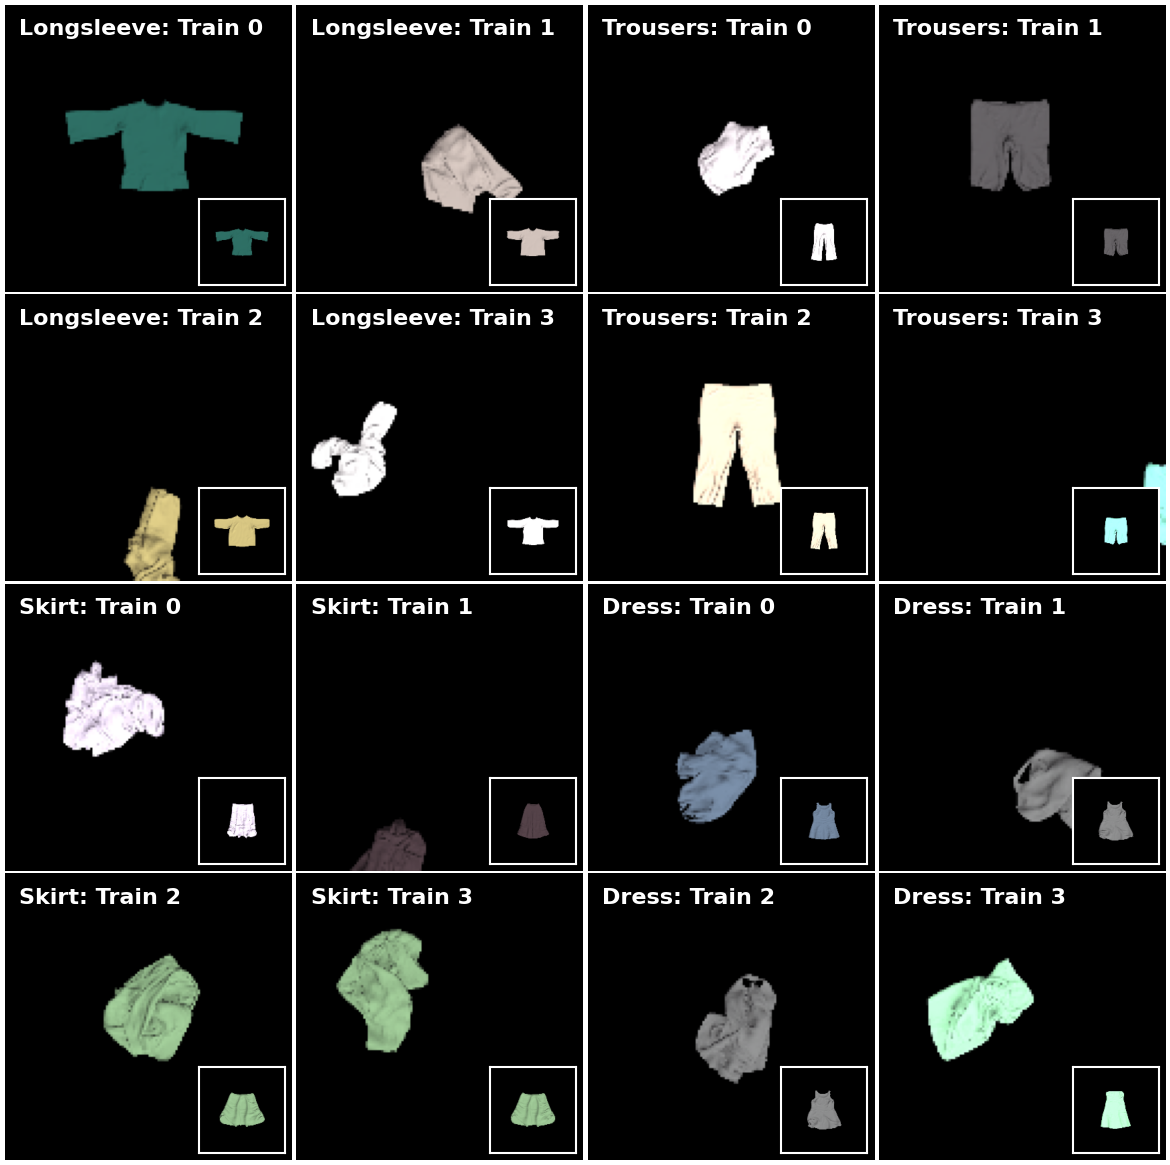
\includegraphics[width=1.0\linewidth]{plots/combined_garments_4x4_with_goals.png}\hfill
        \end{minipage}
    }
    % Second Subfigure: Real Garments
    \subfloat[Garments used for real-world evaluation. \label{fig:real-garments}]{
        \begin{minipage}[c]{0.415\textwidth}
            \centering
            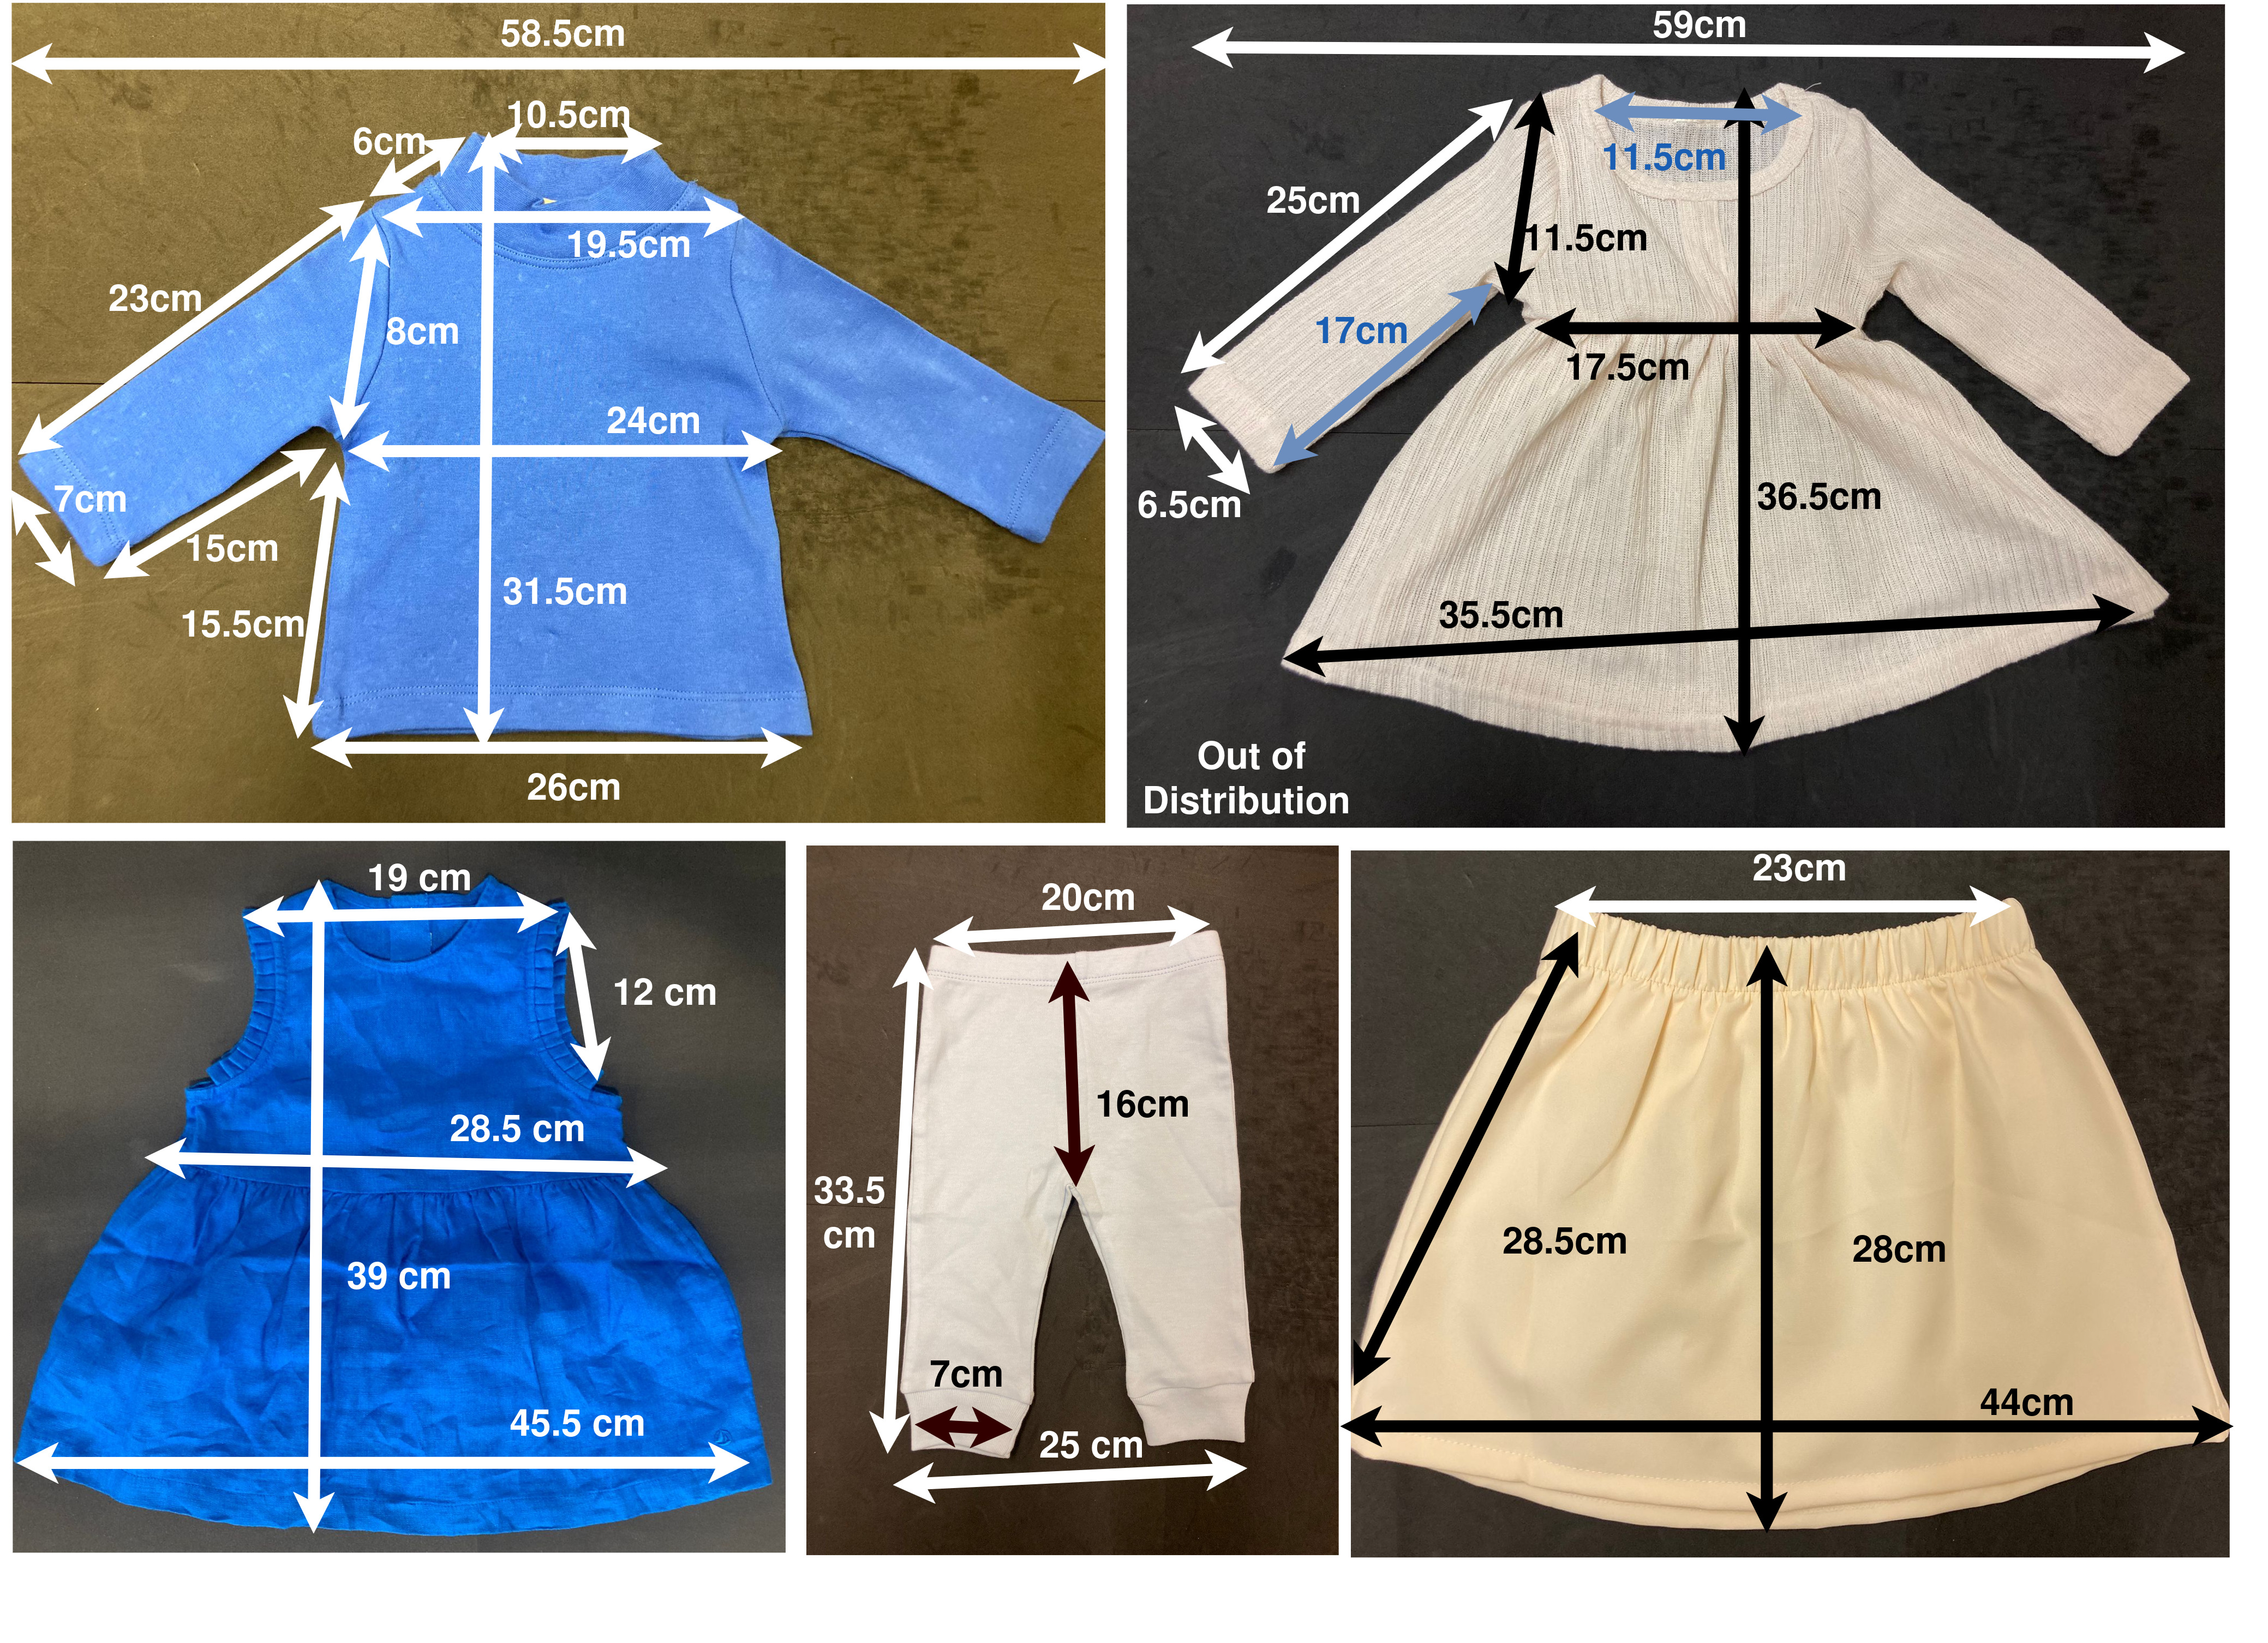
\includegraphics[width=1.0\linewidth]{plots/lagarnet-real-garments.jpg}
        \end{minipage}
    }
    % Second Subfigure: Real Garments
    \subfloat[UR5e flattening a skirt. \label{fig:ur5e-onrobot}]{
        \begin{minipage}[c]{0.222\textwidth}
            \centering
            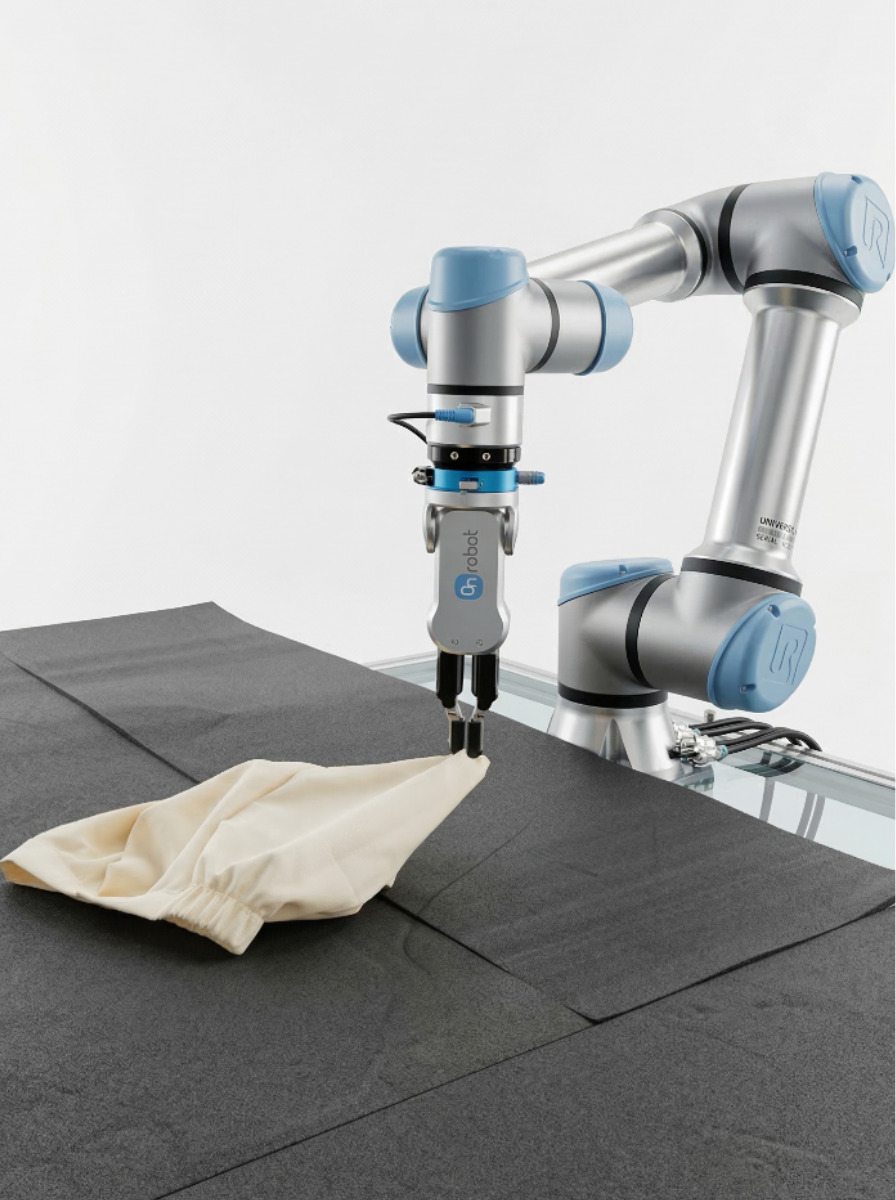
\includegraphics[width=1.0\linewidth]{plots/lagarnet-real-setup.jpg}
        \end{minipage}
    }
    
    \vspace{0.12cm} % Adds breathing room between the rows
    
    % --- ROW 2 ---
    
    % Third Subfigure: Spans the entire bottom row
    \subfloat[A qualitative demonstration of LaGarNet flattening a real dress.  \label{fig:ur3e-real-action-inference}]{
        \begin{minipage} [c]{0.985\textwidth}
            \centering
            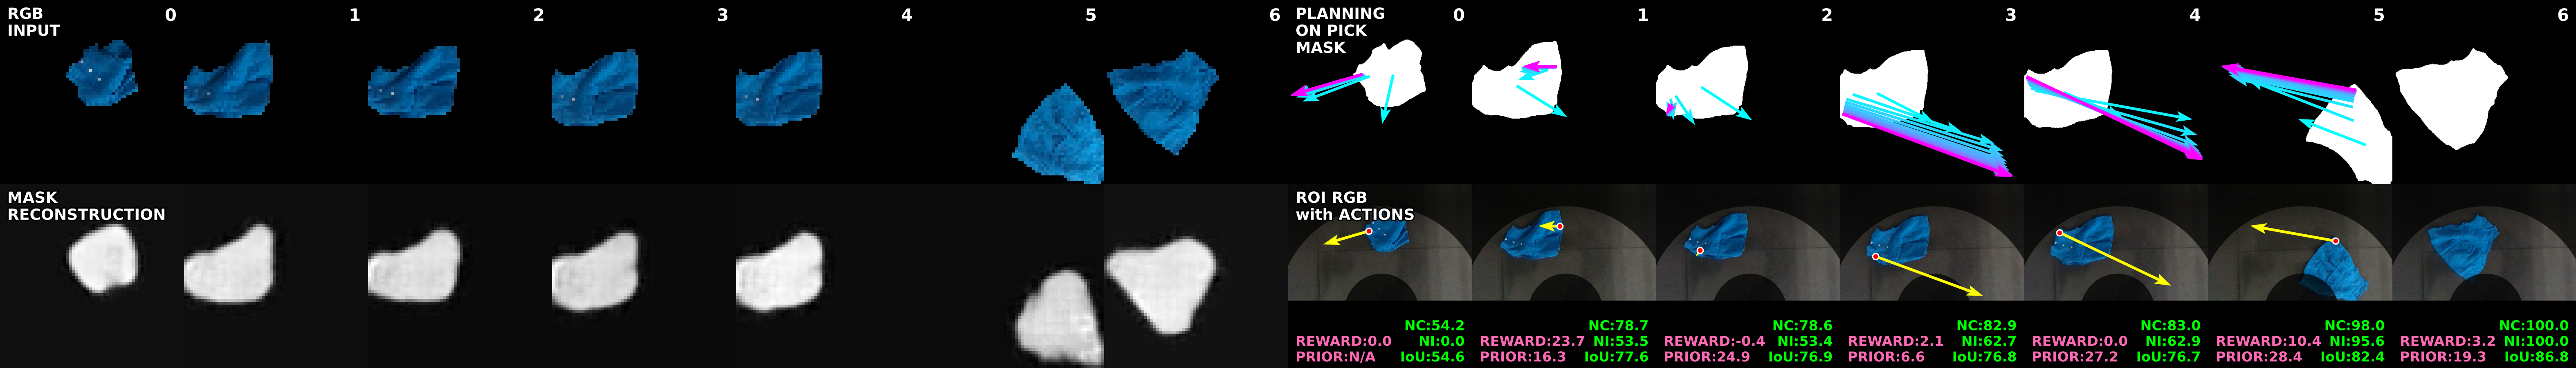
\includegraphics[width=1.0\linewidth]{plots/episode_4_combined.png}
        \end{minipage}
    }
    
    % Overall Figure Caption
    \caption{Overview of LaGarNet. (a) Initial and goal states of the simulated \text{Cloth3D} garments \cite{bertiche2020cloth3d}. (b) Real garments used for physical evaluation, where the shape and material of the yellow dress are out-of-distribution. (c) The UR5e real-world setup with an OnRobot RG2 gripper; input images are taken by a top-down RealSense camera. (d) LaGarNet flattening a real dress: bright blue arrows are the mean of the action Gaussian in the early CEM iterations and purple arrows the resulting final ones (top); the bottom row reports normalised coverage (NC), maximum IoU, the ground-truth reward and the prior reward predicted at the last planning step, all multiplied by 100. Trained in simulation \cite{canberk2023cloth}, LaGarNet transfers zero-shot to the real world for garment flattening.}
    \label{fig:LaGarNet}
\end{strip}

\begin{abstract} Manipulating cloth is a grand challenge in robotics: its many degrees of freedom yield an enormous state-action space that makes learning-based control extremely difficult to train. We present a goal-conditioned recurrent state-space model (GC-RSSM) that learns the latent dynamics of pick-and-place garment manipulation. Unlike the velocity- and position-controlled settings in which latent world models are usually studied, high-level pick-and-place is quasi-static: consecutive observations are not temporally continuous, and each transition is a single large deformation. We show that a recurrent latent world model nonetheless learns useful dynamics in this regime, and that our method LaGarNet matches the state-of-the-art performance of mesh-based methods on the difficult task of garment flattening whilst using five times fewer parameters and inferring over an order of magnitude faster---the first successful application of state-space models to complex garments. LaGarNet trains on our coverage-alignment reward and on our generalisable data collection procedure, producing a single policy that flattens four garment types in both simulation and the real world.
\end{abstract}

\begin{IEEEkeywords}
Robot Learning, Cloth Manipulation, World Model, Model-Based Reinforcement Learning
\end{IEEEkeywords}



\section{Introduction} \label{sec:introduction}

Robotic manipulation of cloth-like deformable objects is a significant technical challenge with profound societal and economic implications. Automating it is essential for modernising garment manufacturing \cite{nayak2018introduction}, for assisting elderly and mobility-impaired populations \cite{WHOaged2024, disablity2011world}, for domestic laundry, and for sterile handling in clinical settings \cite{cornish2021clinical}. Cloth manipulation remains difficult due to the complex, underactuated dynamics of cloth. Garment flattening is a foundational milestone preceding tasks such as folding, ironing and pressing \cite{doumanoglou2016folding}.

Data-driven garment flattening is dominated by two families. Behaviour cloning (BC) is conceptually simple, but the space of crumpled configurations is vast and covering it demands an impractical volume of human demonstrations \cite{weng2022fabricflownet, lips2024learning, huang2025sis}; BC flatteners therefore depend on scripted oracles or narrow their scope to a single garment type. Reinforcement learning (RL) explores that distribution directly in simulation, which is why most general flattening controllers are trained this way \cite{matas2018sim, lin2020softgym, canberk2023cloth, gu2023learning, ha2022flingbot}---and almost always with model-free algorithms. Model-based RL, which learns and exploits a world model of the environment \cite{ha2018world, hafner2019learning}, remains rare on garments: cloth's large degrees of freedom make such controllers extremely difficult to train \cite{kadi2023data}, and accurate world models have stayed elusive because of deformation and self-occlusion \cite{ma2021learning,yan2021learning,lin2020softgym}.

In our experiments, we adopt a top-down camera view and a single-gripper pick-and-place (PnP) primitive. Our human-in-the-loop experiments show operators flatten diverse garments exceptionally well with single-arm commands alone, indicating the primary bottleneck is physical reasoning rather than hardware. Restricting ourselves to one gripper isolates this challenge and focuses the work on representation learning, bypassing the complexities of bimanual coordination and multi-primitive control \cite{canberk2023cloth} at the cost of more iterations.

We present LaGarNet, a general single-policy method capable of flattening complex garment types (Figure \ref{fig:LaGarNet}). It mitigates the strong inductive biases of previous data-driven cloth manipulation methods \cite{kadi2025draper, weng2022fabricflownet, hoque2022visuospatial}, which rely on domain-specific architectures, reward functions and datasets from a particular blend of expert and random oracle policies, and generalise poorly since each garment type needs its own engineered oracle. LaGarNet instead couples a goal-conditioned recurrent state-space model (GC-RSSM) with a general data-collection procedure supported by an expert proximal Diffusion Policy \cite{chi2023diffusionpolicy} and a coverage-alignment reward. 

\text{LaGarNet} flattens four types of complex garments across the whole workspace of a real robot arm (Figure \ref{fig:ur3e-real-action-inference}). It outperforms strong baselines such as PlaNet-ClothPick \cite{kadi2024planet} and Diffusion Policy \cite{chi2023diffusionpolicy} and, most importantly, matches the mesh-based planner MEDOR \cite{huang2022mesh} with 17$\times$ faster inference and 5$\times$ fewer parameters, planning in a compact latent space rather than over a mesh. It is also competitive with human operators under the same single-arm constraint, although humans retain the highest success rate at long horizons. Transferred zero-shot, it averages 90\% NC, 80\% NI and 81\% Max IoU on the real garments of Figure \ref{fig:real-garments}. We make four contributions:

1. We propose a goal-conditioned recurrent state-space model (GC-RSSM) and show that a recurrent latent world model is effective in the \emph{quasi-static} pick-and-place regime, where consecutive frames are not temporally continuous, enabling \text{LaGarNet} to flatten garments in simulation and the real world at a fraction of the parameter count and inference cost of mesh-based world models.

2. We develop a data-collection strategy for offline \text{PnP} garment flattening, mixing a \text{Diffusion Policy} expert learned from few demonstrations with a mask-biased random policy.

3. We design a coverage-alignment reward for garment flattening, computable in both simulation and the real world.

4. We develop a transfer heuristic adapting the policy from a square observation window to a ring-shaped robot workspace.

% Apart from the introduction (Section \ref{sec:introduction}) and the conclusion (Section \ref{sec:conclusion}), the remainder of this paper is organised as follows. Section \ref{sec:related-workd} presents the state-of-the-art development of garment flattening in robotics. Section \ref{sec:planet-clothpick++} details the proposed method, \text{LaGarNet}. Section \ref{sec:transfer-heuristic} describes the transfer heuristic employed to bridge the gap between simulation and real-world observation-action space. Section \ref{sec:experiments} presents both simulation, real-world experimental results and a set of detailed ablation studies, along with corresponding analyses. Finally, Section \ref{sec:discussion} addresses the current limitations of our approach and outlines potential directions for future research.


\section{Related Work} \label{sec:related-workd}


\noindent Learning-based methods for cloth-shaping tasks, i.e., flattening and folding cloth-like objects, span \text{model-free reinforcement learning} \cite{matas2018sim,lin2020softgym,lee2021learning, canberk2023cloth, gu2023learning, avigal2022speedfolding}, \text{model-based reinforcement learning} \cite{yan2021learning,hoque2022visuospatial,ma2021learning,arnold2023cloth,lin2022learning, huang2022mesh} and \text{behaviour cloning} \cite{lips2024learning,weng2022fabricflownet, mo2022foldsformer, huang2025sis, chi2023diffusionpolicy}. Many successful controllers rely on intermediate explicit representations to mitigate the severe self-occlusion problem of cloth: key-point detection \cite{lips2024learning}, seam feature extraction \cite{huang2025sis}, mesh reconstruction \cite{huang2022mesh}, optical flow \cite{weng2022fabricflownet} and dense visual correspondence between current and goal images \cite{wu2024unigarmentmanip}. In contrast, we learn a latent dynamic representation and generate actions through planning, which makes our method generalisable to different scenarios.

These systems also vary in action space. Some attempt low-level position/velocity control \cite{matas2018sim,lin2020softgym}, whilst others adopt \text{pick-and-fling} (PnF) \cite{doumanoglou2014autonomous}, \text{pick-and-place} (PnP) \cite{sun2015accurate} or \text{pick-and-drag} (PnD) \cite{he2024fabricfolding} primitives. Hybrids of these three primitives are highly effective for diverse garment manipulation \cite{avigal2022speedfolding, canberk2023cloth}, but complicate both data collection and control. Single-gripper PnP suffers only from misgrasping, multi-layer grasping and cloth slipping \cite{lin2022learning, hoque2022visuospatial}, which have been addressed from both hardware and control perspectives \cite{kadi2025draper}. We therefore focus on PnP primitives and on the learning aspects of the latent dynamic model.

\subsection{Model-Based Methods in Cloth Shaping} \label{sec:mbrl}

Cloth dynamics are prevalent in reinforcement learning: learning and using them improves the data efficiency of policy training and the precision of actions at inference time \cite{hafner2019learning, kadi2024planet, lin2022learning}, and is effective for goal-conditioned tasks \cite{duan2024learning, hoque2022visuospatial}, where the distance between current and goal states can be exploited for planning. Model-based methods in this domain are either mesh-based or mesh-free, depending on whether a cloth mesh is reconstructed at test time.

Most model-based methods reconstruct a 3D mesh and its dynamics for the target cloth \cite{huang2022mesh, lin2022learning}. \text{Visible Connectivity Dynamics (VCD)} \cite{lin2022learning} first applies such a mesh model to the visible part of the cloth for more precise planning. Building on VCD, Huang et al.~\cite{huang2022mesh} adopt point clouds as input for mesh reconstruction and planning in the mesh-dynamic space; their method \text{MEDOR} explicitly reconstructs the occluded part of the cloth from a top-down camera by fine-tuning an initial mesh in real time against a template of the target garment. 

Among mesh-free approaches, \text{Contrastive Forward Modelling (CFM)} \cite{yan2021learning} trains latent dynamics for planning, and Hoque et al.~\cite{hoque2022visuospatial} propose \text{Visual Foresight Modelling (VSF)}, integrating variational video prediction models within the \text{Visual MPC} framework \cite{ebert2018visual} to address model exploitation. VSF nevertheless shows limited efficacy in garment flattening, and neither mesh-free planner has matched mesh-based VCD \cite{lin2022learning}. In contrast, our mesh-free planning method \text{LaGarNet} matches the state-of-the-art performance of the above mesh-based methods on flattening whilst using fewer parameters and inferring faster.

The mesh-free \text{Deep Planning Network (PlaNet)} \cite{hafner2019learning} is widely studied in control tasks \cite{yan2021learning, ma2021learning, lin2020softgym}, but shows limited efficacy on deformable objects, attributed to blurred visual reconstructions that lose the edge and corner details critical for shaping \cite{yan2021learning, lin2022learning}. \text{PlaNet-ClothPick} \cite{kadi2024planet}, a cloth-flattening algorithm based on a recurrent state-space model (RSSM), mitigates this by restricting pick actions to the cloth mask, a flattening-specific reward and an engineered offline dataset; it achieves perfect flattening in simulation and over 70\% NC on real towels \cite{kadi2024planet, kadi2025draper}, but fails to generalise to complex garments because of these inductive biases. Our single-policy \text{LaGarNet} reduces them through a general data-collection procedure and a coverage-alignment reward.

Model-based methods derive rewards from the difference between current and goal observations \cite{hoque2022visuospatial, yan2021learning}. Arnold et al.~\cite{arnold2023cloth} extend this to mesh-level goal-conditioned policies limited to fabrics. Model-free approaches train goal-conditioned representations \cite{mo2022foldsformer}, flow networks \cite{weng2022fabricflownet}, or use a \text{Hindsight Replay Buffer} \cite{andrychowicz2017hindsight, lee2021learning}, yet remain restricted to simple fabrics. We instead propose a goal-conditioned RSSM (GC-RSSM) predicting step-wise flattening rewards, which flattens longsleeved T-shirts, trousers, skirts and dresses.




\subsection{Reward Functions in Cloth Shaping} \label{sec:reward-literature}
Reward engineering is essential to the success of a reinforcement learning (RL) controller, and most garment-flattening systems come with their own reward function \cite{canberk2023cloth, gu2023learning, avigal2022speedfolding}. \text{ClothFunnels} \cite{canberk2023cloth} adopts a canonicalisation-alignment reward $\mathcal{R}_{NA} = \alpha\mathcal{R}_{dN} + (1-\alpha)\mathcal{R}_{dA}$, linearly interpolating a normalised delta deformation distance for alignment $\mathcal{R}_{dA}$ and a normalised delta rigid distance for canonicalisation $\mathcal{R}_{dN}$. \text{Learning2Unfold} \cite{gu2023learning} employs a similar interpolation between the normalised coverage $\mathcal{R}_C$ and an orientation term $\mathcal{R}_o = 1 - tanh^2\theta$, where $\theta = \alpha|\theta_P| + (1-\alpha)|\theta_F|$ combines the angle $\theta_P$ between current and goal cloth with the flipping angle $\theta_F$ that assures the cloth faces down. 


\text{SpeedFolding} \cite{avigal2022speedfolding} uses a coverage-smoothness reward $\mathcal{R}_{CS} = max(tanh(\alpha*\mathcal{R}_{dC} + \beta*\Tilde{R}_{dS}), 0)$, mixing the delta coverage $\mathcal{R}_{dC} = NC_t - NC_{t-1}$ with a delta smoothness estimate $\Tilde{R}_{dS}$ between the current and last frame, inferred by a pre-trained smoothness prediction network. \text{PlaNet-ClothPick} engineers a fabric-flattening reward based on \text{VSF}'s \cite{hoque2022visuospatial}. We propose a coverage-alignment reward $\mathcal{R}_{CA}$ that simplifies SpeedFolding's $\mathcal{R}_{CS}$ and, unlike ClothFunnels' canonicalisation-alignment reward, requires no particle-wise distances and hence no oracle, so it should in theory work for both simulation and real-world learning.

% \begin{figure}[t!]
%     \centering
%     \subfloat[\centering Human Policy Trajectory \label{fig:human-tshirt-demo}] {{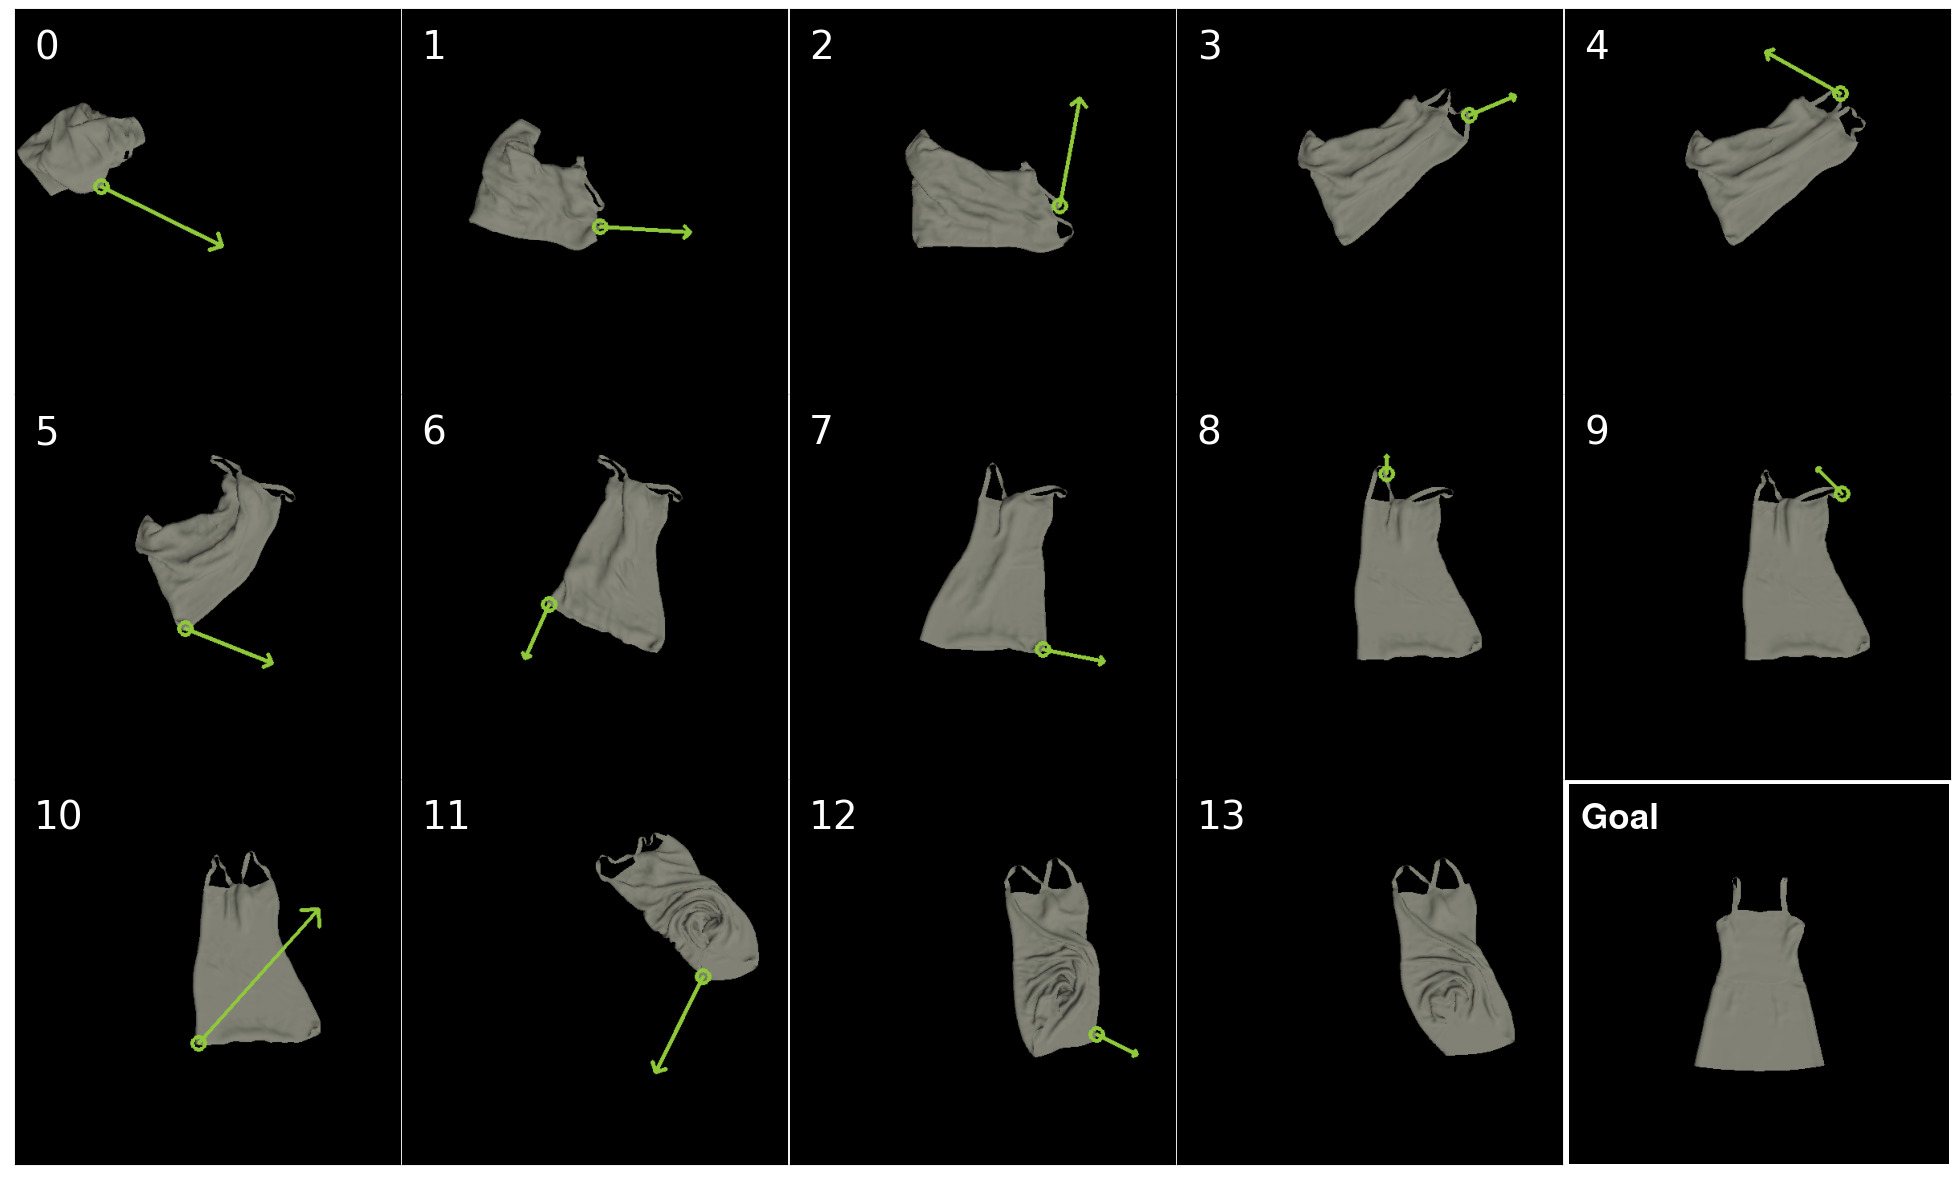
\includegraphics[width=0.27\textwidth]{plots/huam-trj-with-goal.jpg} }}
%     \subfloat[\centering Rewards \label{fig:reward-diff}] {{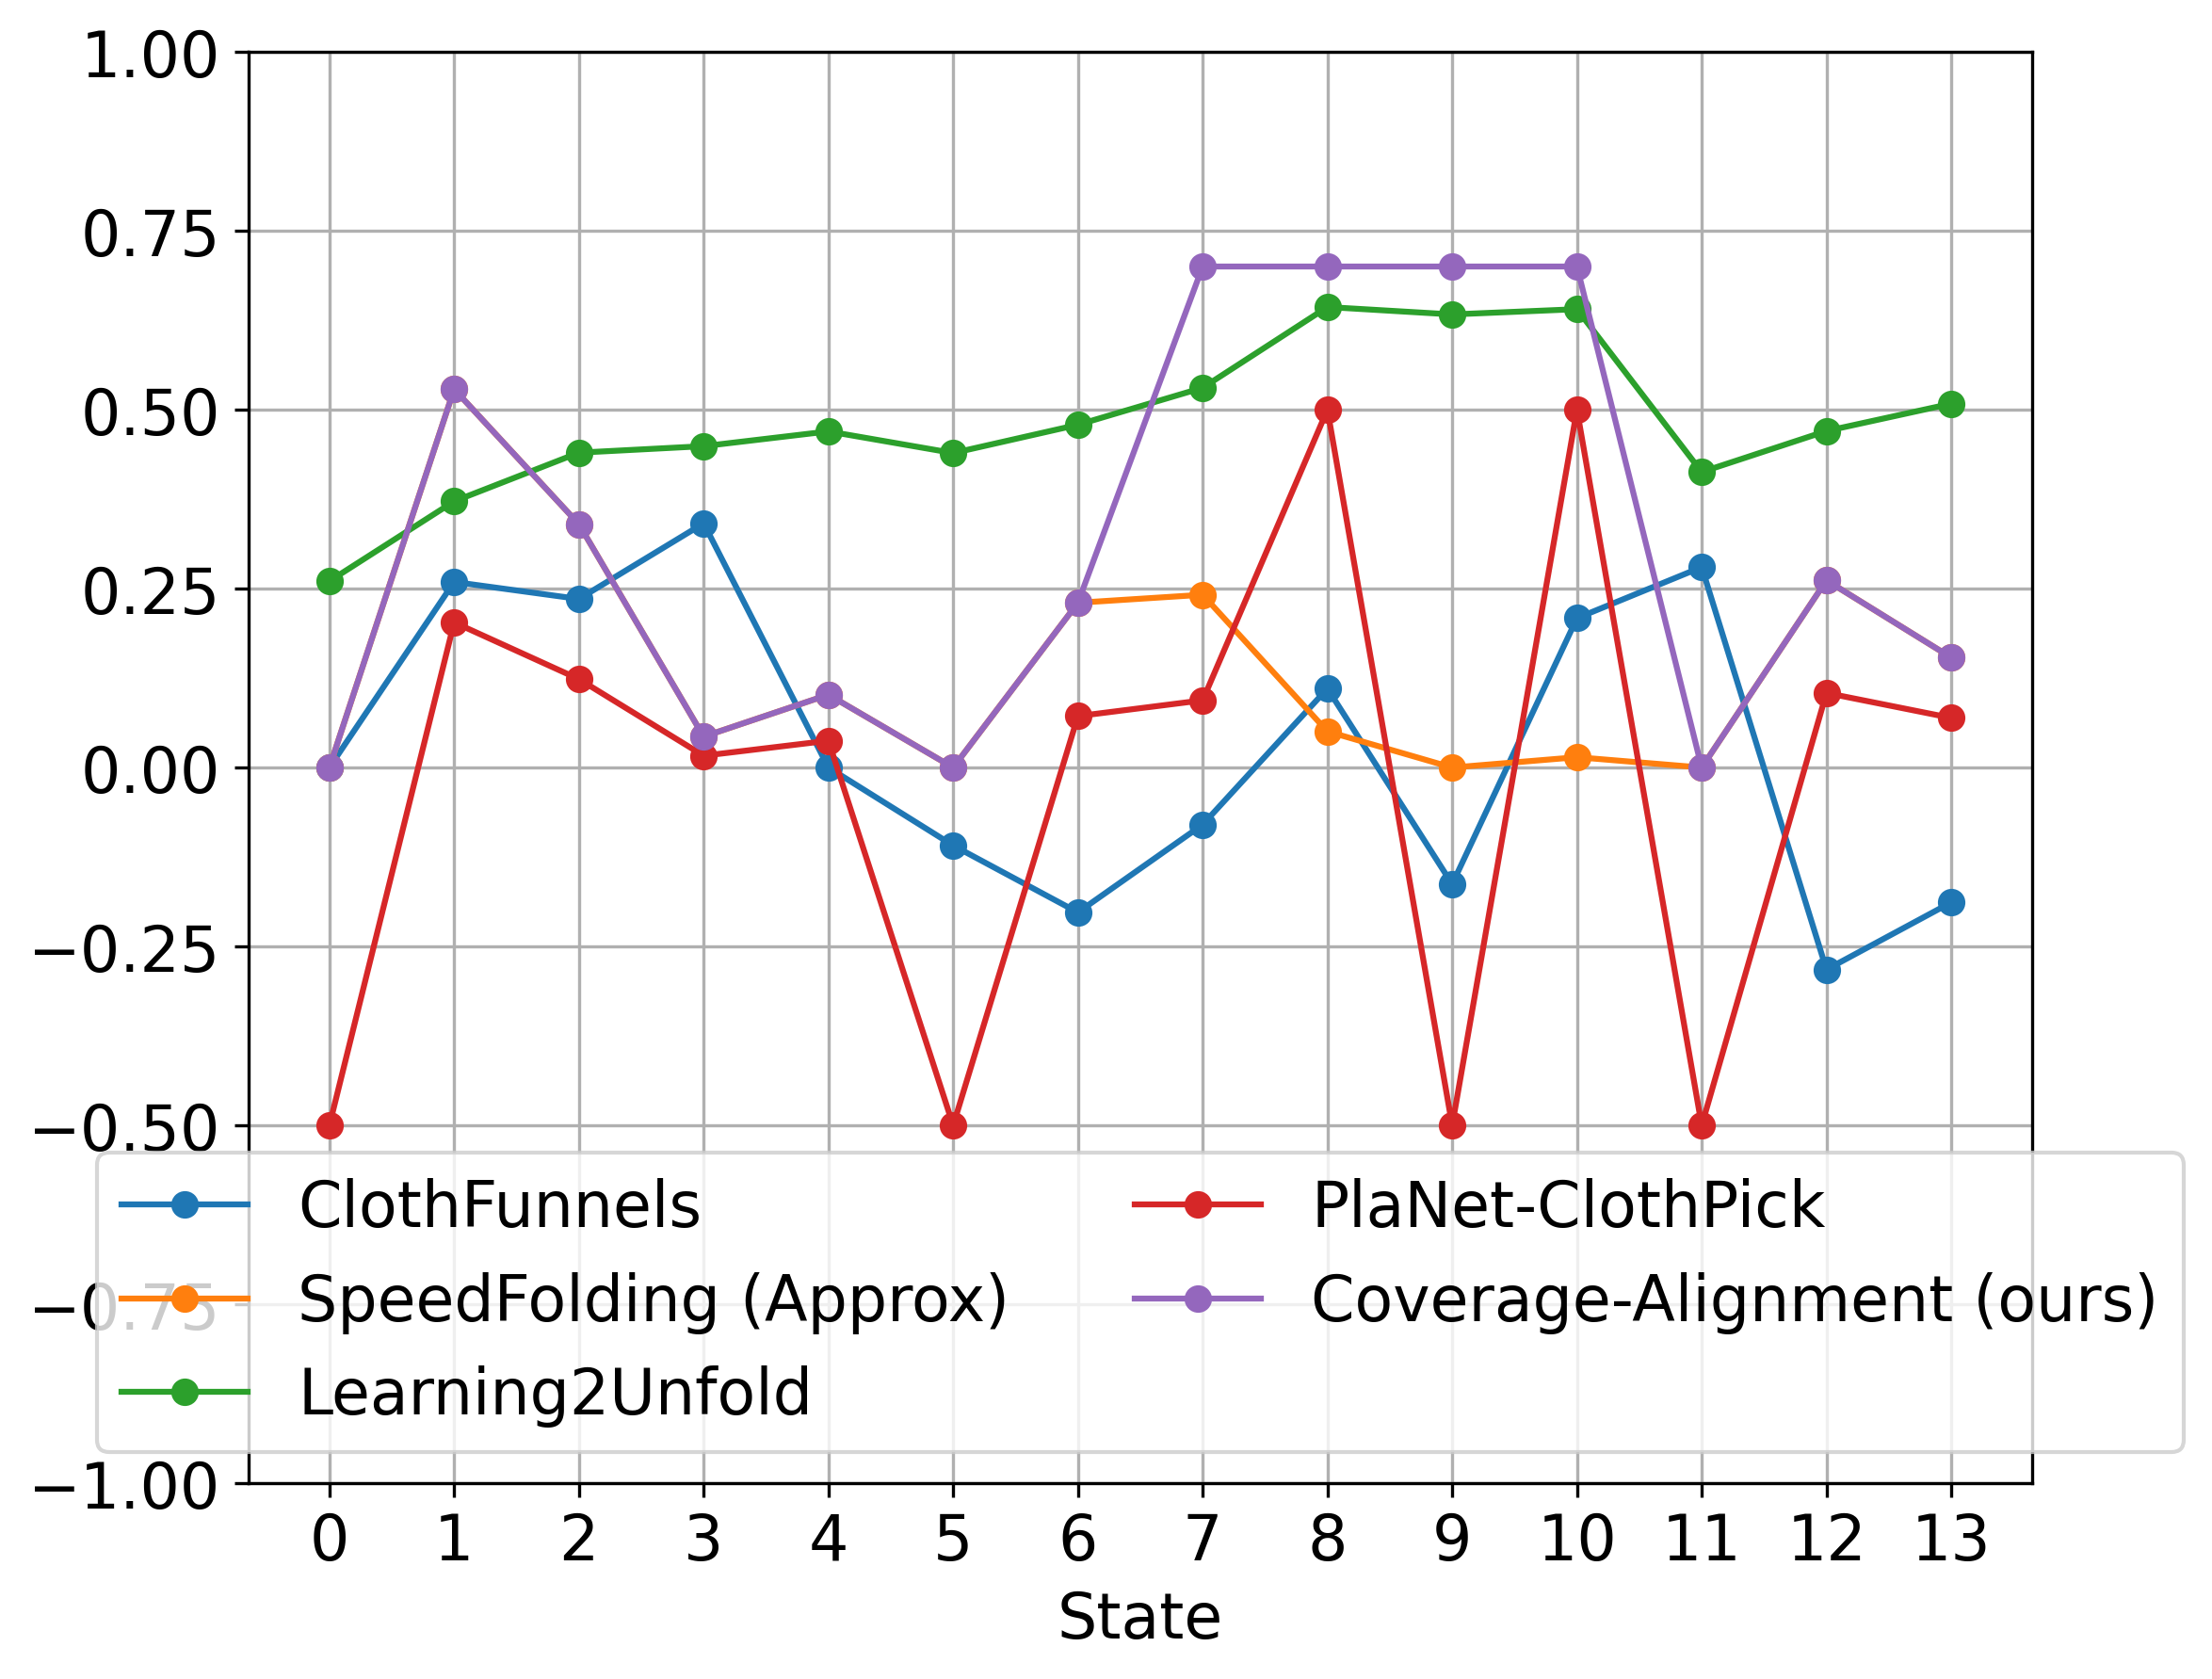
\includegraphics[width=0.22\textwidth]{plots/human-rewards.png} }}
%     \caption{Rewards of human policy in flattening a simulated dress. Figure (a) demonstrates the trajectory rollout of a human policy; Figure (b) shows the step-wise comparison of the reward function; and Figure (c) indicates the changes of different evaluation metrics for flattening. \texttt{SpeedFolding (Approx)} is the basis our initial coverage-alignment reward, where we use difference of Max IoU to replace the smoothness estimation. \texttt{Coverage-Alignment (ours)} is our final reward function with bonus and penality augmentaiton.}
% \end{figure}


\subsection{Data Collection and Preparation}

The high-dimensional state-action space of deformable objects makes policy representations, dynamics models and value functions hard to train, and model-based cloth-shaping methods further suffer from model exploitation (choosing actions the model incorrectly estimates as optimal) and compounding error in imagined roll-outs. A learned world model's effectiveness depends on how diverse and comprehensive the training trajectories are \cite{duan2024learning}, and training typically needs large amounts of data from carefully designed blends of policies \cite{hoque2022visuospatial, yan2021learning, kadi2024planet}. Prior work has used demonstration data \cite{matas2018sim}, corner-biased sampling that steers pick actions towards fabric corners and edges \cite{hoque2022visuospatial,weng2022fabricflownet}, and other engineered strategies \cite{arnold2023cloth,lin2022learning}---all of which impose strong inductive biases on the learning algorithm. We instead propose a general data collection procedure combining a Diffusion Policy \cite{chi2023diffusionpolicy} trained from a few human demonstrations with a random oracle policy, which empirically yields effective MBRL training data.


\subsection{Goal-Conditioned Methods using RSSM}
Previous research has integrated goal-conditioned learning into RSSMs. Pertsch et al.~\cite{pertsch2020long} propose a goal-condition predictor \text{(GCP)} conditioned on the initial and goal states of a subtask of a long-horizon task, improving planning with a hierarchical divide-and-conquer scheme that infers the action inversely from the current state and an optimised sub-goal. Duan et al.~\cite{duan2024learning} present the goal-directed exploration algorithm \text{MUN} and devise \text{GC-Dreamer} as a baseline, but condition its goal on the actor and critic networks instead of the world model. We instead condition the goal directly on the RSSM's latent state inference, which learns a better representation.



% \subsection{Action Inference in Cloth Shaping}


% Learning-based approaches using high-level action primitives for cloth-shaping tasks generally adopts two strategies to learn the action: continuous action inference and state-action value map.

% \subsubsection{Continuous Action Inference}
% Early vision-based learning methods for continuous action inference, such as \cite{matas2018sim} and \cite{yan2021learning}, have studied many model-free reinforcement learning algorithms for pixel-based pick-and-place (\text{PnP}) action primitives on fabrics. One technique that leads to better \text{PnP} continuous action policy learning is the separation of the inference of pick and place positions; \cite{wu2020learning} suggest using \text{Maximum Value of Placing} that selects the best picking position after choosing the best placing position. \text{Diffusion Policy} \cite{chi2023diffusionpolicy} adapted to PnP domain \cite{kadi2025draper} with continuos action inference demonstrated a promising performance on towel flattening and folding in the real world. In this paper, we choose the diffusion policy as a candidate of imitation learning methods that uses continuos action inference. Research community have generally drifted toward discretised action-space using the following state-action value maps for further performance improvement on garments, as it facilitates effective masking of high-level action primitives.

% \subsubsection{State-Action Value Map} Discretising \text{PnP} action space is a common technique in cloth-shaping literature for model-free reinforcement learning  methods. A prevalent strategy for garment manipulation is using state-action value map (\text{SAVM}), where a convolutional auto-encoder produces value heatmaps on observation images. Lee et al.~\cite{lee2021learning} first propose the use of \text{SAVM} in fabric manipulation tasks by rotating and scaling the observation image and stacking them channel-wise as input to a network. Their system, trained in the real world with goal-conditioned offline \text{Deep Q-Learning} \cite{mnih2013playing}, successfully achieves several fabric folding tasks. They examine six folding tasks, achieving perfect success rates for four easier folds but struggling with more complex ones. Building on this Rotate-Scale \text{SAVM} (RS-\text{SAVM}), \text{FlingBot} \cite{ha2022flingbot} employs dual robot arms for fling primitives, using online \text{RL} in simulation before fine-tuning in the real world with pre-collected data to enhance flattening performance. 

% Extending on \text{FlingBot}, \text{ClothFunnels} \cite{canberk2023cloth} introduces a canonicalised-alignment objective to align garments with a predefined configuration, combining \text{PnP} and \text{pick-and-fling} primitives via RS-\text{SAVM} decoders and corresponding encoders. \text{FabricFolding} \cite{he2024fabricfolding} further adds a \text{Pick-and-Drag} primitive, where one gripper stays stationary while the other performs a dragging motion, alongside a key-point detection network for transitioning from flattening to a heuristic folding policy \cite{canberk2023cloth}. Similarly, \text{Learning2Unfold} \cite{gu2023learning} builds on \text{ClothFunnels} using a key-point detection network to provide grasping masks for RS-\text{SAVM}s. Diverging from rotation-scaling channels, \text{SpeedFolding} \cite{avigal2022speedfolding} uses a \text{U-Net} \cite{ronneberger2015u} to generate \text{SAVM}s by directly predicting key pixel values for place, fling, and drag actions. Their system, trained with a hybrid of offline and online \text{RL}, achieves nearly 10x speed-up over prior works \cite{doumanoglou2016folding, maitin2010cloth}. 

% In contrast, \text{JA-TN} \cite{kadi2024mjtn}, a behaviour cloning method building on \text{TransporterNet} \cite{zeng2021transporter}, infers direct \text{SAVM} and demonstrates high performance on single-gripper \text{PnP} towel shaping in both simulation and the real world. DRAPER \cite{kadi2025draper} demonstrate that the real-world deployed \text{JA-TN} can achieve above 87\% \text{NC} and  82\% \text{NI} on flattening rectangular fabrics with various types of materials. In this paper, we also investigates the performance of \text{JA-TN} on complex garment flattening tasks. Also, we choose the off-the-shelf \text{ClothFunnels} as the reinforcement learning  representative that uses SAVM action inference.


\section{LaGarNet} \label{sec:planet-clothpick++}

\begin{figure*}[h!]
    \centering
    
    % ===== ROW 1: (a) | (c) =====
    \begin{subfigure}[t]{0.67\linewidth}
        \centering
        \scalebox{0.65}{\tikz{
 % ================== CUSTOM STYLES ==================
 \tikzset{
   half-half/.style={
     path picture={
       \fill[orange!40] (path picture bounding box.south west) rectangle (path picture bounding box.north);
       \fill[red!80] (path picture bounding box.south) rectangle (path picture bounding box.north east);
     }
   }
 }

 % ================== NODES ==================
 % We group the nodes by time step. 
 % All spacing has been increased by 1.5x for a wider layout.

 % ------ t = 0 (Initial State) ------
 \node[latent, minimum size=0.8cm, fill=orange!40] (z0) {$\boldsymbol{z}_0$};
 \node[latent, rectangle, minimum size=0.8cm, above=0.6cm of z0] (h0) {$\boldsymbol{0}$};
 \node[obs, minimum size=0.8cm, above=0.6cm of h0] (a0) {$\boldsymbol{a}_{\text{no-op}}$}; 
 
 % y1 and r1 directly under z0
 \node[latent, minimum size=0.8cm, below=0.6cm of z0, fill=blue!40] (y0) {$\boldsymbol{y}_1$};
 \node[latent, minimum size=0.8cm, below=0.25cm of y0, fill=blue!40] (r0) {$\boldsymbol{r}_1$};
 
 % ------ t = 1 ------
 \node[latent, minimum size=0.8cm, right=1.8cm of z0, half-half] (z1) {$\boldsymbol{z}_1$};
 \node[latent, rectangle, minimum size=0.8cm, above=0.6cm of z1] (h1) {$\boldsymbol{h}_{1}$};
 \node[obs, minimum size=0.8cm, above=0.6cm of h1] (a1) {$\boldsymbol{a}_1$}; 
 
 \node[latent, minimum size=0.8cm, below=0.6cm of z1, fill=blue!40] (y1) {$\boldsymbol{y}_1$};
 \node[latent, minimum size=0.8cm, below=0.25cm of y1, fill=blue!40] (r1) {$\boldsymbol{r}_1$};
 
 % g and x scaled to 0.35cm left
 \node[obs, minimum size=0.8cm, left=0.35cm of z1, fill=green!30] (g1) {$\boldsymbol{g}$};
 \node[obs, minimum size=0.8cm, left=0.35cm of y1, fill=purple!30] (x1) {$\boldsymbol{x}_1$};

 % ------ t = 2 ------
 \node[latent, minimum size=0.8cm, right=1.8cm of z1, half-half] (z2) {$\boldsymbol{z}_2$};
 \node[latent, rectangle, minimum size=0.8cm, above=0.6cm of z2] (h2) {$\boldsymbol{h}_{2}$};
 \node[obs, minimum size=0.8cm, above=0.6cm of h2] (a2) {$\boldsymbol{a}_2$}; 
 
 \node[latent, minimum size=0.8cm, below=0.6cm of z2, fill=blue!40] (y2) {$\boldsymbol{y}_2$};
 \node[latent, minimum size=0.8cm, below=0.25cm of y2, fill=blue!40] (r2) {$\boldsymbol{r}_2$};
 
 \node[obs, minimum size=0.8cm, left=0.35cm of z2, fill=green!30] (g2) {$\boldsymbol{g}$};
 \node[obs, minimum size=0.8cm, left=0.35cm of y2, fill=purple!30] (x2) {$\boldsymbol{x}_2$};

 % ------ t - 1 ------
 \node[latent, minimum size=0.8cm, right=1.8cm of z2, half-half] (zt) {$\boldsymbol{z}_{t-1}$};
 \node[latent, rectangle, minimum size=0.8cm, above=0.6cm of zt] (ht) {$\boldsymbol{h}_{t-1}$};
 \node[obs, minimum size=0.8cm, above=0.6cm of ht] (at) {$\boldsymbol{a}_{t-1}$}; 
 
 \node[latent, minimum size=0.8cm, below=0.6cm of zt, fill=blue!40] (yt) {$\boldsymbol{y}_{t-1}$};
 \node[latent, minimum size=0.8cm, below=0.25cm of yt, fill=blue!40] (rt) {$\boldsymbol{r}_{t-1}$};
 
 \node[obs, minimum size=0.8cm, left=0.35cm of zt, fill=green!30] (gt) {$\boldsymbol{g}$};
 \node[obs, minimum size=0.8cm, left=0.35cm of yt, fill=purple!30] (xt) {$\boldsymbol{x}_{t-1}$};

 % ------ t ------
 \node[latent, minimum size=0.8cm, right=1.8cm of zt, half-half] (zt1) {$\boldsymbol{z}_{t}$};
 \node[latent, rectangle, minimum size=0.8cm, above=0.6cm of zt1] (ht1) {$\boldsymbol{h}_{t}$};
 \node[latent, minimum size=0.8cm, above=0.6cm of ht1, fill=yellow!30] (at1) {$\boldsymbol{a}_{t}$}; 
 
 \node[latent, minimum size=0.8cm, below=0.6cm of zt1, fill=blue!40] (yt1) {$\boldsymbol{y}_{t}$};
 \node[latent, minimum size=0.8cm, below=0.25cm of yt1, fill=blue!40] (rt1) {$\boldsymbol{r}_{t}$};
 
 \node[obs, minimum size=0.8cm, left=0.35cm of zt1, fill=green!30] (gt1) {$\boldsymbol{g}$};
 \node[obs, minimum size=0.8cm, left=0.35cm of yt1, fill=purple!30] (xt1) {$\boldsymbol{x}_{t}$};

 % ------ t + 1 (No x node) ------
 \node[latent, minimum size=0.8cm, right=1.8cm of zt1, fill=red!80] (zt2) {$\boldsymbol{z}_{t+1}$};
 \node[latent, rectangle, minimum size=0.8cm, above=0.6cm of zt2] (ht2) {$\boldsymbol{h}_{t+1}$};
 \node[latent, minimum size=0.8cm, above=0.6cm of ht2, fill=yellow!30] (at2) {$\boldsymbol{a}_{t+1}$}; 
 
 \node[latent, minimum size=0.8cm, below=0.6cm of zt2, fill=blue!15] (yt2) {$\boldsymbol{y}_{t+1}$};
 \node[latent, minimum size=0.8cm, below=0.25cm of yt2, fill=blue!15] (rt2) {$\boldsymbol{r}_{t+1}$};
 
 \node[obs, minimum size=0.8cm, left=0.35cm of zt2, fill=green!30] (gt2) {$\boldsymbol{g}$};

 % ------ T (No x node) ------
 \node[latent, minimum size=0.8cm, right=1.8cm of zt2, fill=red!80] (zT) {$\boldsymbol{z}_T$};
 \node[latent, rectangle, minimum size=0.8cm, above=0.6cm of zT] (hT) {$\boldsymbol{h}_{T}$};
 \node[latent, minimum size=0.8cm, above=0.6cm of hT, fill=yellow!30] (aT) {$\boldsymbol{a}_{T}$}; 
 
 \node[latent, minimum size=0.8cm, below=0.6cm of zT, fill=blue!15] (yT) {$\boldsymbol{y}_{T}$};
 \node[latent, minimum size=0.8cm, below=0.25cm of yT, fill=blue!15] (rT) {$\boldsymbol{r}_{T}$};
 
 \node[obs, minimum size=0.8cm, left=0.35cm of zT, fill=green!30] (gT) {$\boldsymbol{g}$};

 % ================== EDGES ==================

 % 1. Generation of h (ORANGE)
 \edge[black, very thick] {a0, h0, z0} {h1} 
 \edge[black, very thick] {a1, h1, z1} {h2} 
 \edge[black, very thick] {at, ht, zt} {ht1} 
 \edge[black, very thick] {at1, ht1, zt1} {ht2}
 
 % 2. Generation of y and r (BLUE)
 % Vertical edges
 \edge[blue, very thick] {z0}{y0} \edge[blue, very thick] {z1}{y1} \edge[blue, very thick] {z2}{y2} 
 \edge[blue, very thick] {zt}{yt} \edge[blue, very thick] {zt1}{yt1} \edge[blue, very thick] {zt2}{yt2} \edge[blue, very thick] {zT}{yT}
 
 % Curved edges
 \path (z0) edge [bend left=45, ->, blue, very thick] (r0); \path (h0) edge [bend left=45, ->, blue, very thick] (y0); \path (h0) edge [bend left=45, ->, blue, very thick] (r0);
 \path (z1) edge [bend left=45, ->, blue, very thick] (r1); \path (h1) edge [bend left=45, ->, blue, very thick] (y1); \path (h1) edge [bend left=45, ->, blue, very thick] (r1);
 \path (z2) edge [bend left=45, ->, blue, very thick] (r2); \path (h2) edge [bend left=45, ->, blue, very thick] (y2); \path (h2) edge [bend left=45, ->, blue, very thick] (r2);
 \path (zt) edge [bend left=45, ->, blue, very thick] (rt); \path (ht) edge [bend left=45, ->, blue, very thick] (yt); \path (ht) edge [bend left=45, ->, blue, very thick] (rt);
 \path (zt1) edge [bend left=45, ->, blue, very thick] (rt1); \path (ht1) edge [bend left=45, ->, blue, very thick] (yt1); \path (ht1) edge [bend left=45, ->, blue, very thick] (rt1);
 \path (zt2) edge [bend left=45, ->, blue, very thick] (rt2); \path (ht2) edge [bend left=45, ->, blue, very thick] (yt2); \path (ht2) edge [bend left=45, ->, blue, very thick] (rt2);
 \path (zT) edge [bend left=45, ->, blue, very thick] (rT); \path (hT) edge [bend left=45, ->, blue, very thick] (yT); \path (hT) edge [bend left=45, ->, blue, very thick] (rT);

 % 3. Inference of z (RED, DASHED)
 % Inference from g
 \path (g1) edge [densely dashed, bend left=25, ->, orange, very thick] (z0); 
 \path (g1) edge [densely dashed, bend left=25, ->, orange, very thick] (z1);
 \path (g2) edge [densely dashed, bend left=25, ->, orange, very thick] (z2);
 \path (gt) edge [densely dashed, bend left=25, ->, orange, very thick] (zt);
 \path (gt1) edge [densely dashed, bend left=25, ->, orange, very thick] (zt1);

 % Inference from x 
 \path (x1) edge [densely dashed, bend left=15, ->, orange, very thick] (z0); 
 \path (x1) edge [densely dashed, bend left=15, ->, orange, very thick] (z1);
 \path (x2) edge [densely dashed, bend left=15, ->, orange, very thick] (z2);
 \path (xt) edge [densely dashed, bend left=15, ->, orange, very thick] (zt);
 \path (xt1) edge [densely dashed, bend left=15, ->, orange, very thick] (zt1);

 % Inference from h
 \path (h0) edge [densely dashed, bend right=30, ->, orange, very thick] (z0);
 \path (h1) edge [densely dashed, bend right=30, ->, orange, very thick] (z1);
 \path (h2) edge [densely dashed, bend right=30, ->, orange, very thick] (z2);
 \path (ht) edge [densely dashed, bend right=30, ->, orange, very thick] (zt);
 \path (ht1) edge [densely dashed, bend right=30, ->, orange, very thick] (zt1);

 % 4. Generation of z (RED, SOLID)
 % Solid vertical edges h -> z
 \edge[red, very thick] {h1}{z1} \edge[red, very thick] {h2}{z2} \edge[red, very thick] {ht}{zt} \edge[red, very thick] {ht1}{zt1} \edge[red, very thick] {ht2}{zt2} \edge[red, very thick] {hT}{zT}
 
 % Solid vertical edges g -> z
 \path (g1) edge [->, red, very thick] (z1);
 \path (g2) edge [->, red, very thick] (z2);
 \path (gt) edge [->, red, very thick] (zt);
 \path (gt1) edge [->, red, very thick] (zt1);
 \path (gt2) edge [->, red, very thick] (zt2);
 \path (gT) edge [->, red, very thick] (zT);


 % ================== DOTTED GAPS ==================
 % Gap between 2 and t-1
 \path (a2) -- node {\dots} (at); \path (h2) -- node {\dots} (ht); 
 \path (r2) -- node {\dots} (rt);

 % Gap between t+1 and T
 \path (at2) -- node {\dots} (aT); \path (ht2) -- node {\dots} (hT); 
 \path (yt2) -- node {\dots} (yT); \path (rt2) -- node {\dots} (rT);
}}
        \caption{Probabilistic Graphical Model of GC-RSSM}
        \label{fig:gc-rssm-pgm}
    \end{subfigure}
    \setcounter{subfigure}{2}% keep column-major lettering: (c)
    \begin{subfigure}[t]{0.32\linewidth}
        \centering
        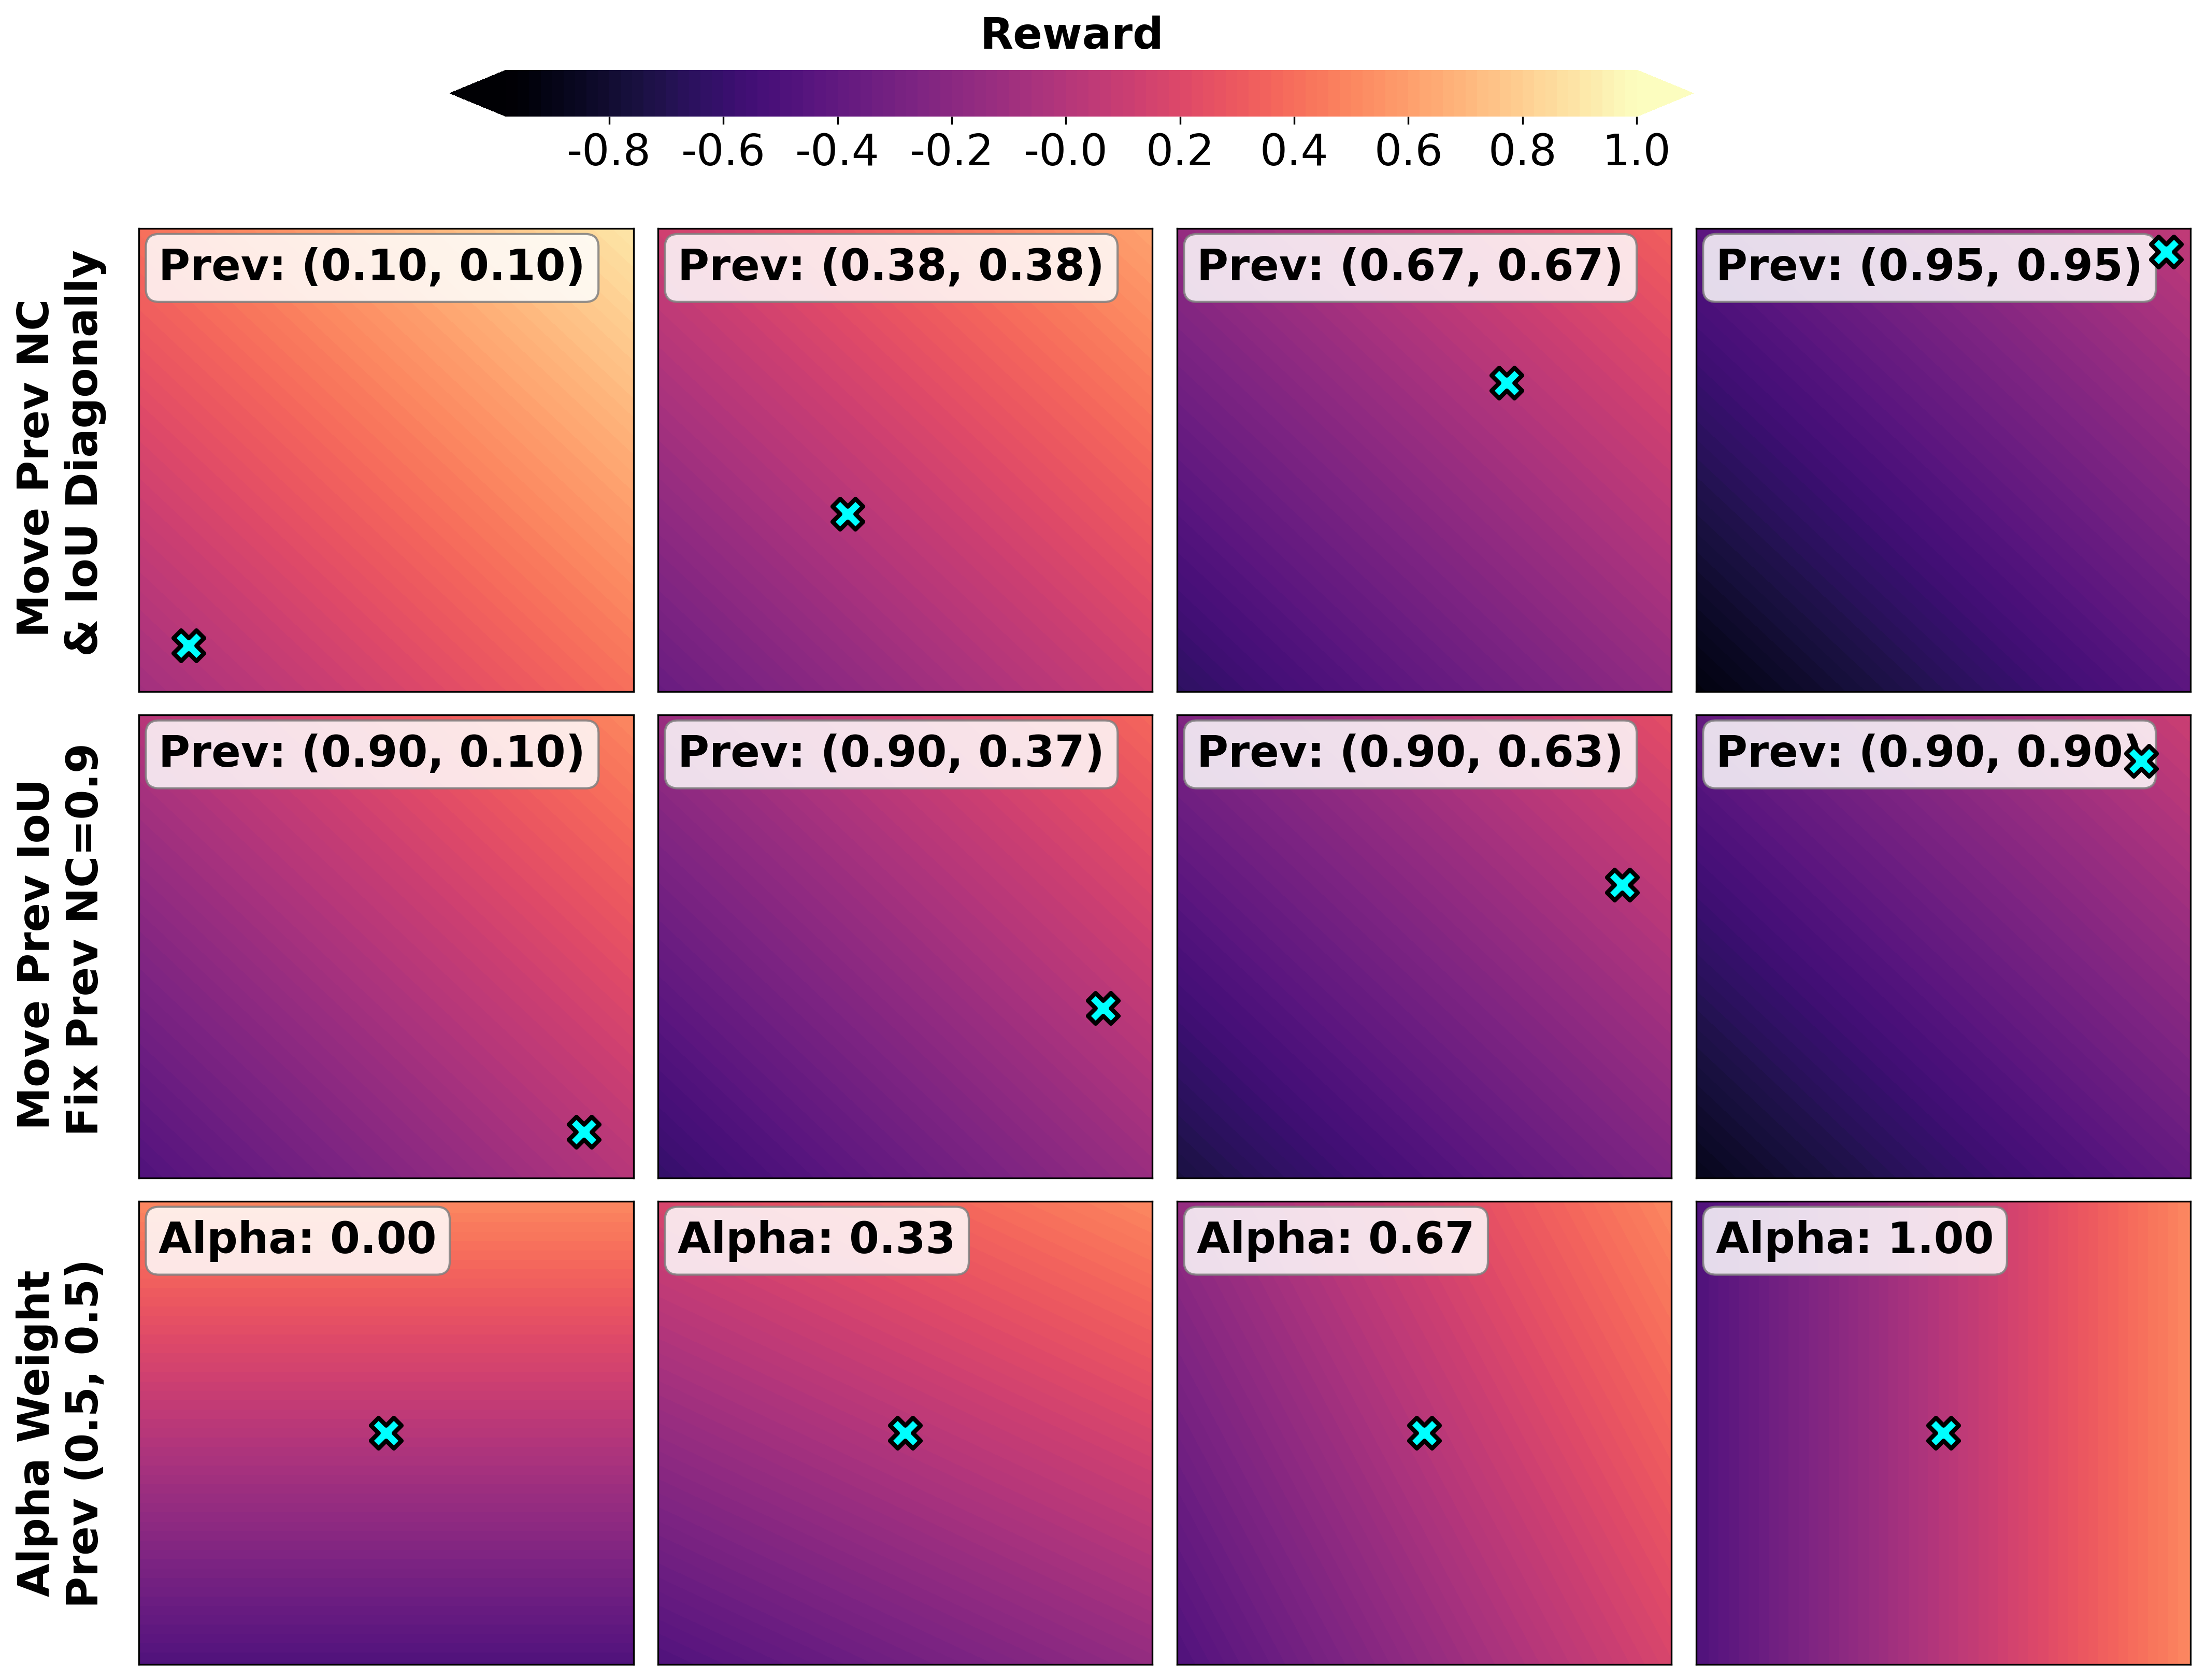
\includegraphics[width=\linewidth]{plots/reward_sensitivity_3x5.png}
        \caption{Coverage-Alignment Reward}
        \label{fig:reward-function}
    \end{subfigure}

    \vspace{6pt}

    % ===== ROW 2: (b) | (d) =====
    \setcounter{subfigure}{1}% (b)
    \begin{subfigure}[b]{0.67\linewidth}
        \centering
        \scalebox{0.60}{\tikz[
    >=stealth,
    % Standard rectangular block (kept original size for GRU)
    block/.style={rectangle, draw, thick, align=center, minimum height=1cm, minimum width=1.5cm, rounded corners=2pt},
    % NEW: Smaller MLP block
    mlpblock/.style={rectangle, draw, thick, align=center, minimum height=0.7cm, minimum width=1.1cm, rounded corners=2pt},
    % Narrower blocks specifically for the Z latents
    zblock/.style={rectangle, draw, thick, align=center, minimum height=0.8cm, minimum width=1.8cm, rounded corners=2pt},
    % Square blocks for images/goals (Empty fill for external labels)
    square/.style={rectangle, draw, thick, minimum size=2cm, fill=white},
    % Funnel shape style (for Encoders - compresses)
    funnel/.style={trapezium, draw, thick, trapezium stretches body, shape border rotate=270, minimum height=1.5cm, minimum width=1.2cm, fill=blue!10},
    % Funnel shape style (for Decoders - expands)
    dec_funnel/.style={trapezium, draw, thick, trapezium stretches body, shape border rotate=90, minimum height=1.5cm, minimum width=1.2cm, fill=blue!10},
    % Flat rectangular blocks for h and action
    flat/.style={rectangle, draw, thick, minimum height=0.6cm, minimum width=2cm, fill=white, align=center},
    % Slim rectangular blocks for 1D embeddings
    slim/.style={rectangle, draw, thick, minimum height=1.2cm, minimum width=0.4cm, fill=white, align=center},
    % Half split style for latent variables
    half split/.style={
        path picture={
            \fill[orange!40] (path picture bounding box.south west) rectangle (path picture bounding box.north);
            \fill[red!80] (path picture bounding box.south) rectangle (path picture bounding box.north east);
        }
    }
]{
    % ================== CORE STACK ==================
    % 1. Central GRU
    \node[block, fill=gray!60] at (0, 0) (gcrssm) {GRU};

    % 2. Action MLP (Above GRU)
    \node[mlpblock, fill=gray!60] at (0, 1.5) (actmlp) {MLP};

    % 3. Latent Z blocks (Above Action MLP, Narrow, Red/Orange)
    \node[zblock, fill=orange!40] at (0, 3) (zhat) {$\boldsymbol{\hat{z}}_{1...T}$};
    \node[zblock, fill=red!80] at (0, 4.5) (ztilde) {$\boldsymbol{\tilde{z}}_{1...T}$};

    % ================== MLPs & STATE (LEFT OF GRU) ==================
    % 4. MLPs for z blocks (Left of Z blocks)
    \node[mlpblock, fill=orange!40] at (-2.5, 3) (postmlp) {MLP};
    \node[mlpblock, fill=red!80] at (-2.5, 4.5) (priormlp) {MLP};

    % 5. h block (Moved to the LEFT of GRU, perfectly beneath the Latent MLPs)
    \node[flat] at (-2.5, 0) (h) {$\boldsymbol{h}_{1...T}$};

    % ================== JOINT MLP (RIGHT OF GRU) ==================
    % 6. Joint Decoding MLP
    \node[mlpblock, fill=blue!20] at (2, 0) (jointmlp) {MLP};

    % ================== INPUTS (FAR LEFT SIDE) ==================
    % Action block (Left of h, underneath the e blocks)
    \node[flat, fill=gray!20] at (-5.7, 1.5) (action) {$\boldsymbol{a}_{\text{no-op},1...{t-1}}$};
    \node[flat, fill=yellow!20] at (-5.7, 0.9) (action_samp) {$\boldsymbol{a}_{{t...T}}$};

    % Goal inputs & Embeddings (Y = 5) - Labels outside!
    \node[slim, fill=green!30, label={above:$\boldsymbol{e}^g$}] at (-5.7, 4.5) (eg_box) {};
    \node[funnel, left=0.2cm of eg_box, fill=gray!30] (cnng) {CNN};
    \node[square, left=0.2cm of cnng, fill=green!30, label={above:$\boldsymbol{g}$}] (g_box) {
\includegraphics[width=1.8cm, height=1.8cm]{plots/goal.jpg}};

    % Observation inputs & Embeddings (Y = 3) - Labels outside!
    \node[slim, fill=purple!30, label={above:$\boldsymbol{e}^x_{1...t}$}] at (-5.7, 2.5) (ex_box) {};
    \node[funnel, left=0.2cm of ex_box, fill=gray!30] (cnnx) {CNN};
    \node[square, left=0.2cm of cnnx, fill=purple!30, label={below:$\boldsymbol{x}_{1...t}$}] (x_box) {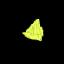
\includegraphics[width=1.8cm, height=1.8cm]{plots/input.jpg}};


    % ================== BIG GC-RSSM & Z BLOCKS ==================
    \begin{scope}[on background layer]
        % Group block surrounding zhat and ztilde - NOW TRANSPARENT
        \node[draw=purple!50, thick, fill=none, rounded corners=5pt, fit=(zhat) (ztilde), inner sep=0.2cm] (zgroup) {};

        % Coordinates to ensure the box pads well around the outer routing loops
        \coordinate (box_bottom) at (0, -1);
        \coordinate (box_left) at (-4.0, 0); 
        \node[draw=gray!80, ultra thick, dashed, fill=none, rounded corners=10pt, fit=(priormlp) (postmlp) (zgroup) (actmlp) (gcrssm) (h) (jointmlp) (box_bottom) (box_left), inner sep=0.42cm] (gcrssm_box) {};
        \node[above left, font=\bfseries, xshift=2.1cm, yshift=0cm, text=gray!80] at (ztilde.east) {GC-RSSM};
    \end{scope}


    % ================== OUTPUTS (FAR RIGHT SIDE) ==================
    % Decoders
    \node[mlpblock, fill=blue!40] at (4.3, 4) (decmlp) {MLP};
    \node[dec_funnel, fill=blue!40] at (4.3, 0) (deccnn) {CNN};

    % Reward Loss (Stacked on top of each other)
    \node[flat, minimum width=1.5cm, fill=blue!40] at (6.3, 4) (rhat) {$\boldsymbol{\hat{r}}_{1...T}$};
    \node[flat, minimum width=1.5cm, fill=blue!40] at (6.3, 5.5) (rgt) {$\boldsymbol{r}_{1...T}$}; 

    % Image Loss (Stacked on top of each other with labels on top and bottom)
    \node[square, label={below:$\boldsymbol{\hat{y}}_{1...T}$}, fill=blue!40] at (6.3, 0) (yhat) {
\includegraphics[width=1.8cm, height=1.8cm]{plots/recon.jpg}};
    \node[square, label={left:$\boldsymbol{y}_{1...T}$}, fill=blue!40] at (6.3, 2.5) (ygt) {
\includegraphics[width=1.8cm, height=1.8cm]{plots/output.jpg}};


    % ================== DATASET & AUGMENTATION (BOTTOM FAR LEFT) ==================
    % 1. Two side-by-side squares positioned below the x_box
    \node[square, below=1.4cm of x_box, xshift=0.6cm,label={below:$\boldsymbol{x}_\text{org}$}] (x_org) {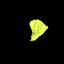
\includegraphics[width=1.8cm, height=1.8cm]{plots/original_obs.jpg}};
    \node[square, right=0.2cm of x_org,label={below:$\boldsymbol{g}_\text{org}$}] (goal_org) {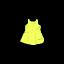
\includegraphics[width=1.8cm, height=1.8cm]{plots/original_goal.jpg}};

    % 2. The Dataset bounding box surrounding the two images
    \node[draw=gray!80, ultra thick, dashed, rounded corners=8pt, fit=(x_org) (goal_org), inner sep=0.4cm] (dataset_box) {};

    % 3. Arrow routing from the far left of the Dataset box to the far left of x_box
    \draw[->, ultra thick, dashed, black, rounded corners] (dataset_box.west) -- ++(-0.6, 0) |- node[pos=0.25, right, align=left, font=\footnotesize\bfseries] {Data Augmentation\\ (training only)} (x_box.west);

    \draw[->, ultra thick, dashed, black, rounded corners] (dataset_box.west) -- ++(-0.6, 0) |-  (g_box.west);
    
    % ================== ROUTING (Clean, 90-Degree Orthogonal) ==================

    % 1. Embeddings to Latent MLPs
    % Slightly offset vertical connection points to avoid line intersection
    \draw[->, ultra thick, red] ([yshift=0.2cm]eg_box.east) -- ([yshift=0.2cm]priormlp.west);
    \draw[->, ultra thick, dashed, orange] ([yshift=0.3cm]ex_box.east) -- ([yshift=-0.2cm]postmlp.west);
    
    % Goal embedding routes down cleanly into the Posterior MLP
    \draw[->, ultra thick, dashed, orange, rounded corners] (eg_box.east) -- ++(0.6,0) |- ([yshift=0.2cm]postmlp.west);

    % 2. MLPs to Latent States & KL Divergence (With Bell Curves!)
    \draw[->, ultra thick, red] (priormlp.east) -- node[above, yshift=2pt] {\tikz[scale=0.3]{\draw[thick] (-1.2,0) -- (1.2,0); \draw[thick, fill=red!80] (-1,0) .. controls (-0.5,0) and (-0.3,1.5) .. (0,1.5) .. controls (0.3,1.5) and (0.5,0) .. (1,0);}} (ztilde.west);
    
    \draw[->, ultra thick, dashed, orange] (postmlp.east) -- node[above, yshift=2pt] {\tikz[scale=0.3]{\draw[thick] (-1.2,0) -- (1.2,0); \draw[thick, fill=orange!40] (-1,0) .. controls (-0.5,0) and (-0.3,1.5) .. (0,1.5) .. controls (0.3,1.5) and (0.5,0) .. (1,0);}} (zhat.west);
    
    \draw[<->, ultra thick, purple, dashed] (ztilde.south) -- node[font=\bfseries] {KL Balance} (zhat.north);

    % 3. h feedback to Latent MLPs
    \draw[->, ultra thick, dashed, orange] (h.north) -- (postmlp.south);
    
    % Route h beautifully to the LEFT of the posterior mlp to reach priormlp
    \draw[->, ultra thick, red, rounded corners] (h.west) -- ++(-0.6, 0) |- ([yshift=-0.2cm]priormlp.west);

    % 4. Action & zhat into Action MLP
    \draw[->, ultra thick, solid, black] (zhat.south) -- (actmlp.north);
    
    % Action sneaks cleanly through a horizontal channel (crosses h-loop at a clean 90 degrees)
    \draw[->, ultra thick, black, rounded corners] (action.east) -- (actmlp.west);

    % 5. Action MLP output into GRU
    \draw[->, ultra thick, black] (actmlp.south) -- (gcrssm.north);

    % 6. GRU output to h, and h recurrent feedback
    \draw[->, ultra thick, black] (gcrssm.west) -- (h.east);
    % Feedback neatly loops left and underneath the GRU
    \draw[->, ultra thick, black, rounded corners] (h.south) -- ++(0,-0.55) -| (gcrssm.south);

    % 7. zgroup & h into Decoding Joint MLP
    % the new bounding box swoops beautifully to the right
    \draw[->, ultra thick, blue, rounded corners] (zgroup.east) -| (jointmlp.north);
    % h swoops beautifully completely under the GRU loop
    \draw[->, ultra thick, blue, rounded corners] ([xshift=-0.2cm]h.south) -- ++(0,-1.0) -| (jointmlp.south);

    % 8. Joint MLP to Decoders (Creates a neat rightward fork)
    \draw[->, ultra thick, blue, rounded corners] (jointmlp.east) -- ++(0.6,0) |- (decmlp.west);
    \draw[->, ultra thick, blue, rounded corners] (jointmlp.east) -- (deccnn.west);

    % 9. Decoders to Final Outputs and Losses (Arrows from decoders removed)
    % Vertical MSE loss arrow directly pointing from predicted to ground truth R
    \draw[<->, ultra thick, dashed, purple] (rhat.north) -- node[right, font=\bfseries] {MSE} (rgt.south);

    % Vertical MSE loss arrow directly pointing from predicted to ground truth Y
    \draw[<->, ultra thick, dashed, purple] (yhat.north) -- node[right, font=\bfseries] {MSE} (ygt.south);
}}
        \caption{Network Architecture and Training}
        \label{fig:network}
    \end{subfigure}
    \setcounter{subfigure}{3}% (d)
    \begin{subfigure}[b]{0.32\linewidth}
        \centering
        \scalebox{0.80}{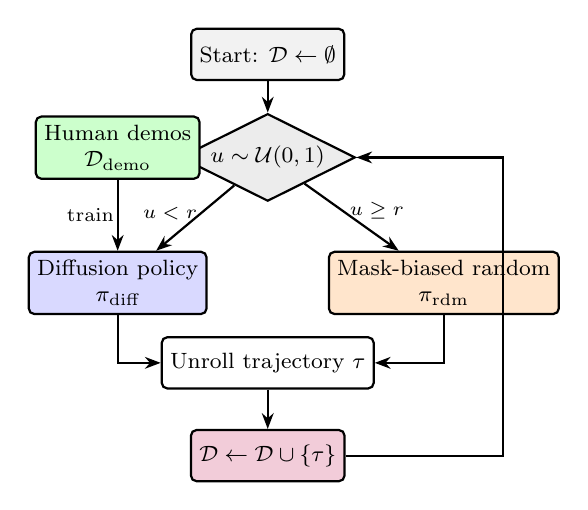
\begin{tikzpicture}[
            >={Stealth[length=2mm]},
            node distance=5mm,
            box/.style={rectangle, draw, thick, rounded corners=2pt, align=center,
                        inner sep=3pt, font=\footnotesize, minimum height=6.5mm},
            dec/.style={diamond, draw, thick, aspect=2, align=center,
                        inner sep=1pt, font=\footnotesize},
            lbl/.style={font=\scriptsize, inner sep=1pt}
        ]
            \node[box, fill=gray!10] (start) {Start: $\mathcal{D}\leftarrow\emptyset$};
            \node[dec, below=4mm of start, fill=gray!15] (dec) {$u\sim\mathcal{U}(0,1)$};
            \node[box, below left=9mm and 2mm of dec, fill=blue!15]  (diff) {Diffusion policy\\$\pi_{\text{diff}}$};
            \node[box, below right=9mm and 2mm of dec, fill=orange!20] (rdm) {Mask-biased random\\$\pi_{\text{rdm}}$};
            \node[box, above=9mm of diff, fill=green!20] (demo) {Human demos\\$\mathcal{D}_{\text{demo}}$};
            \node[box, below=17mm of dec, fill=white] (unroll) {Unroll trajectory $\tau$};
            \node[box, below=of unroll, fill=purple!20] (data) {$\mathcal{D}\leftarrow\mathcal{D}\cup\{\tau\}$};

            \draw[->, thick] (start) -- (dec);
            \draw[->, thick] (demo) -- node[lbl, left] {train} (diff);
            \draw[->, thick] (dec) -- node[lbl, above left=-1mm] {$u<r$} (diff);
            \draw[->, thick] (dec) -- node[lbl, above right=-1mm] {$u\geq r$} (rdm);
            \draw[->, thick] (diff) |- (unroll);
            \draw[->, thick] (rdm)  |- (unroll);
            \draw[->, thick] (unroll) -- (data);
            \draw[->, thick] (data.east) -- ++(20mm,0) |- (dec.east);
        \end{tikzpicture}}
        \caption{Data Collection Procedure}
        \label{fig:data-collection}
    \end{subfigure}

    % --- Main Overarching Caption ---
    \caption{LaGarNet: (a) the probabilistic graphical model and (b) the network architecture implementing it; matching colours, line styles, blocks and nodes denote identical processes. $\bm{g}$ is the goal observation, $\bm{x}_t$ and $\bm{z}_t$ the observation and latent state before action $\bm{a}_t$, and $\bm{h}_t$ the hidden state of the recurrent backbone. In (a), purple observation and grey action nodes are known model inputs, whereas yellow action nodes are sampled during planning. In (b), observation (purple) and goal (green) embeddings drive goal-directed dynamics, and a GRU (dark grey) updates the deterministic belief $\boldsymbol{h}$ from past actions processed by an MLP. The \textit{Prior} network (red, solid) predicts $\boldsymbol{\tilde{z}}$ from $\boldsymbol{h}$ and $\boldsymbol{g}$ alone, whilst the \textit{Posterior} network (orange, dashed) infers $\boldsymbol{\hat{z}}$ by additionally integrating $\boldsymbol{x}$, the two regularised by a balanced KL divergence. A joint decoder (blue) maps the deterministic and posterior latent states to the reconstruction $\boldsymbol{\hat{y}}$ and predicted reward $\boldsymbol{\hat{r}}$, both under MSE losses. (c) Sensitivity of the coverage-alignment reward $\mathcal{R}_{CA}$ to the interpolation coefficient $\alpha_r$. (d) The data-collection procedure: a Diffusion Policy trained on human demonstrations acts as the proximal expert and is mixed, at ratio $r$, with the mask-biased random policy to unroll the $M$ trajectories of the offline dataset $\mathcal{D}$.}
    \label{fig:lagarnet}
\end{figure*}

\text{LaGarNet} is an offline model-based deep reinforcement learning approach to garment flattening, trained on simulation data with domain randomisation (Figure \ref{fig:sim-train-init}) and transferred zero-shot to the real garments of Figure \ref{fig:real-garments}. It generalises by training a goal-conditioned recurrent state-space model (Section \ref{sec:gc-rssm}, Appendix \ref{sec:architecture}) on a coverage-alignment reward designed for all garment-flattening tasks (Section \ref{sec:ca-reward}), using a unified data collection procedure (Section \ref{sec:data-collection}) in which task-specific Diffusion Policies (Appendix \ref{sec:diffusion}) act as a proximal expert gathering trajectories around the successful distribution, plus data augmentation during training (Appendix \ref{sec:data-aug})---reaching state-of-the-art flattening performance with only 100 thousand interaction steps. The design takes inspiration from the working-memory literature in cognitive psychology: humans maintain and update task-relevant internal representations to infer hidden states from incomplete observations, predict future outcomes and plan towards a desired state \cite{miller2001integrative}. LaGarNet mirrors this with a goal-conditioned recurrent state-space model that maintains a belief state over the partially observed garment configuration, and a reward predictor that evaluates how candidate actions advance the task towards its goal \cite{hafner2019learning}.


\subsection{Goal-Conditioned Recurrent State Space Model} \label{sec:gc-rssm}


LaGarNet builds on State-Space Models (SSMs), generative frameworks for sequential data that support inferring future states and learning representations. Hafner et al.~\cite{hafner2019learning} define the Recurrent State-Space Model (RSSM) under the Partially Observable Markov Decision Process (POMDP) formulation, with latent state dynamics:
\begin{equation}
\begin{aligned}
    \text{Recurrent dynamic model:} & \quad \bm{h}_t=f(\bm{h}_{t-1},\bm{z}_{t-1},\bm{a}_{t-1}) \\
    \text{Representation model:}    & \quad \hat{\bm{z}}_t\sim q(\hat{\bm{z}}\;|\;\bm{h}_t,\bm{x}_t) \\
    \text{Transition predictor}    & \quad \tilde{\bm{z}}_t\sim p(\tilde{\bm{z}}\;|\;\bm{h}_{t}),
\end{aligned}
\end{equation}
where $\bm{x}$ represents the observation, $\bm{a}$ represents the action, $\bm{h}$ represents the deterministic latent representation, and ($\hat{\bm{z}}$, $\tilde{\bm{z}}$) represent the posterior and prior stochastic latent states. 

LaGarNet trains a goal-conditioned latent dynamics model by learning a feature representation $\bm{y}$, extending the RSSM with goal-conditioned inference and generation on the latent states (Figure~\ref{fig:gc-rssm-pgm}): the goal observation $\bm{g}$ enters the estimation of the stochastic latent representation $\bm{z}$, giving GC-RSSM as:

\begin{align}
    \hat{\bm{z}}_t &\sim q(\hat{\bm{z}} \;|\; \bm{h}_t, \bm{x}_t, \bm{g}) 
    && \text{GC Representation Model} \label{eq:gc-repr} \\
    \tilde{\bm{z}}_t &\sim p(\tilde{\bm{z}} \;|\; \bm{h}_t, \bm{g}) 
    && \text{GC Transition Predictor} \label{eq:gc-trans}
\end{align}



The training objective maximises the marginal log-likelihood of the estimated features and rewards given the action sequence and the target goal observation:
\begin{equation}
    \argmax_{\theta} \ln p(\bm{y}_{1:T}, r_{1:T} | \bm{a}_{1:T}, \bm{g}). \label{eqn:obj}
\end{equation}

Treating this as variational inference and optimising the Evidence Lower Bound (ELBO), the generative joint distribution and approximate posterior read:
\begin{align}
    &p(\bm{y}_{1:T}, r_{1:T}, \bm{z}_{1:T} | \bm{a}_{1:T}, \bm{g}) \nonumber \\
    &\quad = \prod_{t=1}^T p(\bm{y}_t|\bm{z}_t) p(r_t|\bm{z}_t) p(\bm{z}_t|\bm{z}_{t-1}, \bm{a}_{t-1}, \bm{g}) \label{eqn:rep-1}\\
    &q(\bm{z}_{1:T}| \bm{x}_{1:T}, \bm{a}_{1:T-1}, \bm{g}) = \prod_{t=1}^T q(\bm{z}_t| \bm{x}_{1:t}, \bm{a}_{1:t-1}, \bm{g}) \label{eqn:rep-2},
\end{align}
where we abstract the deterministic latent states $\bm{h}_t$ as they are directly computed from previous states. Expanding the objective in Equation \ref{eqn:obj} using the distributions in Equations \ref{eqn:rep-1} and \ref{eqn:rep-2}, we obtain the loss function (i.e., the evidence lower bound) of the GC-RSSM as:
\begin{align}
    \mathcal{L} =& \sum_{t=1}^{T} \mathbb{E}_{q(\bm{z}_{1:t-1})} \Bigg[ - 
     \underset{\bm{z}_t \sim q}{\E} \Big[ \ln p(\bm{y}_t|\bm{z}_t) + \ln p(r_t|\bm{z}_t) \Big] \nonumber\\
    &+ \text{KL}\Big[ q(\bm{z}_t|\bm{x}_{1:t}, \bm{a}_{1:{t-1}}, \bm{g}) \;\Big|\Big|\; p(\bm{z}_{t}|\bm{z}_{t-1}, \bm{a}_{t-1}, \bm{g}) \Big]
     \Bigg] \label{eqn:planet-objective-1}.
\end{align}

In our vision-based application the goal image $\bm{g} \in \mathbb{R}^{C\times H\times W}$ is processed by the same convolutional encoder as the current observation to produce the goal embedding $\bm{e}_g$, and the latent state $\bm{z}$ is sampled from the estimated Gaussians with the reparameterisation trick \cite{kingma2013auto} so gradients flow through it:
\begin{equation}
    \bm{z} = \bm{\mu} + \bm{\sigma} \odot \bm{\epsilon}, \quad \text{where } \bm{\epsilon} \sim \mathcal{N}(\bm{0}, \bm{I}) \label{eqn:reparam}
\end{equation}
To keep the standard deviation $\bm{\sigma}$ strictly positive and prevent numerical collapse, the raw variance output passes through a softplus, $f(x)=\ln(1+e^x)$, plus a minimum threshold $\sigma_{min}$.

Optimising the objective requires balancing its loss terms with scalar coefficients. We use MSE losses for feature and reward prediction (equivalent to the negative log-likelihood under a Gaussian), weighted by $\gamma_x$ and $\gamma_r$ in Equation \ref{eqn:total-loss}. For latent regularisation we adopt KL balancing \cite{hafner2021mastering}, scaling the prior and posterior gradients differently so the prior moves towards the posterior faster than vice versa, and we prevent posterior collapse with a ``free nat'' threshold $c$ (e.g., 1 nat) that clips the penalty below that divergence \cite{hafner2019learning}:
\begin{equation}
\begin{aligned}
    \mathcal{L}_{KL} = &\beta_{KL} \max\Big(c, \text{KL}\big[\text{sg}(q(\hat{\bm{z}}_t)) \;\big|\big|\; p(\tilde{\bm{z}}_t)\big]\Big) \\ 
    &+ (1 - \beta_{KL}) \max\Big(c, \text{KL}\big[q(\hat{\bm{z}}_t) \;\big|\big|\; \text{sg}(p(\tilde{\bm{z}}_t))\big]\Big)
\end{aligned} \label{eqn:kl-balance}
\end{equation}
where $\text{sg}(\cdot)$ is the stop-gradient operator and the term is scaled by $\gamma_{KL}$ in the total loss. To enforce consistent multi-step future predictions, we add overshooting losses---computed from more than one-step priors---on the KL divergence and reward predictions of future prior latent states across $T_f$ steps, weighted by $\gamma_{klo}$ and $\gamma_{ro}$. Table \ref{tab:all-hyperparameters} lists the exact coefficients.

During training we stop gradients only for the overshooting loss, never on the goals; GC-RSSM prevents the recurrent structure from ``forgetting'' the goal. The total loss is then:
\begin{equation}
    \mathcal{L}_{total} = \gamma_y \mathcal{L}_y + \gamma_r \mathcal{L}_r + \gamma_{KL} \mathcal{L}_{KL} + \gamma_{klo} \mathcal{L}_{klo} + \gamma_{ro} \mathcal{L}_{ro} \label{eqn:total-loss}
\end{equation}
where $\mathcal{L}_y$ and $\mathcal{L}_r$ are the MSE losses for feature and reward estimation and $\mathcal{L}_{klo}$, $\mathcal{L}_{ro}$ the corresponding overshooting losses over $T_f$ steps.

At test time LaGarNet takes $(\bm{x}_t, \bm{g})$ and maintains the posterior latent states $(\bm{h}_t, \hat{\bm{z}}_t)$, updating them with the previous action $\bm{a}_{t-1}$ and the current observation. Latent vectors start at zero, and the initial posterior states follow from applying a no-operation action $\bm{a}_{\text{no-op}}$:
\begin{equation}
    (\hat{\bm{z}}_0, \bm{h}_1) \sim \Big(q(\hat{\bm{z}}_0 \;|\; \bm{0}, \bm{x}_1, \bm{g}), f(\bm{0}, \hat{\bm{z}}_{0}, \bm{a}_{\text{no-op}})\Big).
\end{equation}
It then selects the first action $\bm{a}_t$ of a planned sequence of length $T_f$ by Model Predictive Control with the Cross-Entropy Method (MPC-CEM):
\begin{align}
   \bm{a}_{t:t+T_f-1} = \argmax_{\bm{a}} \sum_{k=t}^{t+T_f-1} r_\theta(\tilde{\bm{z}}_{k+1}(\bm{a}_k)),
\end{align}
where $\tilde{\bm{z}}_{k+1}(\bm{a}_k) \sim p(\tilde{\bm{z}}_{k+1} \;|\; \bm{h}_{k+1}=f(\bm{h}_k, \hat{\bm{z}}_k, \bm{a}_k), \bm{g})$. In our garment flattening setup, we set the prior future prediction horizon to $T_f=1$.

CEM solves this over the normalised action space $[-1,1]^4$, whose dimensions encode the pick and place positions in normalised pixel coordinates. The planner rejects, without resampling, any candidate whose pick pixel falls outside the intersection of the cloth mask and the robot's workspace mask, or whose place pixel falls outside the workspace mask, and executes the clipped mean of the final sampling distribution. Appendix~\ref{sec:planning} details the procedure and Appendix~\ref{sec:real-world-setup} the workspace mask and pixel-to-world conversion.
As shown in Figure \ref{fig:network}, LaGarNet comprises four components: a convolutional image encoder, a transposed-convolutional decoder, a goal-conditioned transition model built from MLPs and a Gated Recurrent Unit \cite{cho2014properties}, and a 5-layer MLP reward predictor, with ReLU activations throughout. Appendix \ref{sec:architecture} gives the layer configurations and Table \ref{tab:all-hyperparameters} the hyperparameters.

\subsection{Coverage-Alignment Reward}  \label{sec:ca-reward}

Our coverage-alignment reward $\mathcal{R}_{CA}$ combines the step-wise normalised coverage difference $\mathcal{R}_{dC}$ with the step-wise difference in maximum IoU between the current and goal cloth masks, $\mathcal{R}_{du}$: 

\begin{equation}
    \mathcal{R}_{CA} = \alpha_r \times\mathcal{R}_{dc} + (1-\alpha_r)\times \mathcal{R}_{du},
\end{equation}
where $\mathcal{R}_{dC} = \text{NC}_t - \text{NC}_{t-1}$ and $\mathcal{R}_{du} = \text{MaxIoU}_t - \text{MaxIoU}_{t-1}$; both $\mathcal{R}_{dC}$ and $\mathcal{R}_{du} \in [-1, 1]$, so that $\mathcal{R}_{CA} \in [-1, 1]$. In our experiments, we set $\alpha_r$ to 0.3 for our final LaGarNet. This reward function turns out to be easy to learn due to its continuous and linear nature.

% \begin{figure*}[t!]
%     \centering
%     \begin{subfigure}[t]{0.5\linewidth}
% 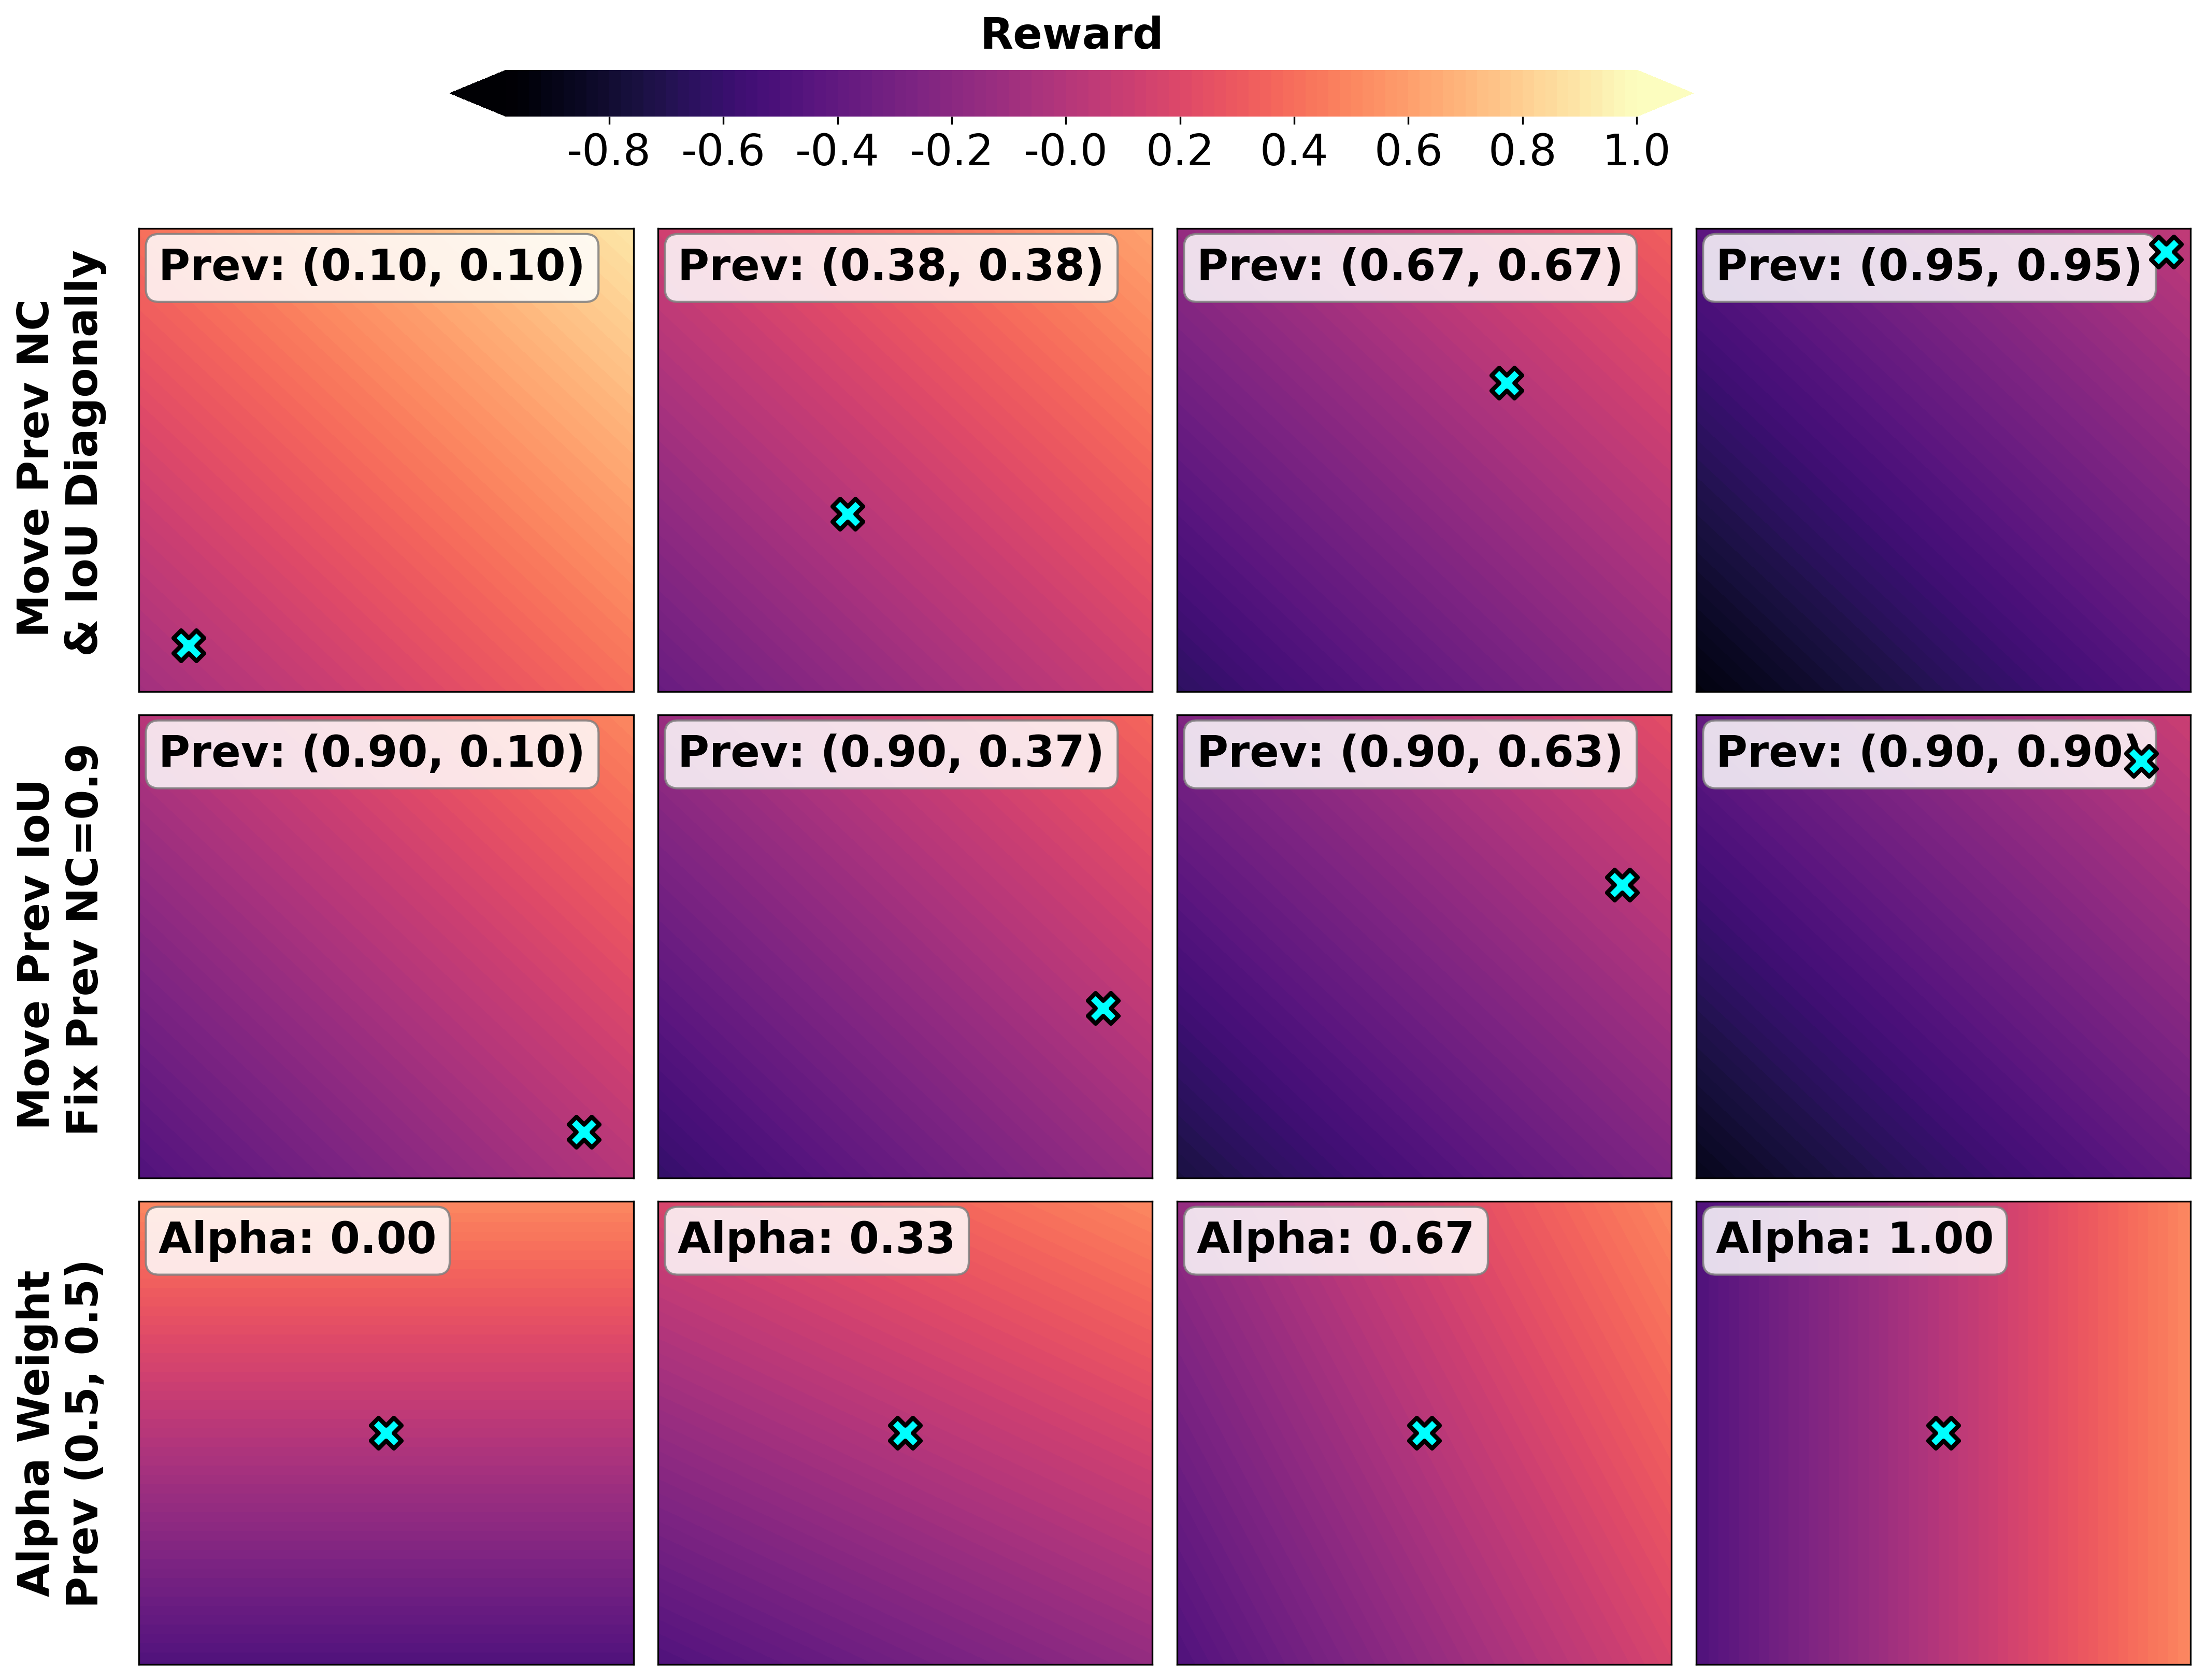
\includegraphics[width=\textwidth]{plots/reward_sensitivity_3x5.png}
%     \caption{Coverage Alignment Reward}
%         \label{fig:reward-function}
%     \end{subfigure}
%     \hfill
%     \begin{subfigure}[t]{0.44\linewidth}
% 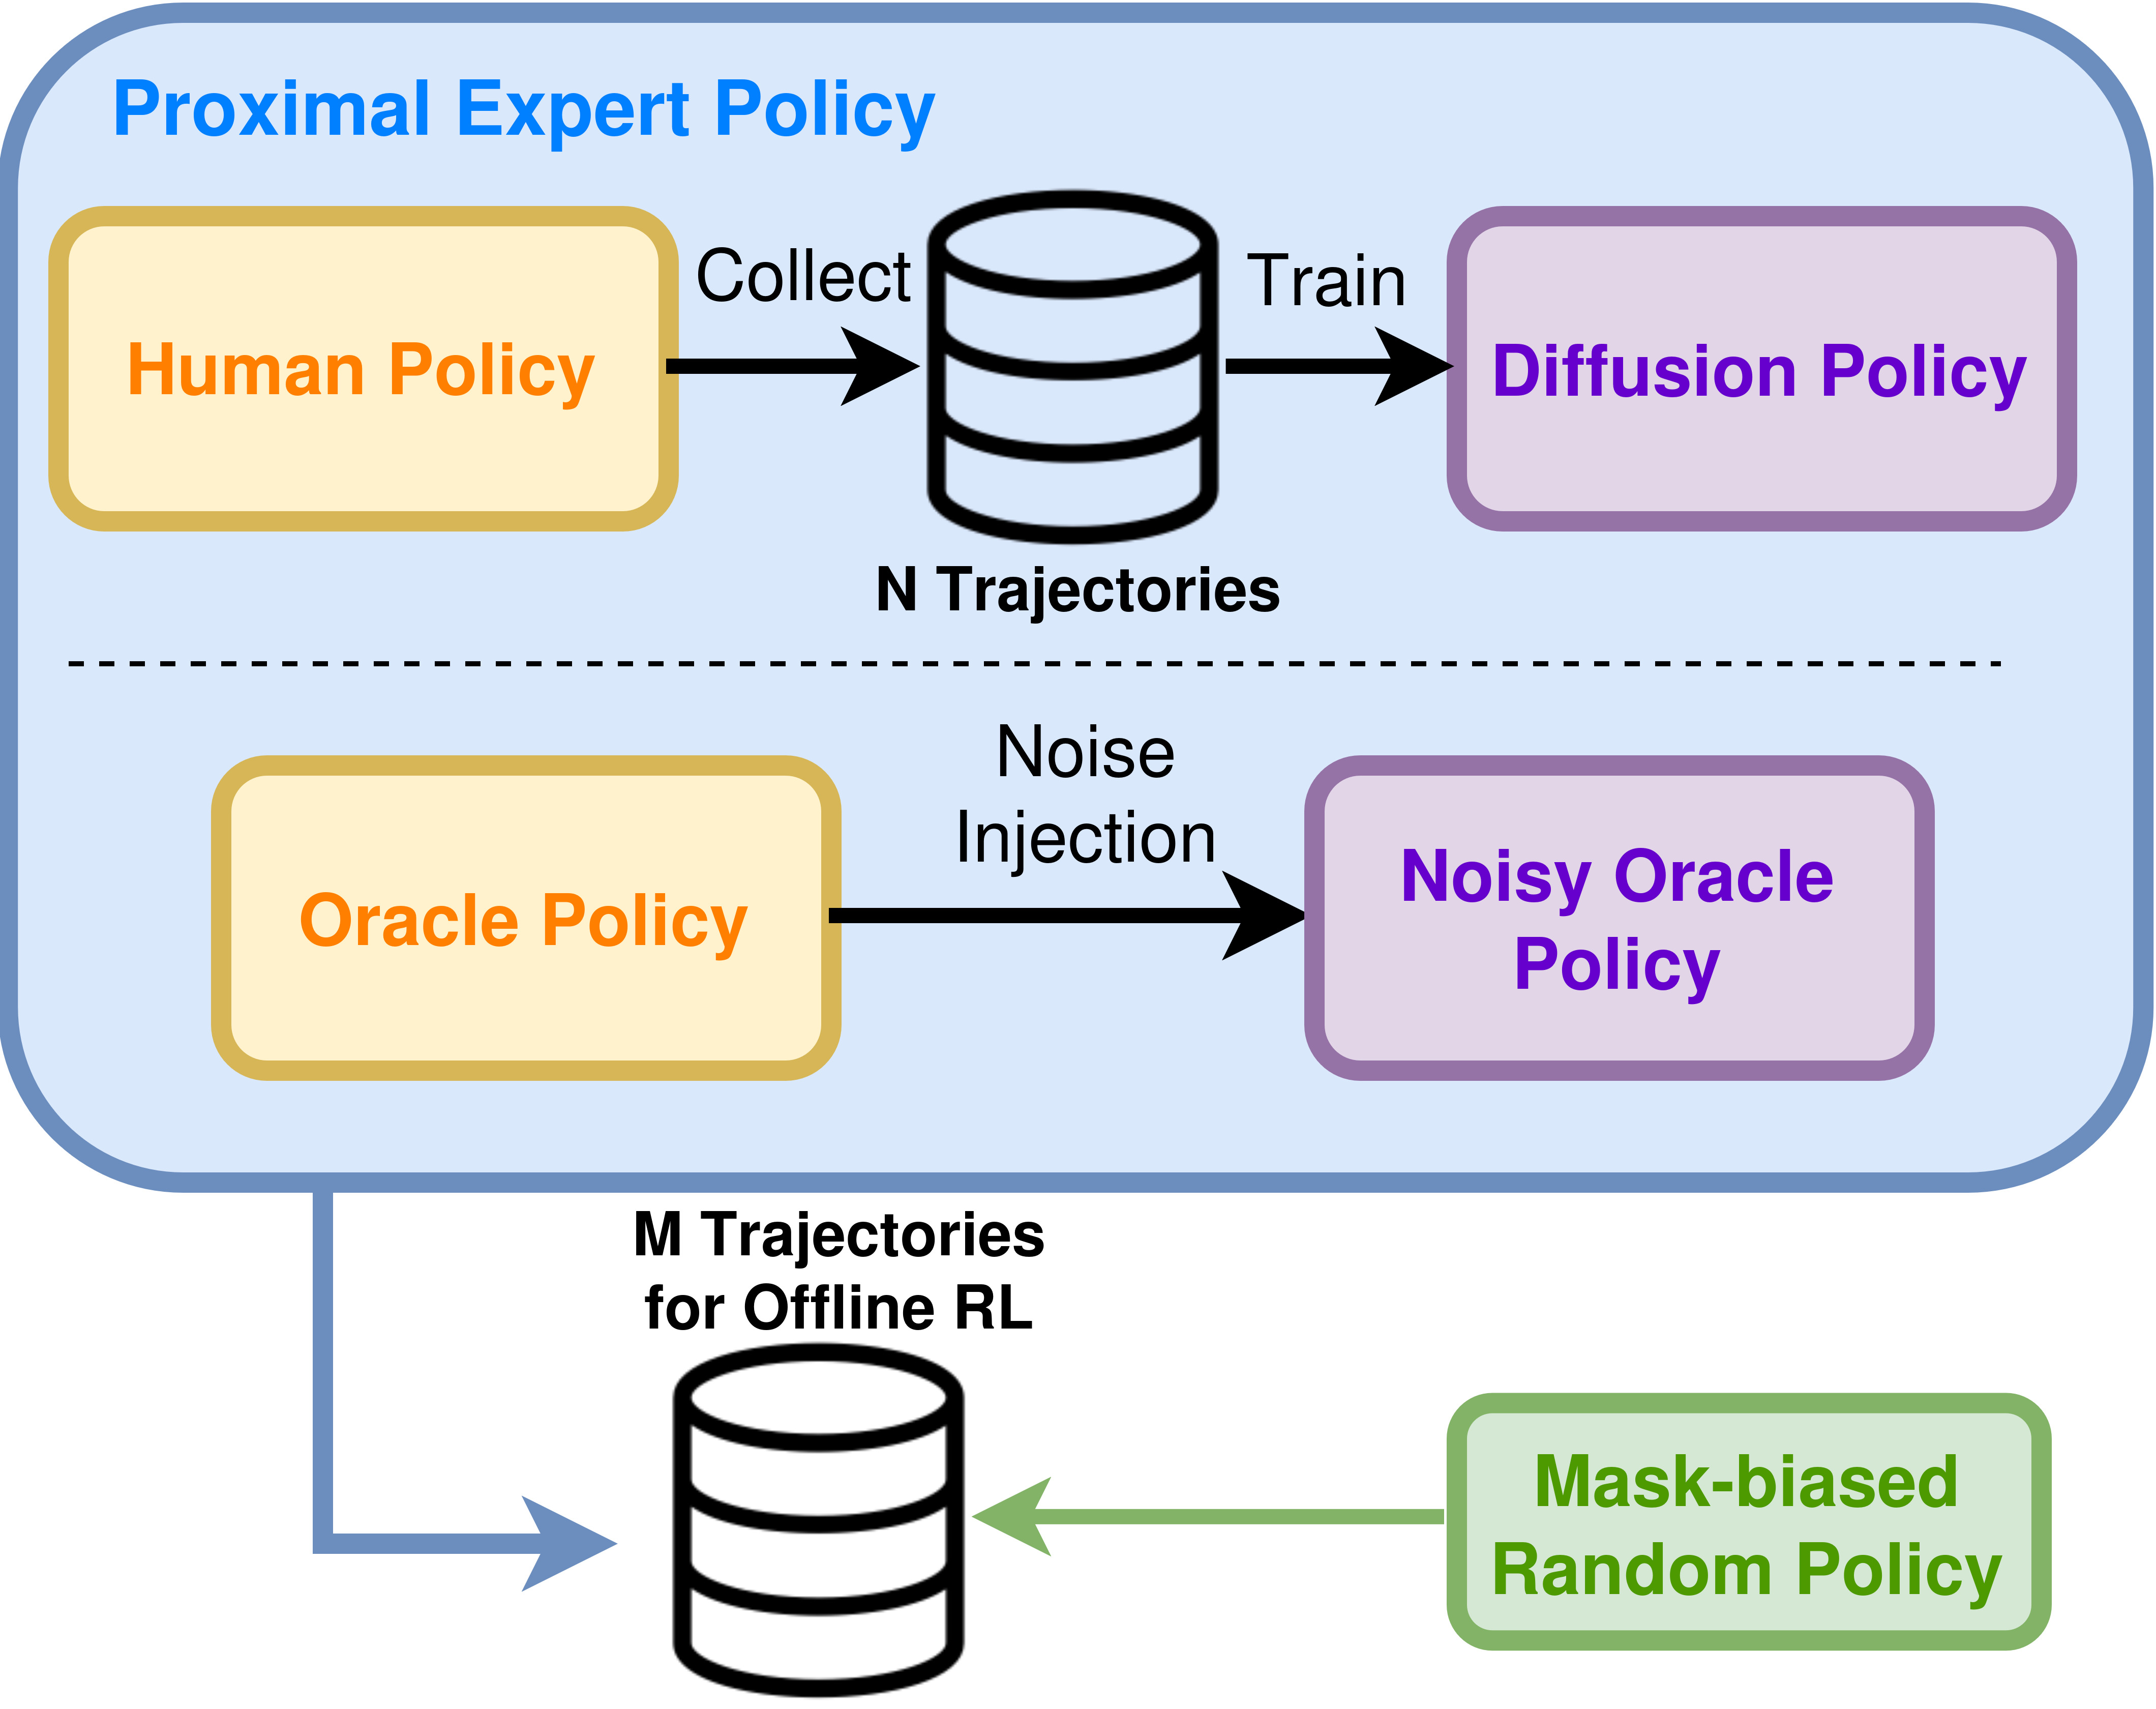
\includegraphics[width=\textwidth]{plots/lagarnet-data-collection.jpg}
%     \caption{Data Collection}
%         \label{fig:data-collection}
%     \end{subfigure}
%     % --- Main Overarching Caption ---
%     \caption{LaGarNet's Reward and Data Collection Procedure.}
%     \label{fig:lagarnet}
% \end{figure*}
\subsection{Proximal Expert and Random Policy Data Collection} \label{sec:data-collection}

Previous RSSM-based cloth flattening models \cite{kadi2024planet} rely on strong inductive biases stemming from a complex, specific blend of data collection policies. Engineering flattening oracles for complex garments such as T-shirts and trousers is extremely challenging, which defeats the simplicity advantage of imitation learning and hinders offline RL by preventing easy collection of trajectories around the successful region of the distribution. \text{LaGarNet} mitigates these biases with a proximal expert policy and a mask-biased random policy (Figure \ref{fig:data-collection}). 

We train a Diffusion Policy \cite{chi2023diffusionpolicy} (Appendix \ref{sec:diffusion}) on a few human demonstrations to replace the rigid oracle experts required by previous methods \cite{kadi2024planet}, because a true garment oracle is exceptionally difficult to develop and, as Figure~\ref{fig:longsleeve-flattening} shows, the Diffusion Policy induces numerous nearly successful flattening trajectories---its action diversity accounts for some manipulation noise, which we harness to diversify the data distribution around near-successful regions. 

To align exploration with the downstream object-masked MPC planner, which restricts pick positions to the cloth mask, we introduce a mask-biased random policy: rather than the fully random or corner-biased policies of prior work, it samples the pick pixel uniformly from the object mask and the place pixel uniformly from the image. Pairing the Diffusion Policy with this exploration at a 1:1 ratio curates a rich, targeted dataset and substantially reduces the inductive biases constraining earlier algorithms.
We train the proximal expert with the Diffusion Policy formulation adapted to the pick-and-place cloth domain by \textsc{DRAPER} \cite{kadi2025draper, chi2023diffusionpolicy}, and augment all policy inputs with appearance-level Gaussian noise, $SE(2)$ transformations of the current observation strictly coupled to the pixel action, and independent affine transformations of the goal observation. Appendices \ref{sec:diffusion} and \ref{sec:data-aug} give the formulation and exact augmentation parameters.

\section{Experiments} \label{sec:experiments}

Our experiments answer four research questions: how LaGarNet compares against state-of-the-art (SoTA) single-picker pick-and-place flattening baselines (Section \ref{sec:comp-sota}); what advantage the GC-RSSM model brings over a diffusion policy in this domain (Section \ref{sec:comp-diff}); how important each component of LaGarNet is (Section \ref{sec:abl}); and how LaGarNet performs in the real world (Section \ref{sec:real-exp}).

We evaluate our garment flattening policy with four standard metrics. \textbf{Normalised Coverage (NC)} is the ratio of the garment's current 2D projected area to its maximally flattened area, isolating the extent of unfolding and bounded to $[0,1]$. \textbf{Normalised Improvement (NI)} is the relative coverage increase from the initial configuration, $\frac{c_t - c_0}{c_{\text{max}} - c_0}$, with $c_t$, $c_0$ and $c_{\text{max}}$ the current, initial and maximally flattened coverage. \textbf{Maximum Intersection-over-Union (Max IoU)} is the highest IoU between the current garment mask and the target flattened mask over rotation and translation, evaluating precise spatial alignment and shape matching. \textbf{Success Rate (SR)} is the percentage of trials reaching a state with both $\text{NC} > 90\%$ and $\text{Max IoU} > 80\%$.

All metrics are cumulative over the horizon: at horizon $k$, NC, NI and Max IoU report the maximum reached within the first $k$ steps rather than the value at step $k$, and SR counts trials meeting the criteria at any step up to $k$. Unless stated otherwise we report a 20-step horizon. Simulated evaluation episodes nevertheless run to 30 steps: they are fully automated and the simulator is fast, so the extra steps are essentially free and reveal how each policy behaves once the easy gains are exhausted. Real-world trials stop at 20 steps, since a single physical step costs about 25\,s plus a manual reset (Section \ref{sec:real-exp}) and garments are generally flattened well within 20 steps. In both settings each garment's goal state (its maximally flattened configuration) is captured beforehand, serving as the ground-truth reference and as input to goal-conditioned policies: in simulation we use the states of Canberk et al.~\cite{canberk2023cloth}, whilst in the real world we first flatten the garment and then manually crumple it. We ignore the slight discrepancy caused by the relative position of garment and camera, as it does not noticeably affect training or evaluation.
\begin{table}[!t]
\centering
\caption{Simulation configurations. Garments in our longsleeve set are scaled down by 0.32 to obtain MEDOR's optimal performance.}
\label{tab:sim-config}
\begin{tabular}{@{}lcc@{}}
\toprule
\textbf{Parameter} & \textbf{Ours} & \textbf{MEDOR's} \\ \midrule
Garment Scale from Cloth3D & 0.8 & 0.32\\
Stiffness (Stretch, Bend, Shear) & (0.75, 0.02, 0.02) & (1.2, 0.6, 1.0) \\
Particle Radius (m) & 0.014 & 0.005 \\
Camera Height (m) & 2 & 0.65\\
FoV (degree) & 45 & 45\\
Mass (kg) & 1 (Total) & $3e^{-3}$ (Per Particle) \\
Dynamic/ Particle Frictions & 0.75 / 1.0&  1.0 / 1.2\\
Damping & 1 & 1 \\
\bottomrule
\end{tabular}
\end{table}

We train all models for 50,000 update steps and validate every 1,000 steps to save the best checkpoint. Simulation uses 200 training, 10 validation and 30 evaluation trials; training and validation trajectories are capped at 20 steps, whilst evaluation trials run the full 30. We compare checkpoints by a combined score summing average final NC and average Max IoU over the validation trials; if two checkpoints both exceed 1.90 (out of 2.0), we prefer the one completing the task in fewer steps, otherwise we take the highest combined score.

\subsection{Comparison of \text{LaGarNet} against Other Neural Controllers} \label{sec:comp-sota}

\begin{figure*}[t!]
\centering
\subfloat[Longsleeved T-shirt flattening against SoTA baselines.]{%
    
\includegraphics[width=0.56\linewidth]{plots/lagarnet_flattening_heatmap.png}%
    \label{fig:longsleeve-flattening}}\hfill
\subfloat[All-garment generalisation by action step 20.]{%
    
\includegraphics[width=0.40\linewidth]{plots/multi_arena_radar_2x2.png}%
    \label{fig:sim-lagarnet-results}}
\caption{Simulation results for single-arm pick-and-place (\text{PnP}) controllers. \textbf{(a)} Per-horizon longsleeve flattening: each metric reports the cumulative \emph{Max} (best value within the horizon) and the \emph{Last} (final-step) value at 5, 10, 20 and 30 steps; cell colour encodes the score in $[0,1]$. Only the single-arm PnP primitive of \text{ClothFunnels}~\cite{canberk2023cloth} is enabled; \text{Diffusion Policy}~\cite{kadi2025draper, chi2023diffusionpolicy} is trained on 200 human demonstrations, and \text{MEDOR}~\cite{huang2022mesh} is evaluated in its own simulation setup. All-Garment \text{LaGarNet} is comparable to MEDOR at a small fraction of its inference cost and competitive with human experts at intermediate horizons, although humans remain ahead at 30 steps. NC and Max IoU barely change between Max and Last, but the SR gap is large (76.7\% versus 13.3\% at 20 steps): LaGarNet reaches a success state without reliably remaining in it (Section \ref{sec:discussion}). \textbf{(b)} Performance on all four garment types by action step 20, where \text{LaGarNet} consistently outperforms all-garment \text{PlaNet-ClothPick} and task-specific \text{Diffusion Policy}.}
\label{fig:sim-results}
\end{figure*}



This section compares state-of-the-art (SoTA) single-arm pick-and-place (PnP) methods in simulation: the simulation setup (Section \ref{sec:simulation}), the baselines (Section \ref{sec:baseline}) and their primary and secondary performance (Section \ref{sec:sota-result}).

\subsubsection{Simulation Setup} \label{sec:simulation}

We develop \text{LaGarNet} in the garment simulation environment of Canberk et al.~\cite{canberk2023cloth}, built on SoftGym \cite{lin2020softgym} and the PyFlex physics engine \cite{li2018learning}, extended following the \text{DRAPER} real-world adaptation strategy \cite{kadi2025draper} to include the misgrasping and multi-layer grasping inherent to simple parallel grippers. We use the simulated longsleeved T-shirts, trousers, dresses and skirts that Canberk et al. selected from \text{Cloth3D} \cite{bertiche2020cloth3d} (Figure \ref{fig:sim-train-init}), scaled by 0.8 and rendered from a simulated top-down camera against a dark background; Table \ref{tab:sim-config} lists our simulation configuration. Canberk et al. split the generated initial garments into ``hard'' (more crumpled) and ``easy'' (more flattened) categories; we evaluate on 30 ``hard'' initial states placed within the gripper workspace, whose distribution is reported in Appendix \ref{sec:garment-dist}.


\subsubsection{Baseline Methods} \label{sec:baseline} 

We benchmark our model-based reinforcement learning (RL) method \textbf{LaGarNet} against past RSSM approaches like \textbf{PlaNet-ClothPick} \cite{kadi2024planet} and the off-the-shelf task-specific model-free method \textbf{ClothFunnels} \cite{canberk2023cloth} using its single-arm PnP primitives. We also compare against the state-of-the-art mesh-based planning method \textbf{MEDOR} \cite{huang2022mesh}  with its own simulation setup (see Table \ref{tab:sim-config})---we make sure our flattened garments are fully observable, looking similar to their own trial distribution. We also compare LaGarNet against the advanced deep behaviour cloning method \text{Diffusion Policy}, adapted for the PnP cloth-shaping domain \cite{chi2023diffusionpolicy, kadi2025draper}.  

All trained methods apart from \text{ClothFunnels} and \text{MEDOR} use the \text{DRAPER} vision processing strategy for sim-to-real transfer \cite{kadi2025draper}, which aligns real and synthetic RGB observations through real-world adaptation and domain randomisation in simulation and a refined grasping procedure. \text{Diffusion Policy} is trained on 200 human expert trajectories, whilst \text{LaGarNet} and \text{PlaNet-ClothPick} learn from 5,000 episodes (100,000 transitional steps) generated by our data-collection strategy; \text{PlaNet-ClothPick} shares LaGarNet's hyperparameters but uses a different reward function and no goal observations. The all-garment variants draw on all four garment types whilst keeping the task-specific data size. Human experiments use a PnP window interface operating directly on observation images in both settings.

\begin{table*}[t!]
    \centering
    \caption{Secondary comparison of computational requirements and data efficiency across garment flattening baselines. $\dagger$ marks values reported in the original paper; \text{ClothFunnels} uses 4 NVIDIA RTX 3090s. All our timing and parameter measurements use Ubuntu 24.04.4 LTS, an NVIDIA RTX 3090 Ti, an AMD Ryzen 9 5900X (12 cores, 2 threads per core) and 64\,GB RAM. Whilst the mesh-based method needs substantially less data-collection time, LaGarNet requires far fewer parameters and offers faster training and per-step inference.}
    \label{tab:efficiency-comparison}
    \resizebox{0.94\textwidth}{!}{%
    \begin{tabular}{lccccc}
    \toprule
    \textbf{Method} & \textbf{Data Size} & \textbf{Network Parameters (M)} & \textbf{$\sim$ Inference Time (s)} & \textbf{Data Collection Time (hrs)} & \textbf{Training Time (hrs)} \\
    \midrule
    ClothFunnels & 12,500 eps $\times$ 10 $P\&P$ $\dagger$ & 12.6 & 2 &  48 $\dagger$ &  48 $\dagger$ \\
    MEDOR & 5000 P\&P $\times$ 100 low-level steps $\dagger$ & 37.5 &  103 & 0.64 & 144 $\dagger$ \\
    % Task-Specific JA-TN & 200 eps $\times$ 20 $P\&P$  & 29.5 &  0.13 &  22 &  17 \\
    Task-Specific Diffusion Policy & 200 eps $\times$ 20 $P\&P$ & 83.7 &  1.5 &  22 & 35 \\
    All-Garment PlaNet-ClothPick & 5,000 eps $\times$ 20 $P\&P$ & 6.3 &  4 &  4 $\times$ 22 + max(75, 34) = 163 &  31 \\
    All-Garment LaGarNet & 5,000 eps $\times$ 20 $P\&P$ & 7.11 &  6 &  4 $\times$ 22 + max(75, 34) = 163 &  33 \\
    \bottomrule
    \end{tabular}
    }
\end{table*}

\subsubsection{Results} \label{sec:sota-result}

Figure \ref{fig:longsleeve-flattening} summarises flattening performance across all baselines. All-Garment LaGarNet is comparable to the state-of-the-art mesh-based planner MEDOR and competitive with the human baseline at intermediate horizons, although human experts retain the highest success rate at step 30, driven by their superior Max IoU. Trained on an equivalent volume of data, All-Garment LaGarNet consistently outperforms the Task-Specific LaGarNet trained on longsleeve data alone, showing that the architecture benefits from morphological diversity. Interestingly, given a long enough horizon (30 steps) the task-specific Diffusion Policy---despite only 200 human demonstrations and weak short-horizon behaviour---recovers to highly competitive results. Figure \ref{fig:sim-lagarnet-results} shows that the single-policy \text{LaGarNet} generalises, exceeding 95\% NC on every garment type at action step 20, though higher success rates on skirts and dresses indicate a bias towards simpler topologies.
Table \ref{tab:efficiency-comparison} reveals the accompanying trade-off. MEDOR attains a high Max IoU but needs a prohibitive $\sim$103\,s of inference per step and 37.5\,M parameters, whereas All-Garment \text{LaGarNet} needs only 7.11\,M parameters and roughly 6\,s per step, making it far more suitable for real-world deployment. \text{Diffusion Policy}, while fast, requires 83.7\,M parameters and still falls short of LaGarNet's success rate.
\begin{figure*}[t!]
    \centering
    
    % Subfigure A: Progression Plot
    \subfloat[\centering Validation Trials \label{fig:diffusion-human-val}]{
        
\includegraphics[width=0.26\textwidth]{plots/progression_nc_vs_iou.png}
    }\hfill
    % Subfigure B: Radar Chart
    \subfloat[\centering Evaluation Trials \label{fig:diffusion-human-eval}]{
        
\includegraphics[width=0.195\textwidth]{plots/metrics_radar.png}
    }\hfill
    % Subfigure C: The Table
    \subfloat[\centering Architectural Ablations \label{tab:comp-diff-lagarnet}]{
        \resizebox{0.42\textwidth}{!}{
            \begin{tabular}{lcccc}
            \toprule
            Method & SR & Max IoU & NC & NI \\
            \midrule
            GC-DP & 40.0 & 77.6 $\pm$ 6.6 & 89.7 $\pm$ 2.5 & 77.8 $\pm$ 4.8 \\
            GC-DP-Comp & 25.0 & 76.0 $\pm$ 6.6 & 87.2 $\pm$ 1.1 & 72.7 $\pm$ 2.7 \\
            LaGarNet-Comp & 5.0 & 69.1 $\pm$ 2.4 & 77.3 $\pm$ 5.0 & 49.4 $\pm$ 10.9 \\
            LaGarNet-RSSM & 52.5 & 82.0 $\pm$ 3.3 & 92.9 $\pm$ 0.9 & 84.6 $\pm$ 3.0 \\
            
            GC-RSSM-DP & 6.7 & 68.6 $\pm$ 3.4 & 77.4 $\pm$ 2.3 & 50.1 $\pm$ 5.0 \\
            LaGarNet-CNN-DP & 8.3 & 70.0 $\pm$ 3.6 & 78.2 $\pm$ 3.4 & 51.8 $\pm$ 6.5 \\

            \rowcolor{green!20} LaGarNet & 75.0 & 84.5 $\pm$ 3.0 & 95.4 $\pm$ 1.4 & 90.1 $\pm$ 3.4 \\
            \bottomrule
            \end{tabular}
        }
    }
    
    \caption{Diffusion Policy versus LaGarNet on the simulated longsleeve environment. \textbf{(a)} Validation performance over 50,000 training steps for task-specific Diffusion Policies trained with varying numbers of human demonstrations; bold lines are an exponential moving average (EMA, span = 15) of the success rate over the faint raw data. \textbf{(b)} Evaluation performance of these policies on the four primary metrics. \textbf{(c)} Architectural ablations by action step 20. All values are aggregated over 120 evaluation episodes (30 trials per garment type). The All-Garment LaGarNet trains stably and, on 5,000 episodes of mixed-quality transitions, substantially outperforms every Diffusion Policy variant trained on an equivalent volume of success-only trajectories.} 
    \label{fig:diff-vs-lagarnet-performance-combined}
\end{figure*}





\subsection{Diffusion Policy vs. LaGarNet}  \label{sec:comp-diff}


Using the setup of Section \ref{sec:simulation}, we ask whether LaGarNet's advantage over Diffusion Policy stems from explicit forward planning, from extended temporal context, or simply from data scale, examining how the number of human demonstrations affects a task-specific Diffusion Policy (Figures \ref{fig:diffusion-human-val} and \ref{fig:diffusion-human-eval}) alongside the ablated baselines below.


\subsubsection{Baselines} \label{sec:diff-baselines}

To isolate which architectural components drive LaGarNet's advantage, we design six baselines. (a) \textbf{GC-DP}: a Goal-Conditioned Diffusion Policy (Appendix \ref{sec:diffusion}) taking the concatenated current and goal RGB images, trained on 5,000 episodes of diffusion-induced, success-only data spanning all garment types. (b) \textbf{GC-DP-Comp}: GC-DP aligned to LaGarNet's hyperparameters---PlaNet's CNN encoder in place of ResNet-18, the two embeddings concatenated before the downstream networks, and the observation sequence length raised from 1 to 4. (c) \textbf{LaGarNet-Comp}: LaGarNet with its training sequence length cut from 50 to 4 for direct comparison. (d) \textbf{LaGarNet-RSSM}: LaGarNet using its full, unconditioned RSSM dynamics. (e) \textbf{GC-RSSM-DP}: GC-DP-Comp using LaGarNet's frozen pre-trained encoder and latent dynamics, with the noise predictor's conditioning dimension set to 360; each step wipes memory by zeroing the previous latent state and recovers the posterior by feeding a ``no-op'' action into the dynamics model. (f) \textbf{LaGarNet-CNN-DP}: GC-DP-Comp using only LaGarNet's frozen vision encoder, giving a 2048-dimensional embedding of the current and goal images. All policies use the hyperparameters of Table \ref{tab:all-hyperparameters}.c and identical data augmentation (Appendix \ref{sec:data-aug}).

\subsubsection{Results} \label{sec:diff-result}

LaGarNet substantially outperforms the diffusion baselines (Table \ref{tab:comp-diff-lagarnet}), reaching 72.5\% success against GC-DP's 40.0\% and leading on every metric at 96.1 $\pm$ 1.1\% NC and 91.3 $\pm$ 2.3\% NI---notable given that it trains on 5,000 episodes of mixed-quality transitions whereas GC-DP uses an equivalent volume of success-only data.

The ablations isolate why. Cutting the training sequence length to 4 (LaGarNet-Comp) collapses success to 5.0\%, so a long context horizon is essential for the long-horizon dynamics of deformable objects, and reverting to the unconditioned RSSM costs around 30\%, confirming the value of goal conditioning. Transplanting LaGarNet's pre-trained visual or latent representations into the diffusion framework yields only 8.3\% (LaGarNet-CNN-DP) and 6.7\% (GC-RSSM-DP): the diffusion baselines rest on a reactive end-to-end mapping from observations to action noise rather than a structured understanding of dynamics, so without the capacity to reason over future states they cannot exploit these representations. LaGarNet instead plans with its decoupled world model, a paradigm far better suited to long-horizon manipulation.
\subsection{Ablation Study on \text{LaGarNet}} \label{sec:abl}

\begin{figure*}[t!]
    \centering
    
    % --- LEFT COLUMN: Ablation Plots and Table ---
    \begin{minipage}[t]{0.5\textwidth}
        \vspace{0pt} % <-- TRICK: Forces top alignment of the minipage content
        \centering
        % Top Row (Left Column): Ablation Plots side-by-side
        \subfloat[\centering Latent Dynamic and Goal Ablation \label{fig:goal-ablation}]{
            
\includegraphics[width=0.42\linewidth]{plots/ablation_latent_bar.png}
        }
        \subfloat[\centering Reward Ablation \label{fig:reward-ablation}]{
            
\includegraphics[width=0.42\linewidth]{plots/ablation_reward_bar.png}
        }        
        
        \vspace{0.2cm} % Vertical spacing between plots and the table

        \subfloat[\centering Data Size Ablation \label{fig:datasize-ablation}]{
            
\includegraphics[width=0.42\linewidth]{plots/ablation_data_size_line.png}
        } 
        \subfloat[\centering Data Composition Ablation \label{fig:dataratio-ablation}]{
            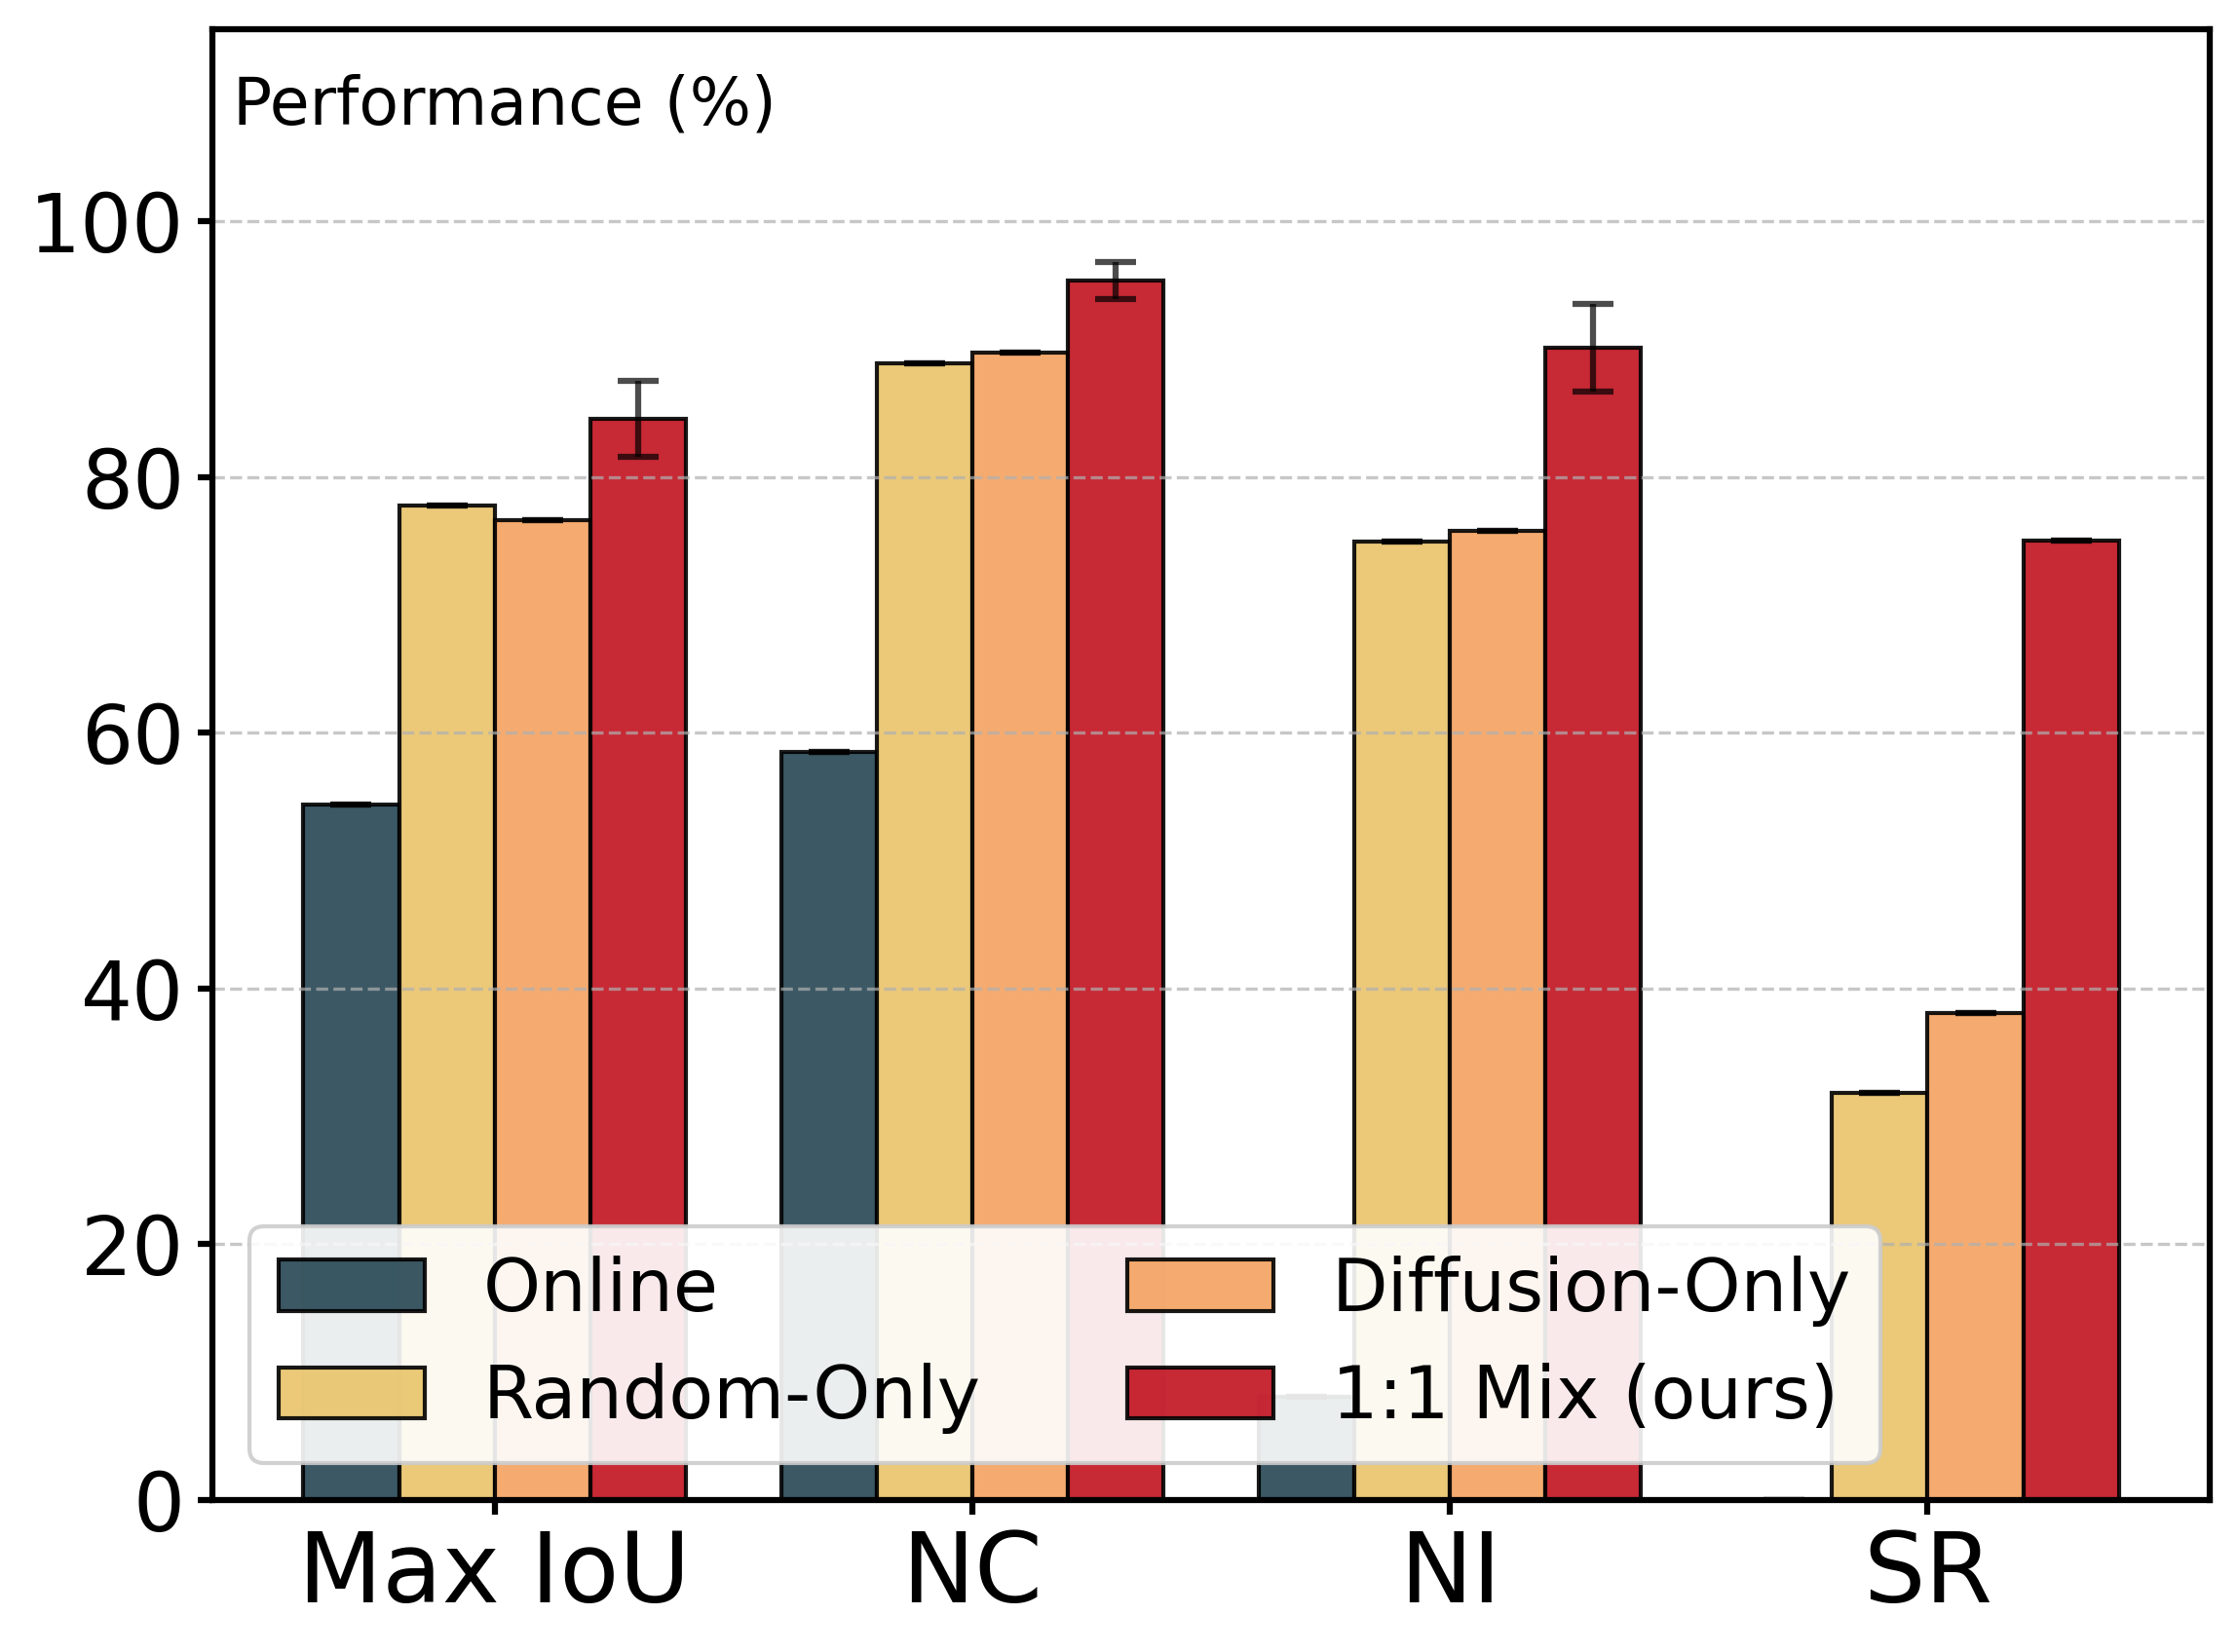
\includegraphics[width=0.42\linewidth]{plots/ablation_data_ratio_bar.png}
        } 
       
    \end{minipage}\hfill % <-- Spreading out the columns
    % --- RIGHT COLUMN: Reconstruction Image ---
    \begin{minipage}[t]{0.5\textwidth}
        \vspace{0pt} % <-- TRICK: Forces top alignment of the minipage content
        \centering
        \subfloat[\centering Observation reconstruction quality \label{fig:recon-quality}]{
            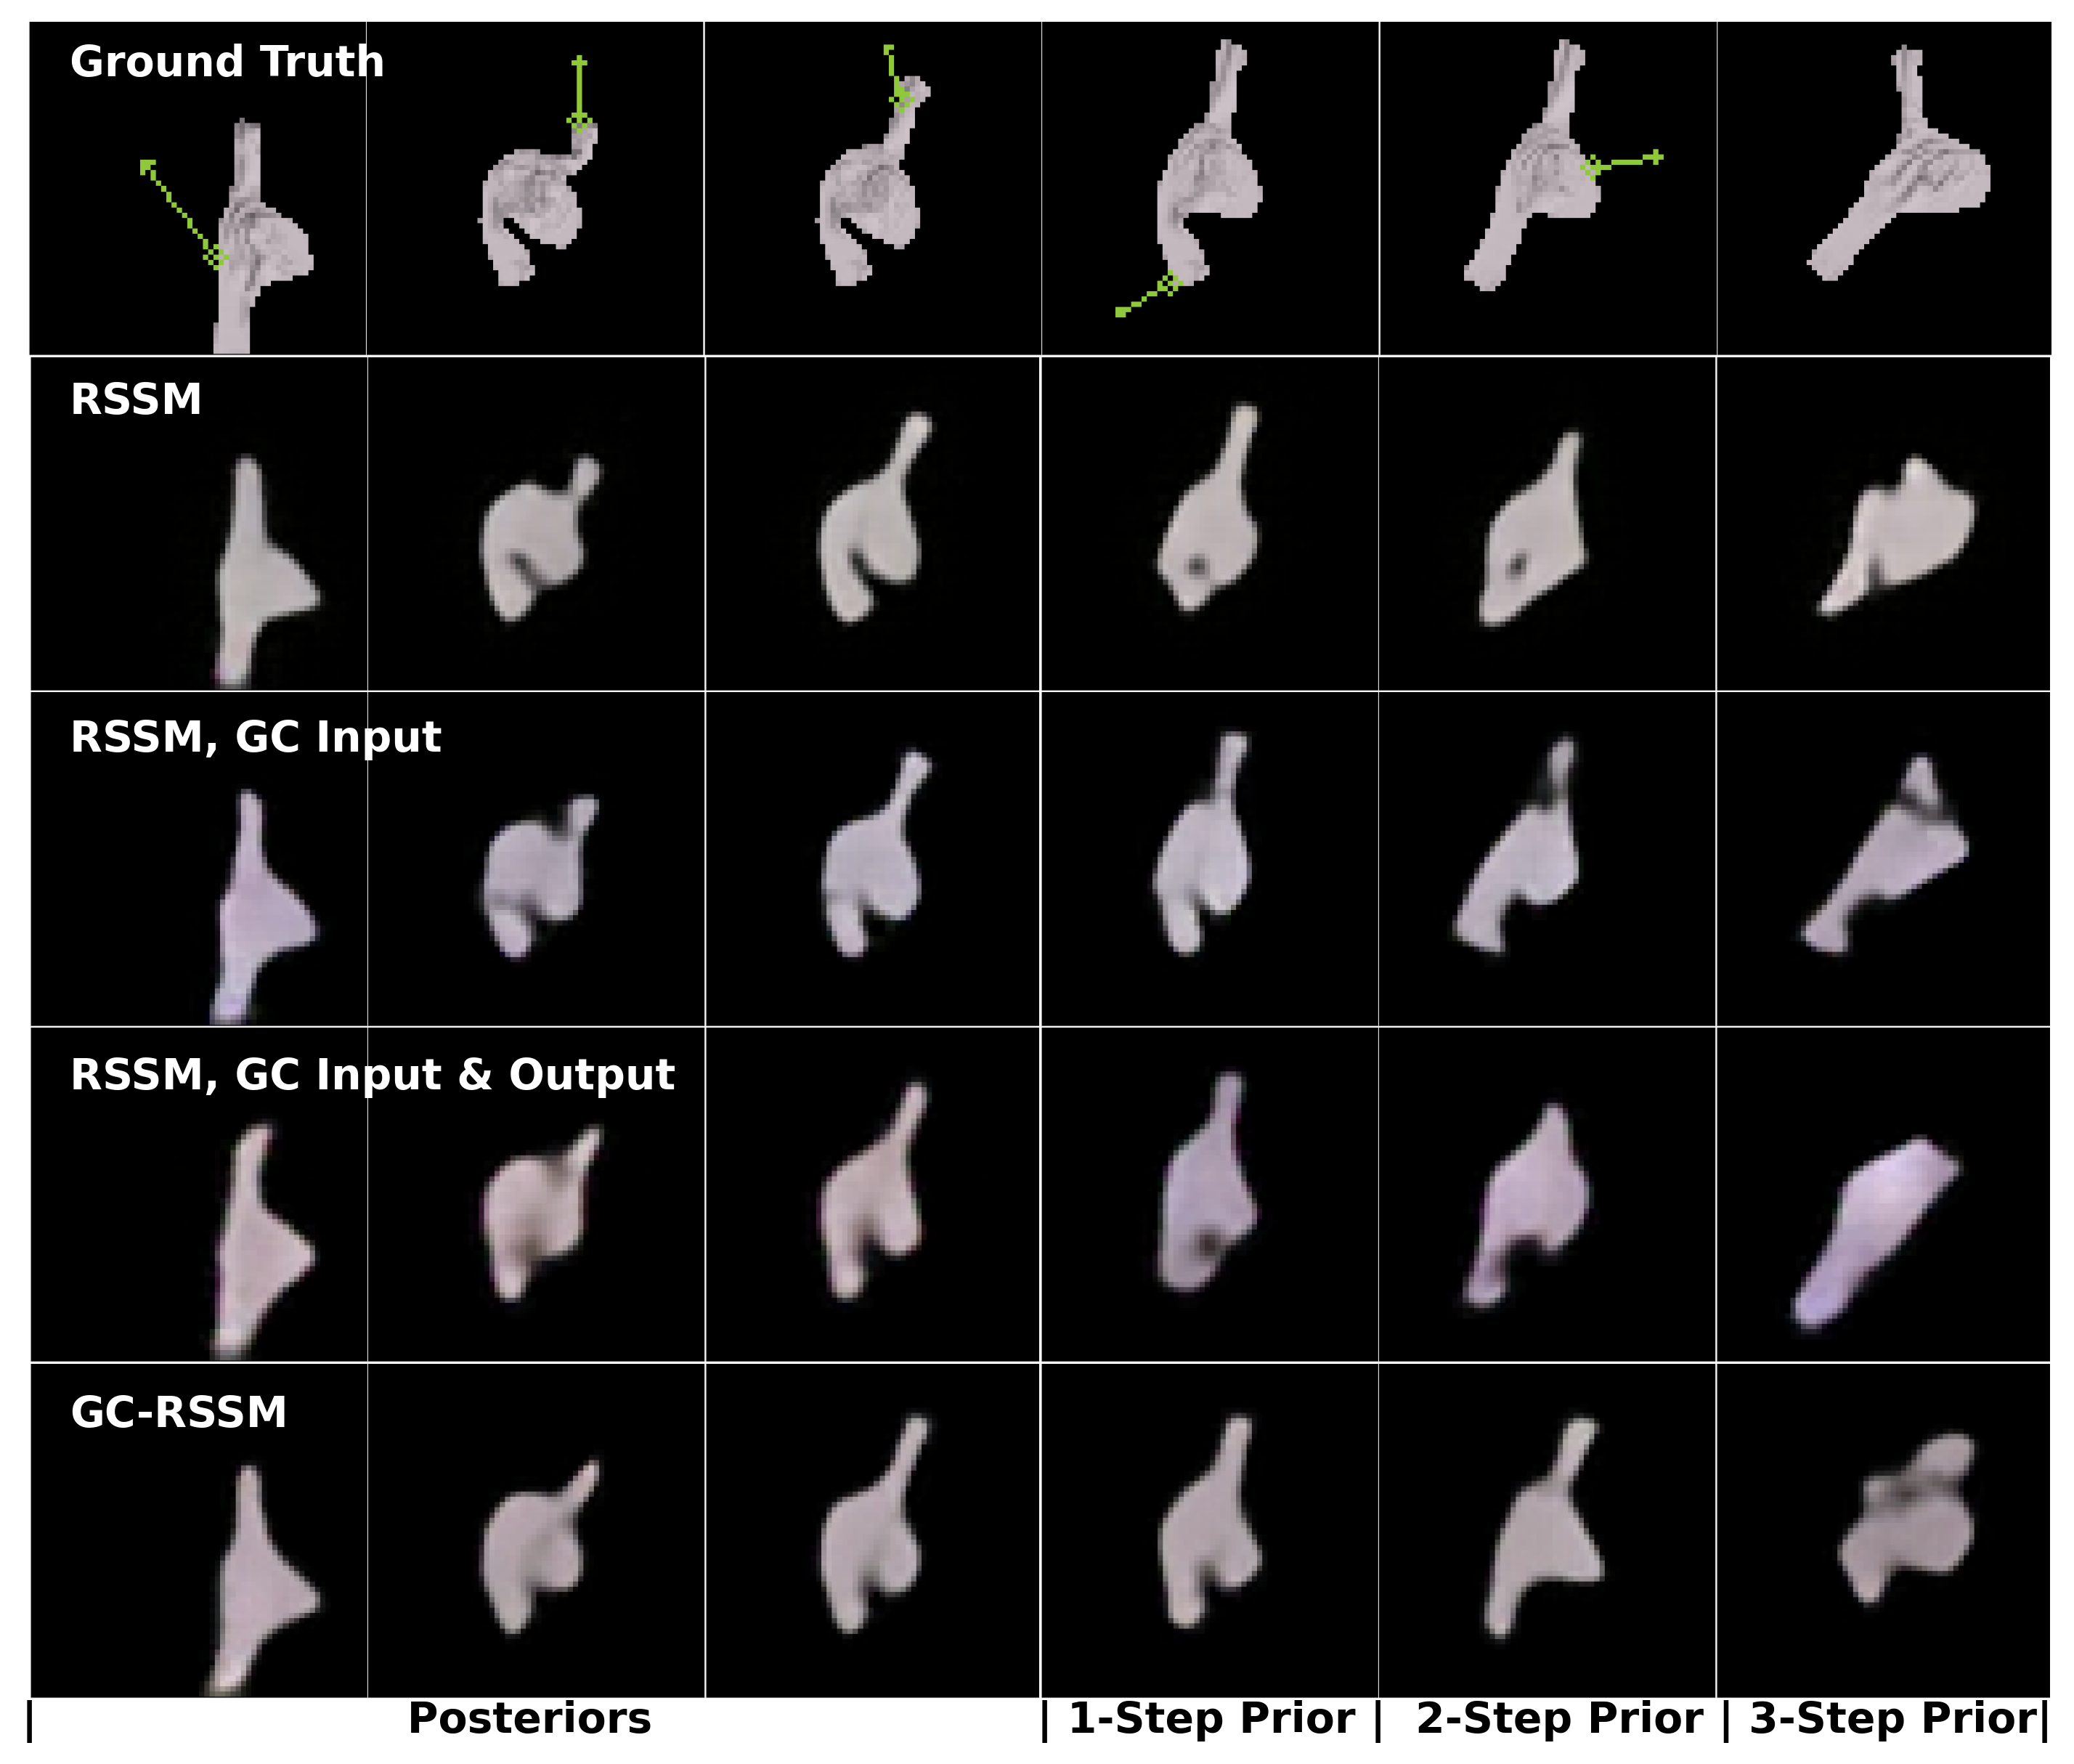
\includegraphics[width=0.88\linewidth]{plots/recon-all-garments.png}
        }
    \end{minipage}

    \vspace{0.2cm}

    % --- BOTTOM ROW: MPC planning-horizon ablation + reconstruction-quality table ---
    \subfloat[\centering MPC Planning Ablation $H$ \label{fig:horizon-ablation}]{%
        \begin{minipage}[b]{0.4\textwidth}
        \centering
        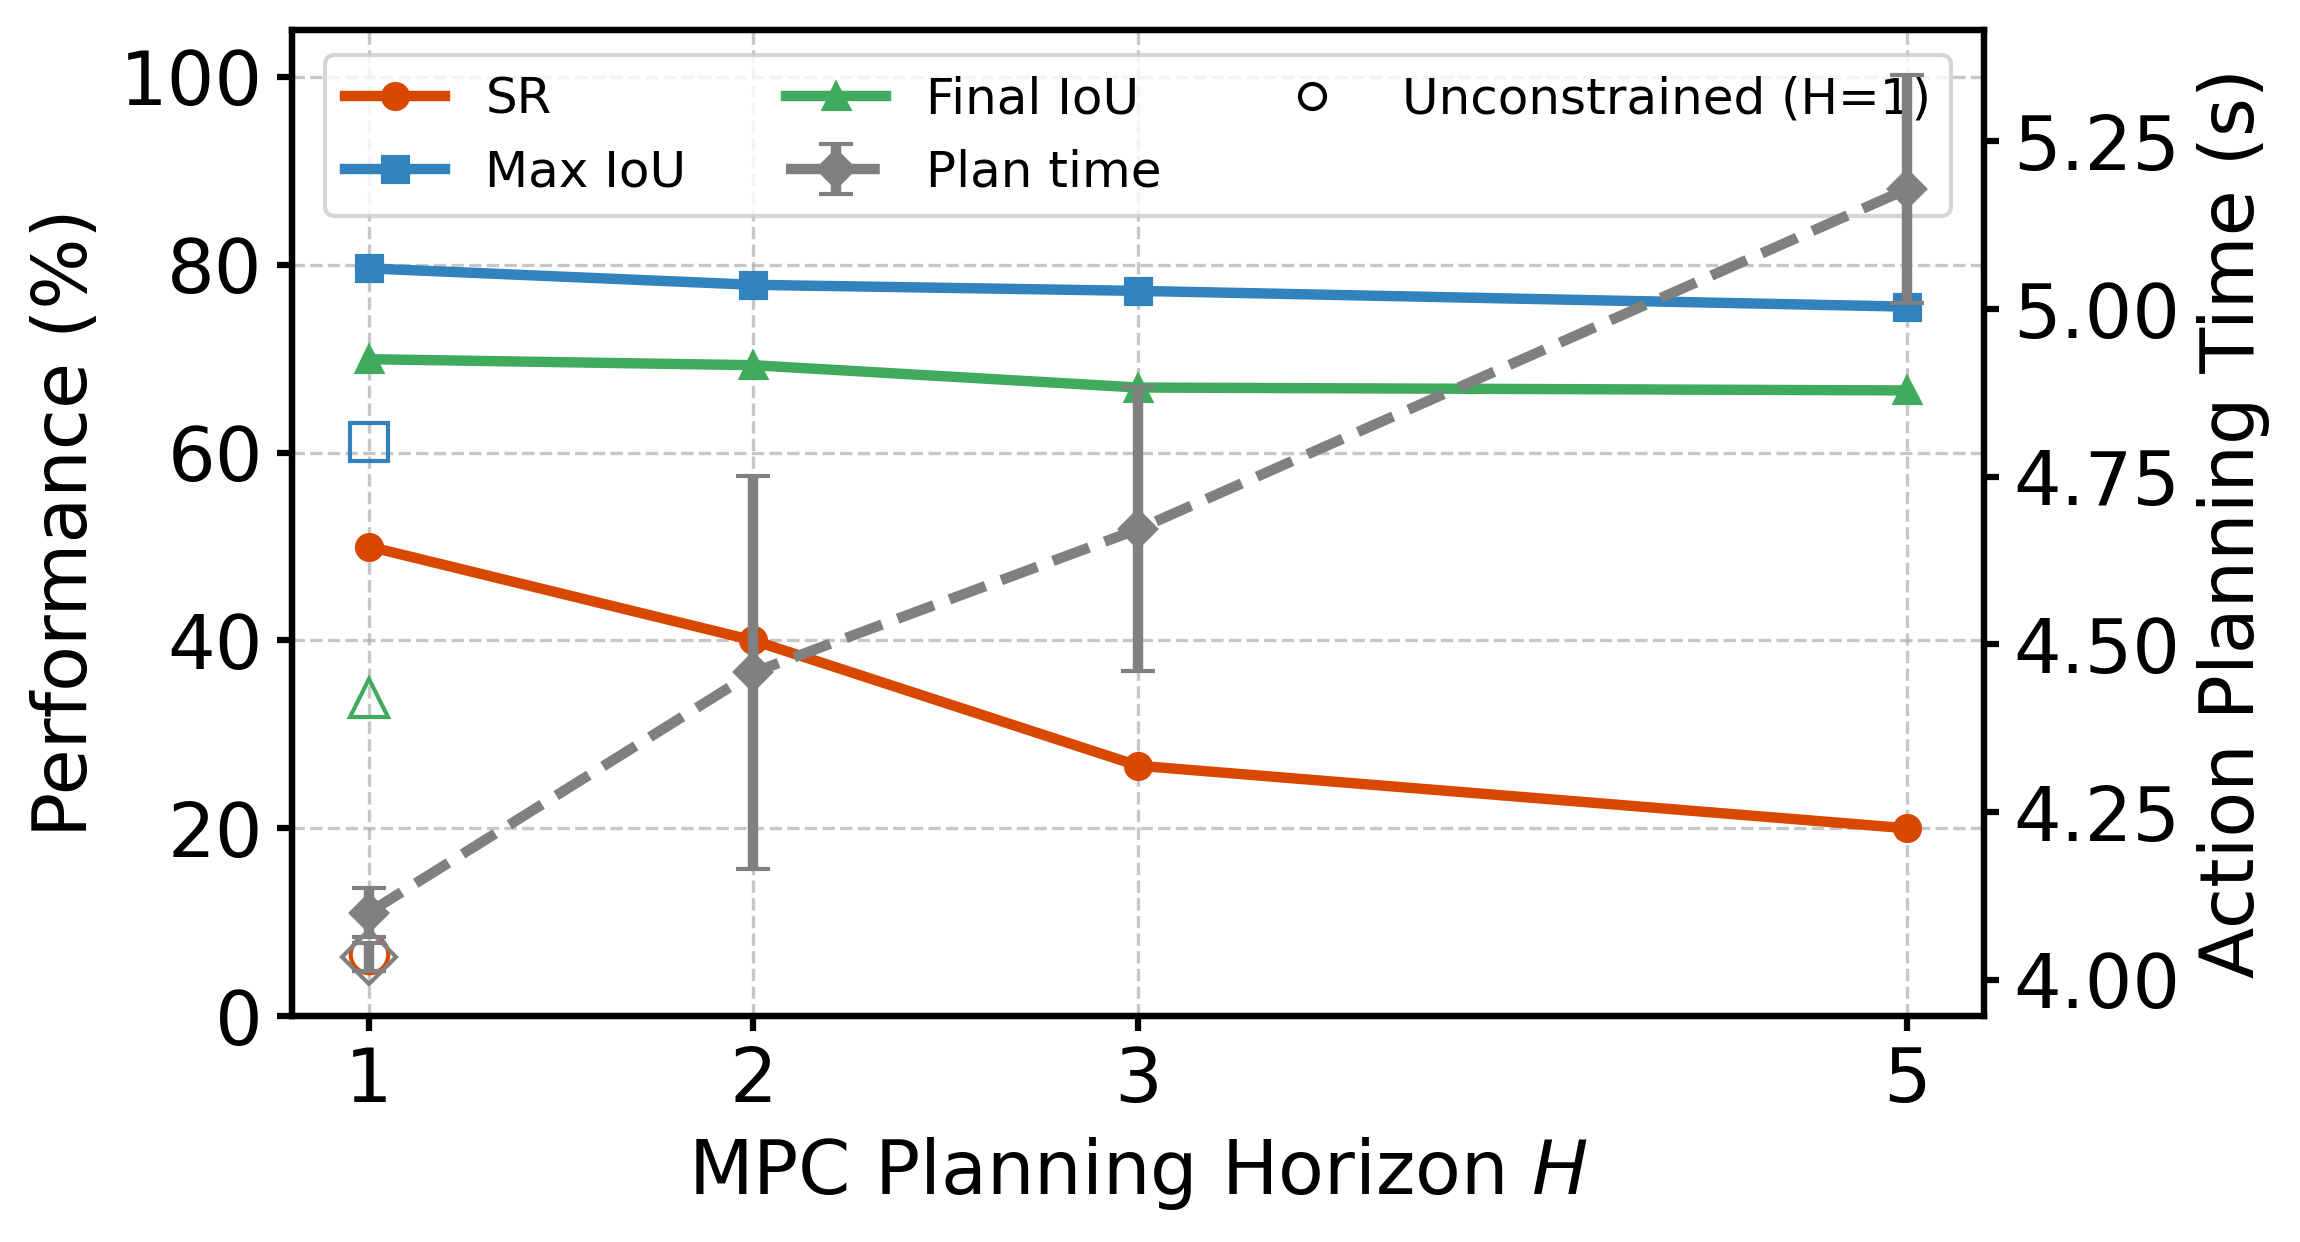
\includegraphics[width=\linewidth]{plots/ablation_mpc_horizon.png}
        \end{minipage}}
    \hfill
    \subfloat[\centering Reconstruction quality (MSE, SSIM) \label{tab:recon-quality}]{%
        \begin{minipage}[b]{0.53\textwidth}
        \centering
        \resizebox{\linewidth}{!}{%
        \setlength{\tabcolsep}{2pt}%
        \renewcommand{\arraystretch}{1.1}%
        \begin{tabular}{l|cc|cc|cc|cc}
         & \multicolumn{2}{c|}{Posterior} & \multicolumn{2}{c|}{Prior 1} & \multicolumn{2}{c|}{Prior 2} & \multicolumn{2}{c}{Prior 3} \\
        \hline
         Model, Metrics & MSE & SSIM   & MSE & SSIM   & MSE & SSIM   & MSE & SSIM  \\
        \hline
        RSSM & \textbf{0.26} & \textbf{94.09} &1.92 & 63.37 &2.60 & 62.00 &2.91 & 52.17\\
        RSSM, GC-I & 0.28 & 94.72 &1.87 & 65.58 &2.59 & 58.46 &2.80 & 56.05\\
        RSSM, GC-IO & 0.37 & 92.78 & \textbf{1.57} & \textbf{68.12} & \textbf{2.34}  & 62.10 &2.70 & 54.17\\
        GC-RSSM & 0.32 & 94.03 &1.67 & 67.72 &2.40 & \textbf{63.27} & \textbf{2.70} & \textbf{57.66}\\
        \bottomrule
        \end{tabular}}
        \end{minipage}}

    \caption{Comprehensive ablation study for LaGarNet in simulation environments. \textbf{(a, b, c, and d)} Ablation study using the all-garment LaGarNet models; all components of LaGarNet are essential for the success of this policy in garment flattening. \textbf{(e)} Observation reconstruction quality of models from Figure (a); each grid is a 64$\times$64 RGB image. The green arrows in the first row represent pick-and-place actions; our GC-RSSM model demonstrates a superior ability to track garment sleeves in prior steps compared to other RSSM variants. \textbf{(f)} Flattening performance (left axis) and mean per-action planning time (right axis) against the MPC planning horizon $H$; hollow markers report the unconstrained-CEM variant at $H=1$. \textbf{(g)} The reconstructions of (e) scored by Mean Squared Error (MSE) and Structural Similarity Index (SSIM) \cite{wang2004image}, both $\times$100 and averaged over 10 trials per garment; SSIM is informative here because it captures the local structure and contrast that blurring degrades. The models share all internal hyperparameters and differ only in structure and in their inputs and outputs; GC-RSSM reduces blurriness in the multi-step prior reconstructions.}
    \label{fig:ablation-and-recon-combined}
\end{figure*}
We ablate LaGarNet's components---latent dynamics, reward function, data size, dataset mixture ratio and planning horizon---in the simulation setup of Section \ref{sec:simulation}. All experiments use the default RGB-to-Mask variants except the latent dynamics ablations, which use RGB-to-RGB variants to inspect prediction quality (Figure \ref{fig:recon-quality}). Each model is evaluated on the 30 held-out hard initial states of all four garment arenas under the 20-step protocol and success criteria of Section \ref{sec:experiments}; the planning ablation isolates the longsleeve arena, the hardest of the four, and also logs per-action planning time.

\subsubsection{Ablation Baselines}


Alongside the \textbf{GC-RSSM} and \textbf{RSSM} models of Section \ref{sec:gc-rssm}, the latent dynamics ablation adds \textbf{RSSM-GC-I}, which takes the goal image concatenated with the current one but decodes only the current observation, and \textbf{RSSM-GC-IO}, which also predicts the goal image; together they separate goal-conditioning from GC-RSSM's structure. The reward ablation substitutes the alternatives of Section \ref{sec:reward-literature}: Learning2Unfold (\textbf{L2U}) \cite{gu2023learning}, ClothFunnels (\textbf{CF}) \cite{canberk2023cloth}, PlaNet-ClothPick (\textbf{PC}) \cite{kadi2024planet} and an approximation of SpeedFolding (\textbf{SFA}) \cite{avigal2022speedfolding}. The dataset ablations vary training-data volume and composition, including diffusion-only and random-only sets and an online LaGarNet that adds Gaussian noise to the MPC output following PlaNet's exploration strategy \cite{hafner2019learning}. The planning ablation sweeps $H \equiv T_f \in \{1,2,3,5\}$ and adds an \textbf{unconstrained} variant keeping $H = 1$ without the mask rejection of Appendix \ref{sec:planning}, separating the constrained action space from lookahead depth.
 
\subsubsection{Results}

LaGarNet's advantage stems from the combination of its GC-RSSM latent dynamics, its coverage-alignment reward and its data collection process. Figure \ref{fig:goal-ablation} shows the gain arises not only from goal-conditioning but from the structure of GC-RSSM: RSSM-GC-I performs similarly, whilst RSSM-GC-IO, which reconstructs both current and goal observations, performs much worse, likely because of the extra learning burden. Figures \ref{fig:recon-quality} and \ref{tab:recon-quality} confirm that GC-RSSM yields a superior prior latent state representation, which is crucial for planning and hence control. Figure \ref{fig:reward-ablation} shows the coverage-alignment reward is essential, with only the SFA reward approaching it, whilst Figures \ref{fig:datasize-ablation} and \ref{fig:dataratio-ablation} show performance plateauing beyond 1,000 episodes and confirm that the data collection procedure is critical.

Figure \ref{fig:horizon-ablation} shows the greedy one-step planner is strongest: success falls monotonically from 50.0\% at $H=1$ to 40.0\%, 26.7\% and 20.0\% at $H=2,3,5$, whilst mean planning time rises from 4.10\,s to 5.18\,s. A single primitive causes one large deformation, so prediction error compounds along multi-step rollouts and lookahead costs more than it buys, unlike in continuous control \cite{hafner2019learning}. The action constraint matters far more: dropping mask rejection at $H=1$ collapses success to 6.7\% and final IoU to 33.8, as most samples then miss the garment. This justifies $T_f=1$.


\subsection{Transfer Ability of LaGarNet to Real-World Settings} \label{sec:real-exp}

\begin{table*}[t!]
\caption{Real-world garment flattening performance of different pick-and-place controllers. The mesh-based planning method VCD \cite{lin2022learning} reports reaching \colorbox{yellow!25}{79.2 $\pm$ 9.4 \% NI} and \colorbox{yellow!25}{77.3 $\pm$ 14.1 \% NC} for real T-shirt flattening within 20 steps; its improved successor, MEDOR, reports achieving around \colorbox{gray!25}{64\% NI} flattening for real trousers and \colorbox{gray!25}{46.8\% NI} for real dresses within 10 steps. LaGarNet shows substantial performance improvements across all garments compared to PlaNet-ClothPick, though it still falls short of human-level performance.}
\label{tab:real-worldflattening}
\centering
\resizebox{0.96\textwidth}{!}{%
\renewcommand{\arraystretch}{1.1} 
\setlength{\tabcolsep}{2pt}
% Updated column structure: 13 total columns instead of 16
\begin{tabular}{c|cccc|cccc||cccc}
% Updated multicolumn spans from 5 to 4
Method & \multicolumn{4}{c|}{All-Garment PlaNet-ClothPick \cite{kadi2024planet}}  & \multicolumn{4}{c||}{All-Garment LaGarNet} & \multicolumn{4}{c}{Human Policy} \\
\cline{1-13} % Updated to reflect 13 columns
% Updated headers to a single SR
10 Steps & NC $\uparrow$  & NI $\uparrow$ & Max IoU $\uparrow$    & SR  $\uparrow$ 
& NC $\uparrow$  & NI $\uparrow$ & Max IoU $\uparrow$     & SR  $\uparrow$ 
& NC $\uparrow$  & NI $\uparrow$ & Max IoU $\uparrow$    & SR  $\uparrow$ \\
\hline
Longsleeve & 67.1 $\pm$ 12.7 & 30.4 $\pm$ 20.9 & 63.2 $\pm$ 10.3 & 0/10 & 73.4 $\pm$ 8.2 & 52.0 $\pm$ 16.2 & 66.3 $\pm$ 7.0 & 1/10 & 89.1 $\pm$ 7.8 & 81.0 $\pm$ 13.8 & 78.5 $\pm$ 6.3 & 4/10 \\
Trousers & 60.6 $\pm$ 16.4 & 24.1 $\pm$ 21.9 & 57.9 $\pm$ 14.9 & 1/10 & 78.7 $\pm$ 10.8 & \cellcolor{gray!25} 57.2 $\pm$ 17.0 & 70.1 $\pm$ 9.2 & 3/10 & 96.4 $\pm$ 5.5 & 93.0 $\pm$ 10.9 & 85.7 $\pm$ 7.7 & 9/10 \\
Dress & 71.9 $\pm$ 19.5 & 74.6 $\pm$ 28.8 & 69.5 $\pm$ 16.4 & 3/10 & 99.0 $\pm$ 2.2 & \cellcolor{gray!25} 97.6 $\pm$ 6.0 & 88.6 $\pm$ 2.7 & 10/10 & 94.7 $\pm$ 12.0 & 91.3 $\pm$ 19.8 & 85.3 $\pm$ 8.5 & 9/10 \\
Skirt & 76.1 $\pm$ 17.1 & 44.0 $\pm$ 26.1 & 74.1 $\pm$ 15.5 & 4/10 & 87.7 $\pm$ 11.8 & 75.7 $\pm$ 22.2 & 83.9 $\pm$ 9.5 & 8/10 & 95.4 $\pm$ 6.8 & 85.9 $\pm$ 24.7 & 91.0 $\pm$ 5.1 & 8/10 \\
\hline
Real Total & 69.0 $\pm$ 17.6 & 43.3 $\pm$ 31.4 & 66.2 $\pm$ 15.7 & 8/40 & 84.7 $\pm$ 13.3 & 70.6 $\pm$ 24.3 & 77.2 $\pm$ 12.0 & 22/40 & 93.9 $\pm$ 8.8 & 87.8 $\pm$ 18.7 & 85.1 $\pm$ 8.3 & 30/40 \\
\hline
\hline
20 Steps 
% Updated headers to a single SR
& NC $\uparrow$  & NI $\uparrow$ & Max IoU $\uparrow$    & SR  $\uparrow$ 
& NC $\uparrow$  & NI $\uparrow$ & Max IoU $\uparrow$     & SR  $\uparrow$ 
& NC $\uparrow$  & NI $\uparrow$ & Max IoU $\uparrow$    & SR  $\uparrow$ \\
\hline
Longsleeve & 69.2 $\pm$ 13.2 & 34.6 $\pm$ 22.1 & 64.5 $\pm$ 10.3 & 0/10 & \cellcolor{yellow!25} 84.5 $\pm$ 7.9 & \cellcolor{yellow!25} 71.1 $\pm$ 17.0 & 74.1 $\pm$ 6.8 & 4/10 & 96.8 $\pm$ 7.6 & 94.2 $\pm$ 13.9 & 87.6 $\pm$ 5.8 & 9/10 \\
Trousers & 60.6 $\pm$ 16.4 & 24.1 $\pm$ 21.9 & 57.9 $\pm$ 14.9 & 1/10 & 80.2 $\pm$ 10.3 & 60.1 $\pm$ 16.9 & 70.5 $\pm$ 9.0 & 3/10 & 100.0 $\pm$ 0.0 & 100.0 $\pm$ 0.0 & 93.6 $\pm$ 0.7 & 10/10 \\
Dress & 75.8 $\pm$ 19.5 & 90.6 $\pm$ 17.7 & 72.5 $\pm$ 16.2 & 3/10 & 100.0 $\pm$ 0.0 & 100.0 $\pm$ 0.0 & 89.5 $\pm$ 1.9 & 10/10 & 100.0 $\pm$ 0.0 & 100.0 $\pm$ 0.0 & 89.2 $\pm$ 1.7 & 10/10 \\
Skirt & 80.4 $\pm$ 17.1 & 54.0 $\pm$ 31.7 & 77.4 $\pm$ 14.7 & 5/10 & 96.5 $\pm$ 3.2 & 91.4 $\pm$ 9.8 & 90.4 $\pm$ 2.3 & 10/10 & 97.4 $\pm$ 5.7 & 90.3 $\pm$ 24.2 & 92.6 $\pm$ 4.2 & 9/10 \\
\hline
Real Total & 71.5 $\pm$ 18.3 & 50.8 $\pm$ 34.9 & 68.1 $\pm$ 16.0 & 9/40 & 90.3 $\pm$ 10.6 & 80.7 $\pm$ 20.4 & 81.1 $\pm$ 10.7 & 27/40 & 98.6 $\pm$ 5.0 & 96.1 $\pm$ 14.5 & 90.7 $\pm$ 4.4 & 38/40 \\
\bottomrule
\end{tabular}
}
\end{table*}

Our zero-shot real-world study assesses the simulation-trained LaGarNet and PlaNet-ClothPick policies of Section \ref{sec:sota-result} across all four garment types, whose colour, size and material properties are shown in Figure \ref{fig:real-garments}. MEDOR is excluded because of its prohibitive execution time and the difficulty of tuning its camera setup, and Diffusion Policy because adapting its action inference to our workspace constraints is non-trivial. To stress-test the system we additionally evaluate a soft longsleeved dress with high internal friction, an out-of-distribution ``unseen'' garment whose topology is absent from the simulated training set. 

We employ a UR5e arm with an OnRobot RG2 parallel gripper, observed by a RealSense D435i camera mounted in front of the robot above a dark table surface; Appendix \ref{sec:real-world-setup} details the setup, hand-eye calibration, segmentation, grasping and workspace transfer heuristic. All physical experiments run on a laptop with Ubuntu 20.04 LTS, an Intel Core i7-12700H, 16\,GB RAM and an NVIDIA RTX 3080 (16\,GB VRAM). Given the sim-to-real gap we relax the success criteria to NC $\geq$ 85 and Max IoU $\geq$ 75, and cap each real-world trial at 20 rather than 30 steps: a perception-action cycle takes about 25\,s (Table \ref{tab:timing_metrics}) plus manual garment resets, so extending every trial to 30 steps would add hours of robot time whilst most trials plateau before step 20 (Table \ref{tab:real-worldflattening}). We also analyse computational time consumption and provide a step-wise and trajectory-level failure analysis.

\begin{figure*}[t!]
    \centering
    % --- LEFT SIDE: The Image (Subfigure a) ---
    \begin{subfigure}[b]{0.38\textwidth}
        \centering
        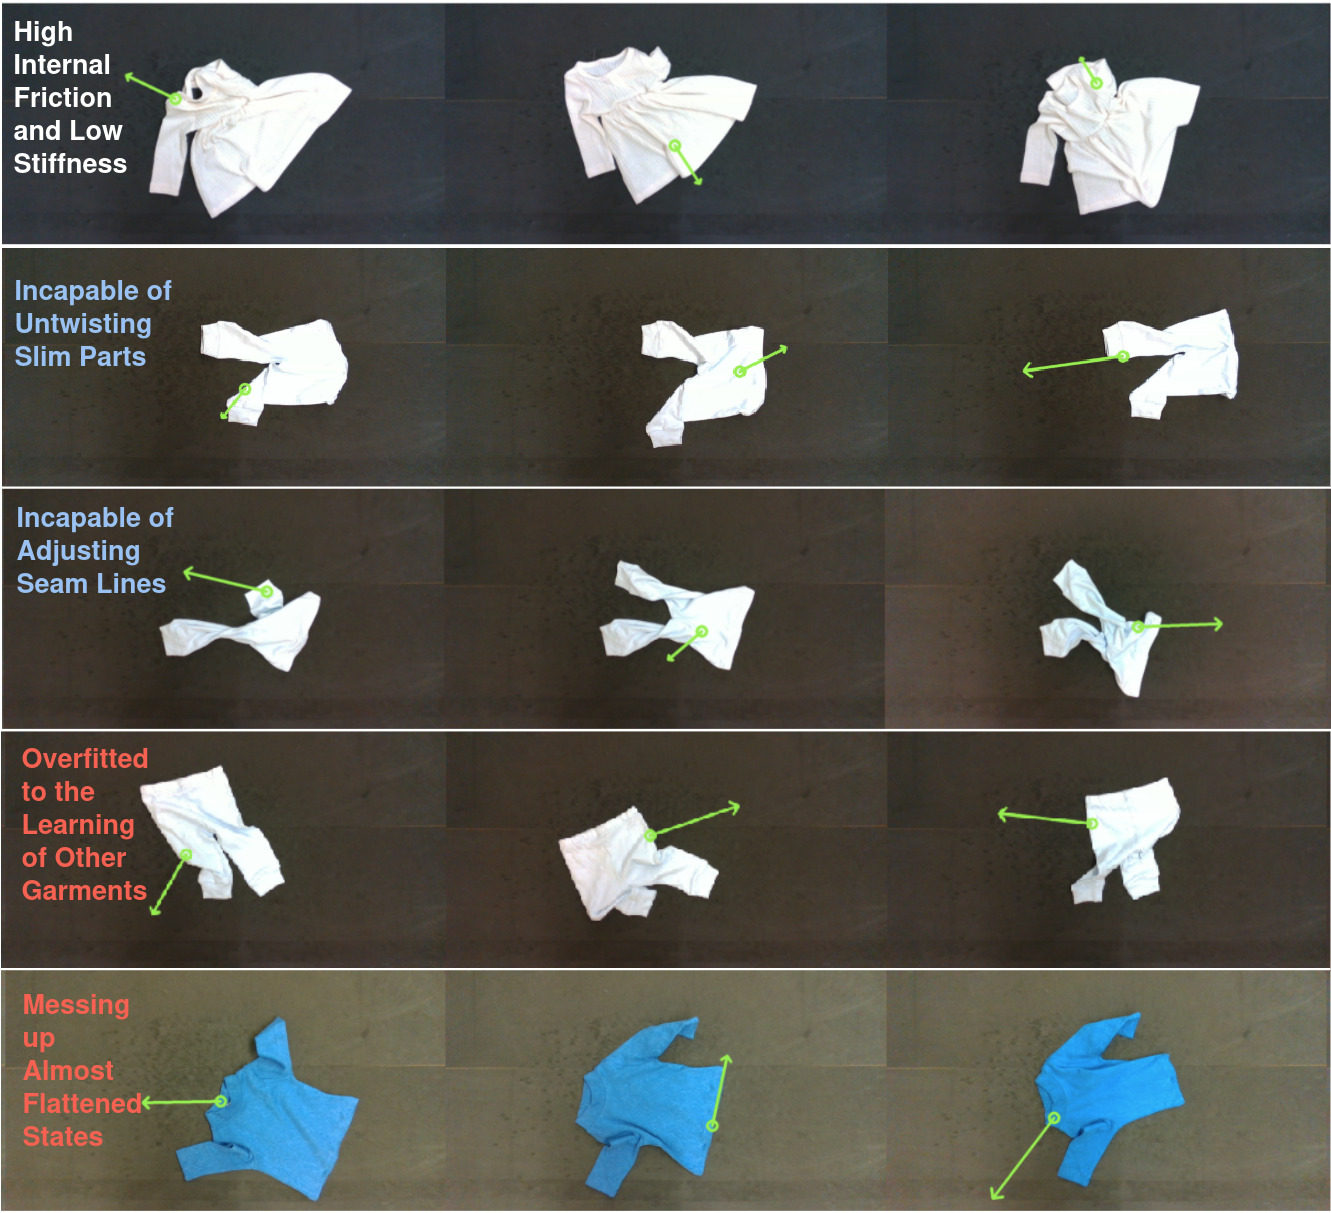
\includegraphics[width=\linewidth]{plots/lagarnet-failure.jpg}
        \caption{Visual failure cases of LaGarNet.}
        \label{fig:failure-visuals}
    \end{subfigure}
    \hfill % Flexible space between left and right sides
    % --- RIGHT SIDE: Stacked Tables ---
    \begin{minipage}[b]{0.58\textwidth}

        % --- TOP RIGHT: Failure Modes (Subtable b) ---
        \begin{subtable}[b]{\linewidth}
            \centering
            \footnotesize
            \begin{tabular}{@{}llc@{}}
            \toprule
            \textbf{Failure Category} & \textbf{Specific Mode} & \textbf{Rate} \\ \midrule
            \multirow{3}{*}{\textbf{Trajectory}} 
            & Fold Underneath & 3/40 \\
            & Fold On the Top & 2/40 \\
            & Cannot untwist & 5/40 \\
            & Cannot stabilise on success state & 4/40 \\ \midrule
            \multirow{4}{*}{\textbf{Step-wise}} 
            & Segmentation failure & 1/800 \\
            & Misgrasping failure & 3/800 \\
            & Messing-near-success state & 168/298 \\
            & As-if-manipulating-other-object & 28/800 \\ \bottomrule
            \end{tabular}
            \caption{Trajectory and step-wise failure rates.}
            \label{tab:failure-rates}
        \end{subtable}
        
        \vspace{0.1in} % Vertical space between the top and bottom rows
        
        % --- BOTTOM ROW: Two Side-by-Side Tables ---
        
        % Bottom Left: Timing Metrics (Subtable c)
        \begin{subtable}[b]{0.55\linewidth}
            \centering
            \footnotesize
            \begin{tabular}{@{}lc@{}}
\toprule
\textbf{System Phase} & \textbf{Time (s)} \\ \midrule
Perception & 8.19 \\
Action Inference & 7.05 \\
Action Conversion & 0.03 \\
Robot Execution & 9.20 \\
\bottomrule
\end{tabular}
            \caption{Average Time Consumption}
            \label{tab:timing_metrics}
        \end{subtable}
        %\hfill % Pushes the two bottom tables to the edges
        % Bottom Right: Unseen Dress Metrics (Subtable d)
        \begin{subtable}[b]{0.42\linewidth}
            \centering
            \footnotesize
            \begin{tabular}{@{}lc@{}}
\toprule
\textbf{Metric} & \textbf{Score} \\ \midrule
NC & 77.2 $\pm$ 6.5 \\
NI & 42.1 $\pm$ 22.6 \\
Max IoU & 66.4 $\pm$ 3.2 \\
SR & 0/10 \\
\bottomrule
\end{tabular}
            \caption{Unseen long-sleeve dress.}
            \label{tab:unseen-dress}
        \end{subtable}
        
    \end{minipage}
    
    \vspace{0.1in} % Space between the sub-elements and the main caption
    
    % --- GENERAL CAPTION FOR THE ENTIRE FIGURE* ---
    \caption{Analysis of LaGarNet's real-world performance. \textbf{(a)} Failure cases; text colour indicates the source of failure: white for mechanical limitations, blue for assumption oversights, red for the learning process. \textbf{(b)} Failure-mode frequencies. A step-wise failure does not necessarily cause a trajectory failure; a trajectory succeeds if it reaches the success state within 20 steps. ``Messing-near-success state'' counts how often performance drops in the step immediately after a ``near-success'' step (NC $\geq$ 0.8 and IoU $\geq$ 0.7). \textbf{(c)} Timing breakdown across the perception-action cycle. \textbf{(d)} Zero-shot generalisation to an unseen longsleeved dress with soft material properties and high internal friction.}
    \label{fig:real_world_analysis}
\end{figure*}

\subsubsection{Results}
Table \ref{tab:real-worldflattening} shows that the unified all-garment LaGarNet flattens longsleeved T-shirts, trousers, skirts and dresses in the real world, substantially improving on PlaNet-ClothPick, although it struggles with OOD garments (Table \ref{tab:unseen-dress}) and still trails the human baseline, particularly on garments with narrow appendages such as longsleeved T-shirts and trousers. Its NC and NI nonetheless surpass the reported state of the art for single-gripper real-world garment flattening by the mesh-based planners VCD \cite{lin2022learning} and MEDOR \cite{huang2022mesh}. The results also show a strong topology dependence: LaGarNet reaches a perfect 10/10 success rate on dresses and skirts within 20 steps, whereas the more complex dynamics of trousers and longsleeved shirts yield only 3/10 and 4/10.

\subsubsection{Limitations and Failure Cases}

LaGarNet still faces notable real-world challenges. We observe a persistent simulation-to-reality gap, as also documented in the mesh-based planning literature \cite{huang2022mesh, lin2022learning}, together with typical multi-task capacity issues: a unified all-garment policy underfits complex topologies (longsleeved T-shirts, trousers) and overfits simpler ones (skirts, dresses) as reflected in the per-garment disparities of Table \ref{tab:real-worldflattening}. It consequently fails to isolate and untwist narrow sections such as sleeves and trouser legs, and trousers are especially hard, with the system often manipulating trouser legs as if they were T-shirt sleeves (the ``As-if-manipulating-other-object'' error in Table \ref{tab:failure-rates}). The policy also occasionally disrupts already flattened garments: GC-RSSM cannot consistently predict the first-step prior reward accurately, leading to actions that degrade near-success states (``Messing-near-success state'' in Table \ref{tab:failure-rates} and Figure \ref{fig:failure-visuals}).

Our framework assumes that intrinsic physical properties (e.g., stiffness, elasticity) are secondary to geometric representations for high-level policy learning, so LaGarNet struggles with garments of high internal friction and low stiffness (Table \ref{tab:unseen-dress}); the single-arm parallel-jaw gripper compounds this by limiting the ability to unfold stubborn folds and wrinkles. Distinguishing a garment's front from its back was also not a task criterion, so LaGarNet cannot perform this semantic orientation---a spatial task known to be challenging even for young children \cite{paoletti2012pink}. Finally, time consumption is a critical limitation for deployment in fast-paced garment factories. Figure \ref{fig:real_world_analysis}(c) shows that perception (8.19\,s) and action inference (7.05\,s) form a substantial computational bottleneck; with robot execution (9.20\,s) a single manipulation step takes about 24.5\,s, i.e., over 8 minutes for a 20-step episode. Scaling to industrial or domestic use therefore requires optimising both the latent dynamics inference and the perception pipeline.

\section{Discussion} \label{sec:discussion}

We study latent dynamic representations because they promise generalisability beyond the laboratory. Applying RSSM to pick-and-place cloth shaping raises two challenges. Cloth deformation is complex, and high-level primitives are quasi-static, so the inferred states are far less continuous than in velocity or position control. Researchers usually study latent world models in the continuous regime, so it was not obvious they would transfer. We find that \text{RSSM} \cite{hafner2019learning} with our goal-conditioned extension still learns the latent dynamics of cloth deformation under these primitives.

Offline RL suffers from distribution shift \cite{prudencio2023survey}, and most of the literature trains on data from a single policy \cite{agarwal2020optimistic}. We find that the behaviour cloning method \text{Diffusion Policy} \cite{chi2023diffusionpolicy} learns to flatten garments from only 50 to 200 human demonstrations. It also acts diversely around the expert distribution, so it collects the near-success data a random policy rarely reaches. We therefore pair a random policy with a learned diffusion policy, and we expect this recipe to generalise.

LaGarNet offers three advantages. It plans in a compact latent space instead of over a reconstructed mesh, so it matches mesh-based accuracy with five times fewer parameters and an order of magnitude faster inference. It is more data-efficient and more stable than model-free and online RL. It also predicts the outcome of each candidate action, which makes the policy explainable and frees it from the quality of the demonstrations. Behaviour cloning instead needs extensive expert data. Collecting 200 episodes of 20-step trajectories costs about nine hours of human labour per garment type.

Behaviour cloning also struggles to transfer. Our workspace constraints change with where the heuristic crops the raw RGB image. A Diffusion Policy trained without those constraints does not transfer, because enforcing workspace masks during action denoising is difficult. Training for every real-world variation would need an impractical amount of data. LaGarNet constrains the sampled actions to the workspace while planning, so a policy trained with loose constraints in simulation transfers to real setups without a simulated twin.

However, LaGarNet still does not know when to stop. It reaches a success state in 76.7\% of simulated longsleeve trials within 20 steps, but holds it at the final step in only 13.3\% (Figure \ref{fig:longsleeve-flattening}). In the real world, 168 of 298 near-success steps end in a drop (Figure \ref{tab:failure-rates}). The reward predictor is least reliable once the garment lies flat, so the planner keeps acting when it should stop. Human operators stop as soon as the garment looks flat, which explains much of their advantage at long horizons. A learned stopping criterion would close this gap, so would a better world model.

This research opens an exciting direction for state-space models in deformable object manipulation, such as handling dough, clay or cables. These models encode complex dynamics and high degrees of freedom into a latent space, which accelerates planning and reasoning. We focus on reward-based planning for flattening, but the model also predicts future features, so it could extend to goal-directed folding.

%In future work, we intend to extend \text{LaGarNet} to achieve garment folding tasks with an improved learning and inference capability. We also aim to explore other action primitives, such as bimanual \text{pick-and-fling}, \text{pick-and-drag}, and hybrids of these actions \cite{avigal2022speedfolding,canberk2023cloth} to improve the versatility and efficiency of our system.  We also curious about the effectiveness of the proposed coverage-alignment reward in learning from real-world data. We also plan to investigate a transformer-based architecture \cite{deng2023facing} to replace the recurrent structure of our world model. The findings of the paper indicate that learning-based methods remain inferior to human-level manipulation under the same constraints. We speculate that one advantage humans possess is a strong understanding of the topological structures of various garment types. This naturally leads to new research questions: can neural controllers learn such topological structures of objects implicitly, enabling these controllers to achieve human-level manipulation?

\section{Conclusion} \label{sec:conclusion}

We introduce a general learning-based garment-flattening policy \text{LaGarNet} for single-arm pick-and-place (\text{PnP}) action primitives. It successfully flattens all four garment types with a single policy, including longsleeved T-shirts, trousers, skirts and dresses, in both simulated and real-world environments. We achieve this through a more generalised goal-conditioned recurrent state-space model, a data-collection strategy and a coverage-alignment reward function. \text{LaGarNet} matches the state-of-the-art performance of mesh-based planning in garment flattening whilst using five times fewer parameters and inferring over an order of magnitude faster, marking the first successful application of state-space models on complex garments. We find that a simple recurrent latent world model remains effective in the quasi-static pick-and-place regime, in which consecutive observations are not temporally continuous. This research opens an exciting direction of applying state-space models in deformable object manipulation. 

\section*{Acknowledgment}
We thank the Institute of Safe Autonomy at the University of York for hosting the experimental evaluations, and \textbf{Dr James Hilder} and \textbf{Dr Rob Woolley} for their help in setting up the robot platform; \textbf{Dr Stuart Norcross} at the University of St Andrews for access to essential GPU clusters; and \textbf{Dr Ivan Kapelyukh} at Imperial College London for insightful discussions on generalising this approach to dual-arm manipulation and cloth folding. We acknowledge the use of the Viking cluster at York, and of Google's Gemini 3 Flash Image to remove the background and enhance the image quality of the setup shown in Figure 1(c). This work was supported by the UK Engineering and Physical Sciences Research Council under grant EP/W014688/2 (DIGI-CORTEX).


\bibliographystyle{IEEEtran}
\bibliography{IEEEabrv,ref}

\appendices

\section{Network Architecture, Planning and Hyperparameters} \label{sec:architecture}

This appendix specifies the exact architecture of LaGarNet, its test-time planning procedure, and all training hyperparameters; see Section \ref{sec:gc-rssm} for the conceptual overview.

\begin{table*}[t]
    \centering
    \caption{Hyperparameters for LaGarNet and Diffusion Policies. GradClip represents gradient clipping. KL denotes Kullback-Leibler divergence, used for latent state regularisation. MPC stands for Model Predictive Control, utilised for trajectory planning. EMA refers to Exponential Moving Average, used to stabilise training weights. \label{tab:all-hyperparameters}}
   
    
    % RIGHT MINIPAGE: Stacked Tables
    \begin{minipage}[t]{0.48\textwidth}
        
        % TOP RIGHT TABLE: Final LaGarNet
        \centering
        \textbf{(a) LaGarNet.} Other parameters are provided in Table (c). \\[0.15cm]
        \begin{tabular}{@{} 
            >{\raggedright\arraybackslash}p{0.50\linewidth} 
            >{\raggedright\arraybackslash}p{0.40\linewidth} @{}}
            \toprule
            \textbf{Hyperparameter} & \textbf{Value} \\
            \midrule
            $\bm{h}, \bm{z}$ Dimensions & 300, 60 \\
            Hidden Dimension & 300 \\
            $\beta_{KL}, \gamma_{KL}, \gamma_{klo}, \gamma_{ro}, \gamma_y, \gamma_r$ & 0.8, 1.0, 0.1, 0.1, 1.0, 1.0 \\
            $\sigma_{min}$, $c$ & 0.1, 1 \\
            $\bm{a}_{\text{no-op}}$ & $\bm{1}$ \\
            MPC Horizon / Candidates/ Iterations & 1 / 5000 / 100 \\
            Backbone Network & GRU RNN \cite{cho2014properties} \\
            \bottomrule
        \end{tabular}
        
        \vspace{0.6cm} % Vertical space between the two stacked tables
        
        % BOTTOM RIGHT TABLE: Final GC-DP
        \textbf{(b) Diffusion Policy for Data Collection.} Other parameters are the same as GC-DP in Table (c).\\[0.15cm]
        \begin{tabular}{@{} 
            >{\raggedright\arraybackslash}p{0.45\linewidth} 
            >{\raggedright\arraybackslash}p{0.45\linewidth} @{}}
            \toprule
            \textbf{Hyperparameter} & \textbf{Value} \\
            \midrule
            Denoising Iterations & 100 \\
            Noise Scheduler & iDDPM \cite{nichol2021improved} \\
            EMA Power & 0.75 \\
            Backbone Network & 1D Conditional U-Net \cite{chi2023diffusionpolicy, ronneberger2015u} with disabled Updown \cite{kadi2025draper} \\
            \bottomrule
        \end{tabular}
    \end{minipage}
    \hfill
    \begin{minipage}[t]{0.48\textwidth}
        \centering
        \textbf{(c) Comparison Configurations.}  \\[0.15cm]
        \begin{tabular}{@{} 
            >{\raggedright\arraybackslash}p{0.22\linewidth} 
            >{\raggedright\arraybackslash}p{0.21\linewidth} 
            >{\raggedright\arraybackslash}p{0.21\linewidth} 
            >{\raggedright\arraybackslash}p{0.21\linewidth} @{}}
            \toprule
            \textbf{Hyperparameter} & \textbf{LaGarNet} & \textbf{*-Cmp} & \textbf{GC-DP} \\
            \midrule
            \textbf{$\bm{e}_x$} Dimension & 1024 & 512 & 512 \\
            \textbf{$T_h$} & 49 & 2 & 0 \\
            \textbf{$T_f$} & 1  & 2 & 1 \\
            Sequence Size & 49+1=50 & 2+2=4 & 0+1=1 \\
            Batch Size & 50 & 50 & 64 \\
            Input Resolution & $64 \times 64$ & $64 \times 64$ & $96 \times 96$ \\
            Vision Encoder & PlaNet's CNN \cite{hafner2019learning} & PlaNet's CNN & ResNet-18 \cite{he2016deep} with GroupNorm \cite{wu2018group} \\
            Optimisation & Adam ($\alpha$=$10^{-3}$, $\epsilon$=$10^{-4}$, $\lambda$=0) with GradClip (1000). & AdamW ($\alpha$=$10^{-4}$, $\lambda$=$10^{-6}$, $\epsilon$=$10^{-8}$), Cosine Warmup (500) with GradClip (100)  & AdamW ($\alpha$=$10^{-4}$, $\lambda$=$10^{-6}$, $\epsilon$=$10^{-8}$), Cosine Warmup (500) \\
            \bottomrule
        \end{tabular}
    \end{minipage}%
\end{table*}

\subsection{Image Encoder \& Decoder} The visual encoder processes the $64 \times 64$ RGB images (either the current observation $\bm{x}_t$ or the goal observation $\bm{g}$) into a 1024-dimensional continuous embedding, denoted as $\bm{e}_t$ and $\bm{e}_g$ respectively. The network comprises four sequential convolutional blocks. For the $64 \times 64$ resolution, the blocks have channel sizes of $\{32, 64, 128, 256\}$. Each block utilises a kernel size of $4 \times 4$ and a stride of $2$. The output of the final convolutional layer is flattened and projected via a linear layer to match the designated embedding dimension.

The observation decoder acts as a generative model $p(\hat{\bm{x}}_t \;|\; \bm{h}_t, \bm{z}_t)$ to reconstruct the mask image from the latent space, which is primarily used to compute the observation reconstruction loss. It takes the concatenated deterministic state $\bm{h}_t$ and stochastic state $\bm{z}_t$ (sampled from the posterior $\hat{\bm{z}}_t$ during training) as input, processes it through a linear dense layer, and reshapes it into a $1 \times 1$ spatial feature map. This is followed by four transposed convolutional layers with channel sizes of $\{128, 64, 32, C\}$, where $C$ is the number of channels in the output observation. The first two transposed convolutions use a kernel size of $5 \times 5$, whilst the final two use a kernel size of $6 \times 6$, all with a stride of $2$.

\subsection{Goal-Conditioned Transition Model} The transition dynamics of the GC-RSSM consist of multi-layer perceptrons (MLPs) and a Gated Recurrent Unit (GRU) \cite{cho2014properties}. The recurrent state $\bm{h}_t = f(\bm{h}_{t-1}, \bm{z}_{t-1}, \bm{a}_{t-1})$ is updated using a GRU cell. The input to the GRU is the output of a 1-layer MLP that fuses the previous stochastic latent state $\bm{z}_{t-1}$ and the previous action $\bm{a}_{t-1}$. The prior stochastic state $\tilde{\bm{z}}_t \sim p(\tilde{\bm{z}} \;|\; \bm{h}_t, \bm{g})$ is predicted by concatenating the current deterministic state $\bm{h}_t$ and the goal embedding $\bm{e}_g$. This concatenated vector is passed through an embedding MLP, followed by a state-prior MLP that outputs the mean and variance of a diagonal Gaussian distribution. The standard deviation is parameterised using a Softplus function bounded by a minimum value ($\sigma_{\text{min}} = 0.1$) to prevent numerical instability and mode collapse.

During training, the posterior stochastic state $\hat{\bm{z}}_t \sim q(\hat{\bm{z}} \;|\; \bm{h}_t, \bm{x}_t, \bm{g})$ incorporates the current observation $\bm{x}_t$. The deterministic state $\bm{h}_t$, goal embedding $\bm{e}_g$, and current observation embedding $\bm{e}_t$ are concatenated and processed through an embedding MLP. A subsequent state-posterior MLP outputs the mean and variance of the posterior diagonal Gaussian distribution, similarly bounded by the Softplus function.

\subsection{Reward Predictor} The reward model $r_\theta(\bm{h}_t, \bm{z}_t)$ predicts the expected scalar reward $r_t$ from the current latent state. It takes the concatenated deterministic state $\bm{h}_t$ and stochastic state $\bm{z}_t$, processes them through four hidden layers and projects them to a scalar value via a final linear layer to formulate a 5-layer MLP.


\subsection{Test-Time Planning with the Cross-Entropy Method} \label{sec:planning}

We solve the planning objective of Section \ref{sec:gc-rssm} with the Cross-Entropy Method (CEM) over the normalised action space $[-1,1]^4$, whose four dimensions encode the pick and place positions in normalised pixel coordinates. We initialise a diagonal Gaussian sampling distribution with mean $\bm{\mu}=\bm{0}$ and standard deviation $\bm{\sigma}=\bm{1}$. At each of the $K=100$ iterations, the planner draws $N=5000$ candidate actions and converts their normalised coordinates into pixel coordinates via $\bm{p} = (\bm{a}+\bm{1})\cdot H/2$ on the $H\times H$ observation. It then rejects, without resampling, every candidate whose pick pixel lies outside the intersection of the cloth mask and the robot's workspace mask, or whose place pixel lies outside the workspace mask, and clips the surviving candidates to $[-1,1]$. The planner scores each survivor by rolling out the goal-conditioned prior and evaluating the reward predictor $r_\theta$, then refits $\bm{\mu}$ and $\bm{\sigma}$ on the top $10\%$ of scored candidates ($N_e=500$ elites) for the next iteration. After the final iteration, the planner executes the clipped mean $\bm{a}_t = \operatorname{clip}(\bm{\mu}, -1, 1)$. The simulator's segmentation provides the cloth mask in simulation, and the segmentation pipeline of Appendix~\ref{sec:real-world-cloth-seg} provides it in the real world; in the RGB-to-Mask setting, the planner can instead recover the cloth mask by thresholding the model's reconstructed observation. The workspace mask marks the ring-shaped region between the near radius $r_n$ and far radius $r_f$ around the robot base in both simulation and the real world (see Appendix~\ref{sec:real-world-setup}). Finally, we convert the selected normalised pixel actions into world-frame pick-and-place poses through the hand-eye calibration and transfer heuristic detailed in Appendix~\ref{sec:real-world-setup}.

\section{Diffusion Policy and Data Augmentation}

\subsection{Diffusion Policy for the P\&P Domain} \label{sec:diffusion}

We adopt the Diffusion Policy~\cite{chi2023diffusionpolicy} to generate proximal expert trajectories for garment flattening for offline RL training. We utilise the policy version adapted for the pick-and-place cloth-manipulation domain given by \textsc{DRAPER}~\cite{kadi2025draper}; it formulates quasi-static pick-and-place cloth manipulation as a conditional generative process. Unlike deterministic regressors, the Diffusion Policy learns a stochastic policy that progressively refines noisy proposals into feasible actions conditioned on visual observations.

The Diffusion Policy models the conditional distribution of action sequences $\pi(\bm{A}^t \mid \bm{X}^t)$. It defines the action sequence $\bm{A}^t \equiv \{\bm{a}_i\}_{i=t-T_h}^{t+T_f-1}$ over a prediction horizon $T_p = T_h + T_f$, and the observation history $\bm{X}^t \equiv \{\bm{x}_i\}_{i=t-T_h}^{t}$ over a horizon $T_h$. In our pick-and-place setting, $\bm{a}_i \in \mathbb{R}^d$ represents a continuous vector parameterising grasp locations and target placements with $d=4$.
The framework consists of a forward process and a learned reverse process. The forward process incrementally corrupts the clean action sequence $\bm{A}_0$ with Gaussian noise over $K$ steps. The noisy sequence at step $k$ can be sampled directly as:
\begin{equation}
\bm{A}_k \sim \mathcal{N}\big(\sqrt{\bar{\alpha}_k}\bm{A}_0, (1 - \bar{\alpha}_k)\bm{I}\big),
\end{equation}
where $\bar{\alpha}_k$ is derived from a predefined squared-cosine noise schedule $\{\beta_i\}_{i=1}^k$~\cite{nichol2021improved}.
The reverse process generates actions by iteratively denoising a sample from a standard Gaussian prior, $\bm{A}_K \sim \mathcal{N}(\bm{0}, \bm{I})$. A learned noise prediction network $\epsilon_\theta$ (1D U-Net \cite{ronneberger2015u}) takes the noisy action $\bm{A}_k$, the diffusion step $k$, and a conditioning observation embedding $\bm{e}_x$ as inputs to estimate the injected noise; the embedding $\bm{e}_x$ is derived from a vision encoder (ResNet18 \cite{he2016deep} with Group Normalisation \cite{wu2018group}) applied to $\bm{X}$. For garment flattening tasks, we disable temporal convolution in the 1D U-Net noise predictor by setting $T_h = 0$ and $T_f = 1$, as longer context windows have proved disadvantageous in our experiments.

The refined action sequence for the previous step is computed as:
\begin{equation}
\bm{A}_{k-1} =
\frac{1}{\sqrt{1 - \beta_k}}
\Big(
\bm{A}_k -
\frac{\beta_k}{\sqrt{1 - \bar{\alpha}k}}
\epsilon_\theta(\bm{A}_k, k, \bm{e}_x)
\Big)
+ \sigma_k \boldsymbol{\epsilon},
\end{equation}
where $\boldsymbol{\epsilon} \sim \mathcal{N}(\bm{0}, \bm{I})$ and $\sigma_k$ controls the stochasticity of the sampler.

Diffusion Policy trains the network to maximise the conditional log-likelihood of the action sequence by minimising the evidence lower bound (ELBO), resulting in the mean squared error (MSE) objective:
\begin{equation}
\mathcal{L} = \mathrm{MSE}\Big(\boldsymbol{\epsilon}_k, \epsilon_\theta(\bm{A}_k, k, \bm{e}_x)\Big).
\label{eqn:diffusion-policy-loss}
\end{equation}
\subsection{Data Augmentation} \label{sec:data-aug}

In order to ensure the robust generalisation of our visual policy, we employ a comprehensive, geometry-aware data augmentation pipeline on the current and goal RGB observations.

The RGB inputs undergo an appearance-level augmentation where they are remapped to a [0, 1] range and injected with subtle Gaussian noise with $\sigma$ of 0.01. Then, we apply rigorous spatial transformations to the current state observations to expand the effective dataset and enforce $SE(2)$ equivariance in the learned policy --- we apply continuous random rotations with 1 degree intervals and vertical flips with a 50\% probability to the current RGB and mask images. Crucially, to maintain geometric consistency, we strictly couple these visual transformations with the action space. When the images are rotated or flipped, the corresponding 2D spatial pixel actions (the pick-and-place coordinates) are transformed via equivalent rotation matrices and coordinate inversions,  discarding any transformations that push the pixel actions out of bounds.

Finally, to enable robust goal-conditioned behaviour in the real world, the pipeline applies independent affine transformations to the goal RGB observation. These images undergo randomised 2D rigid body transformations, combining rotations and translational shifts (up to a translation scale of 0.2). By independently augmenting the target visual states, we prevent the network from simply memorising exact pixel-to-pixel mappings between the current and goal images; it forces the architecture to learn deeper, spatially robust relational features for the pick-and-place task.


\section{Simulation Garment Distribution} \label{sec:garment-dist}

Figure \ref{fig:garment-distribution} characterises the 30 ``hard'' initial states used for evaluation, in terms of normalised coverage, maximum IoU against the flattened goal, and garment colour.

\begin{figure*}[t!]
    \centering
    \begin{subfigure}[t]{0.37\linewidth}
        \vspace{0pt}
        \centering 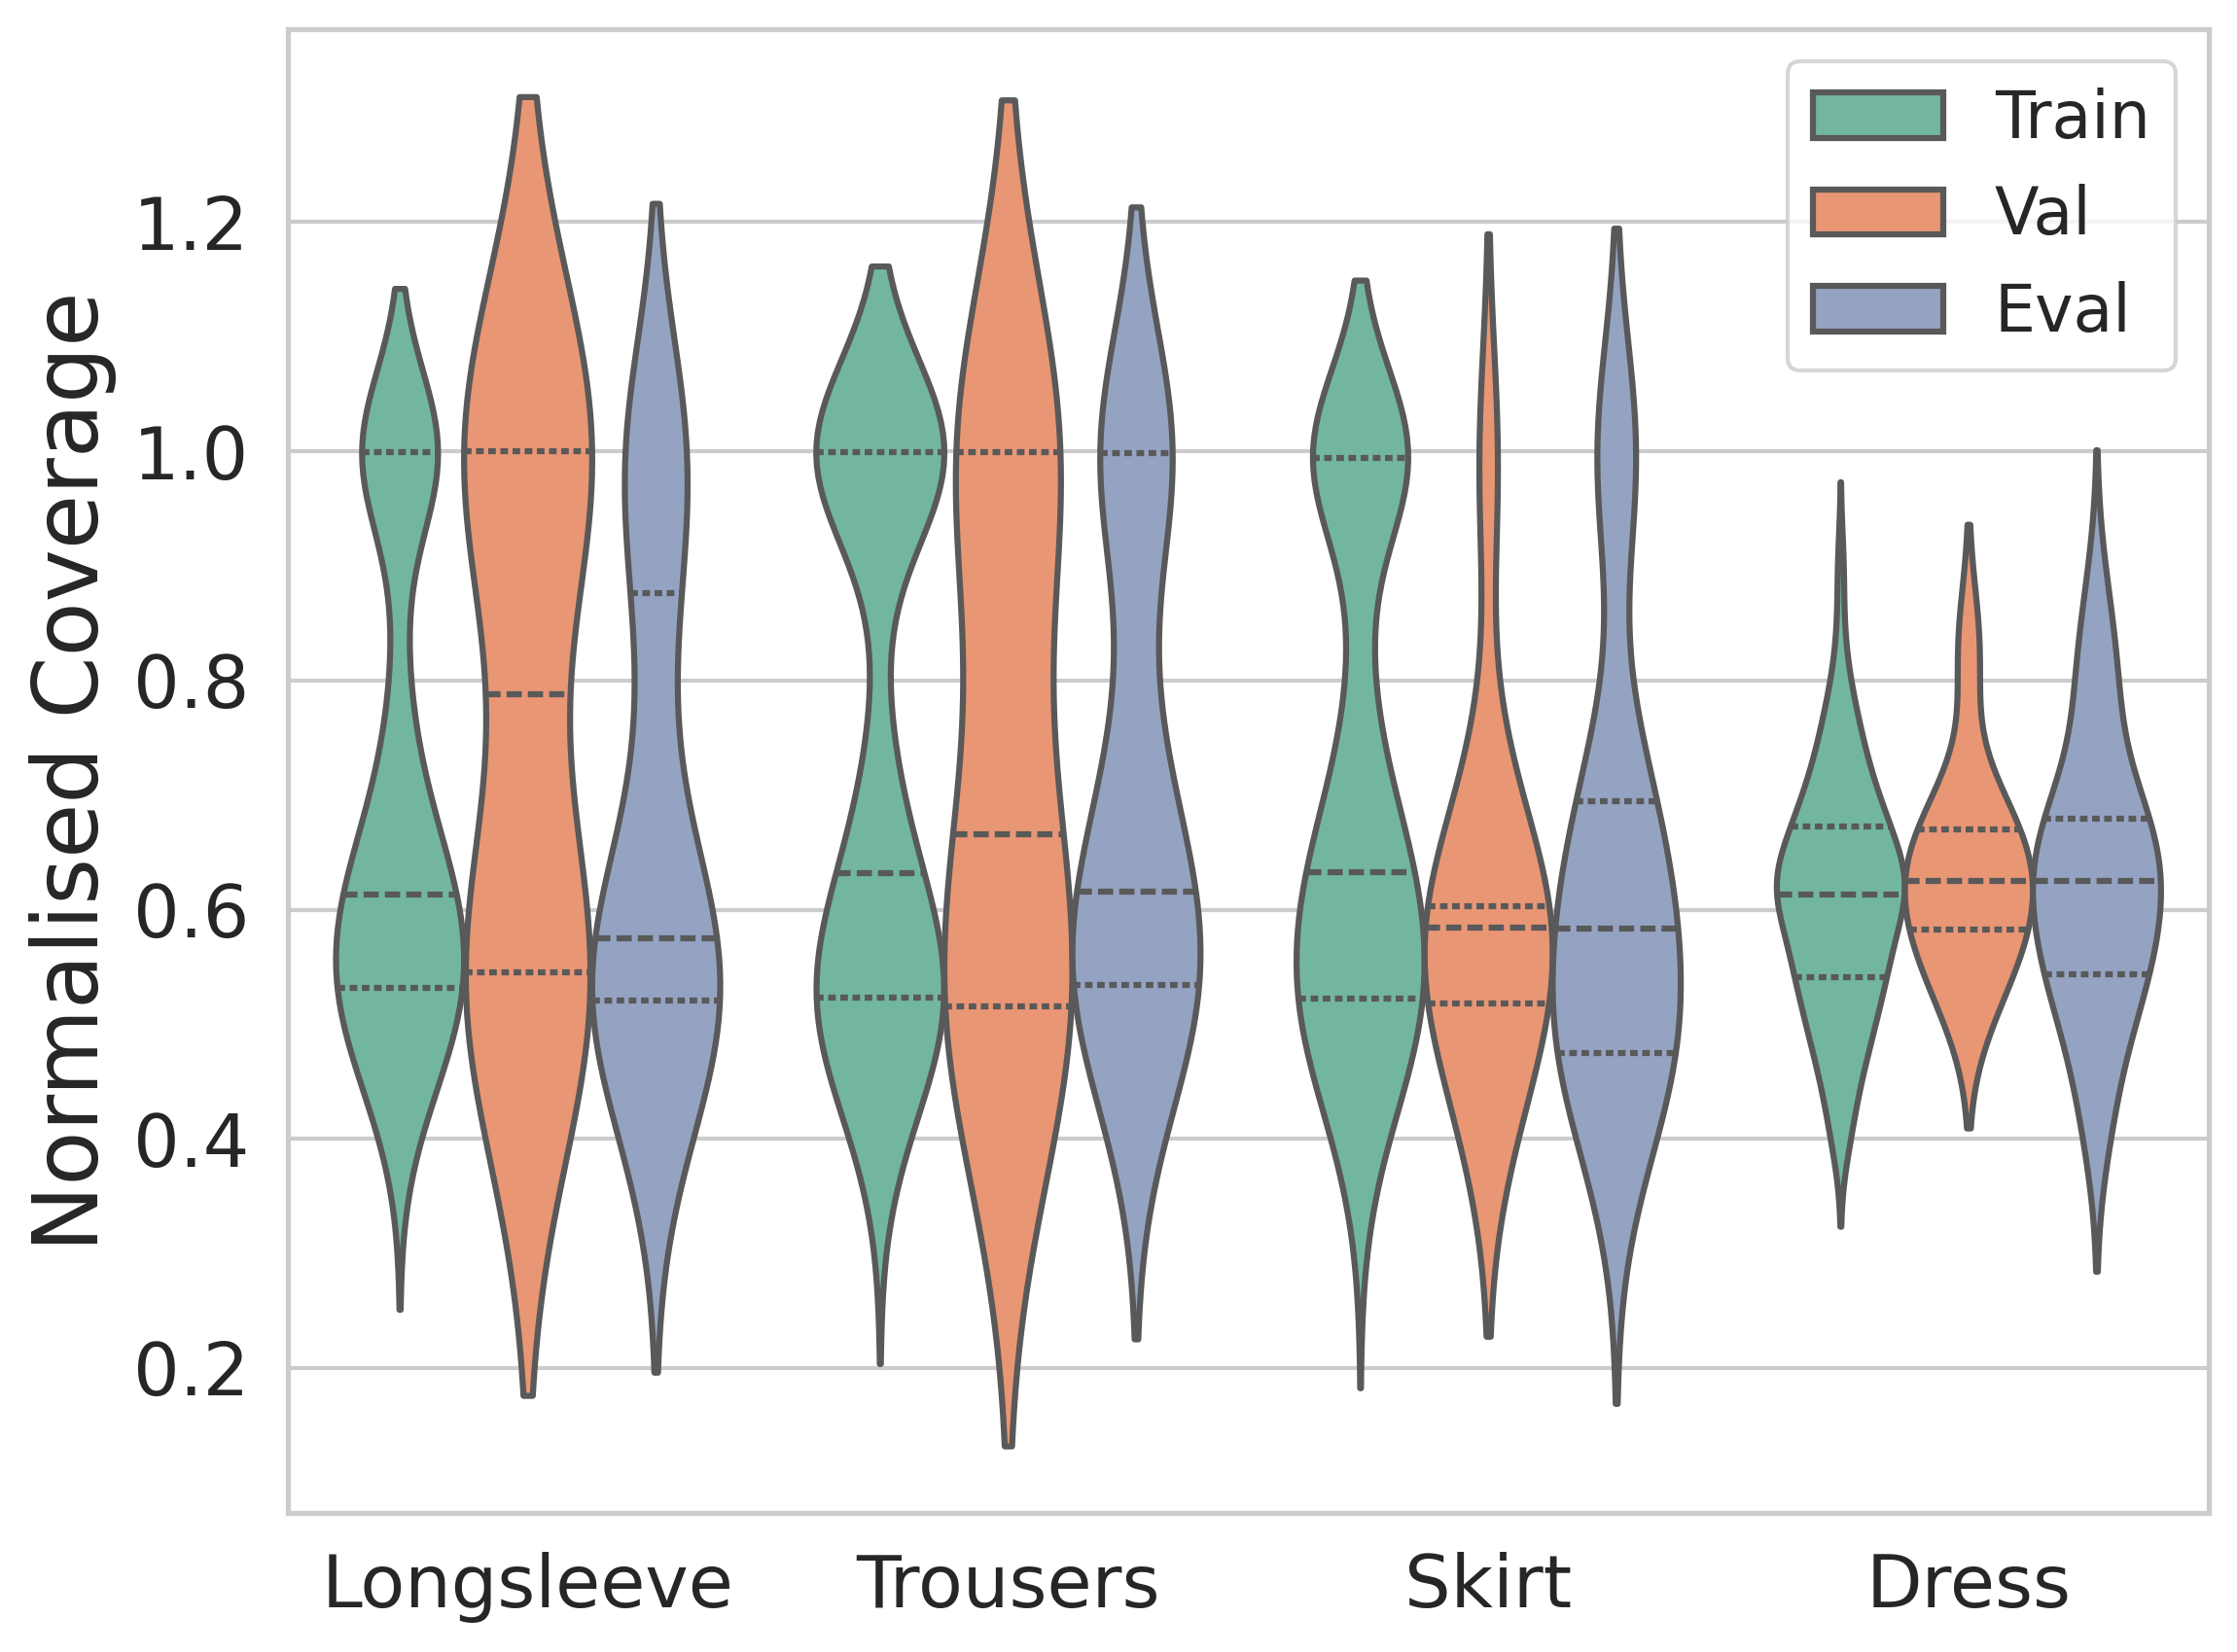
\includegraphics[width=\linewidth]{plots/normalized_coverage_distribution.png}
        \caption{Normalised Coverage Distribution}
        \label{fig:nc-dist}
    \end{subfigure}
    \begin{subfigure}[t]{0.37\linewidth}
        \vspace{0pt}
        \centering 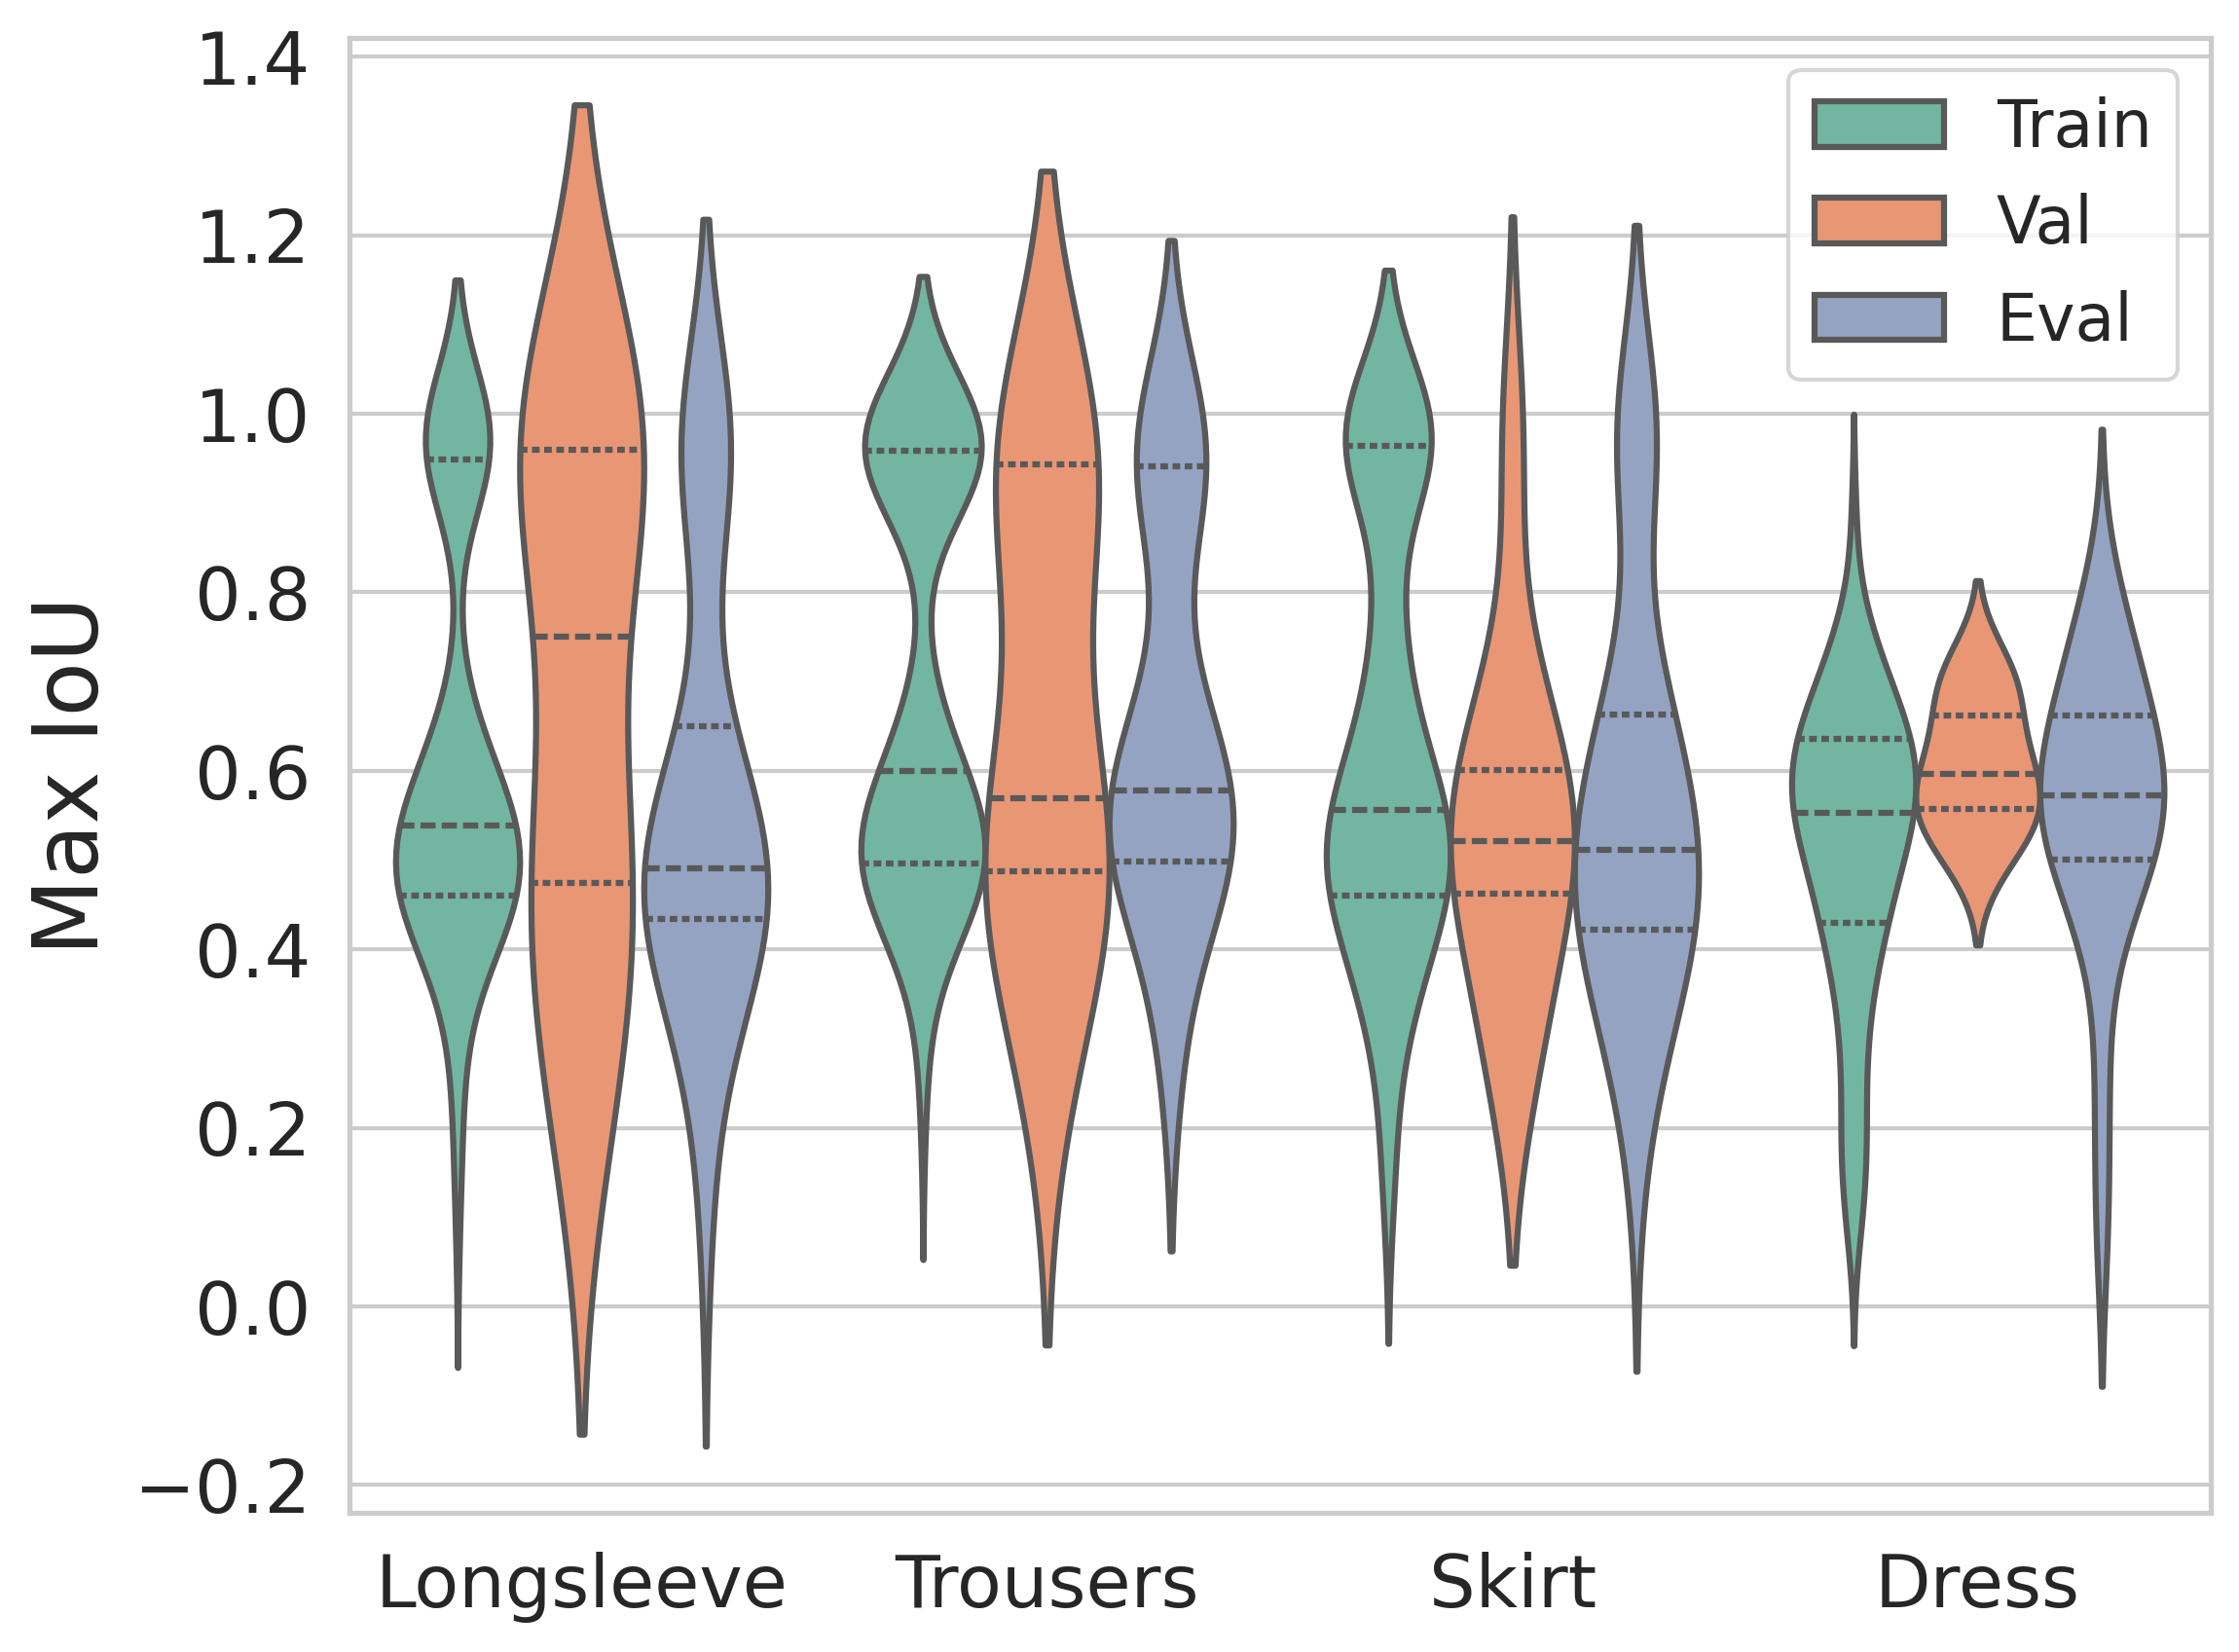
\includegraphics[width=\linewidth]{plots/max_iou_distribution.png}
        \caption{Max IoU Distribution}
        \label{fig:iou-dist}
    \end{subfigure}
    \begin{subfigure}[t]{0.24\linewidth}
        \vspace{0pt}
        \centering 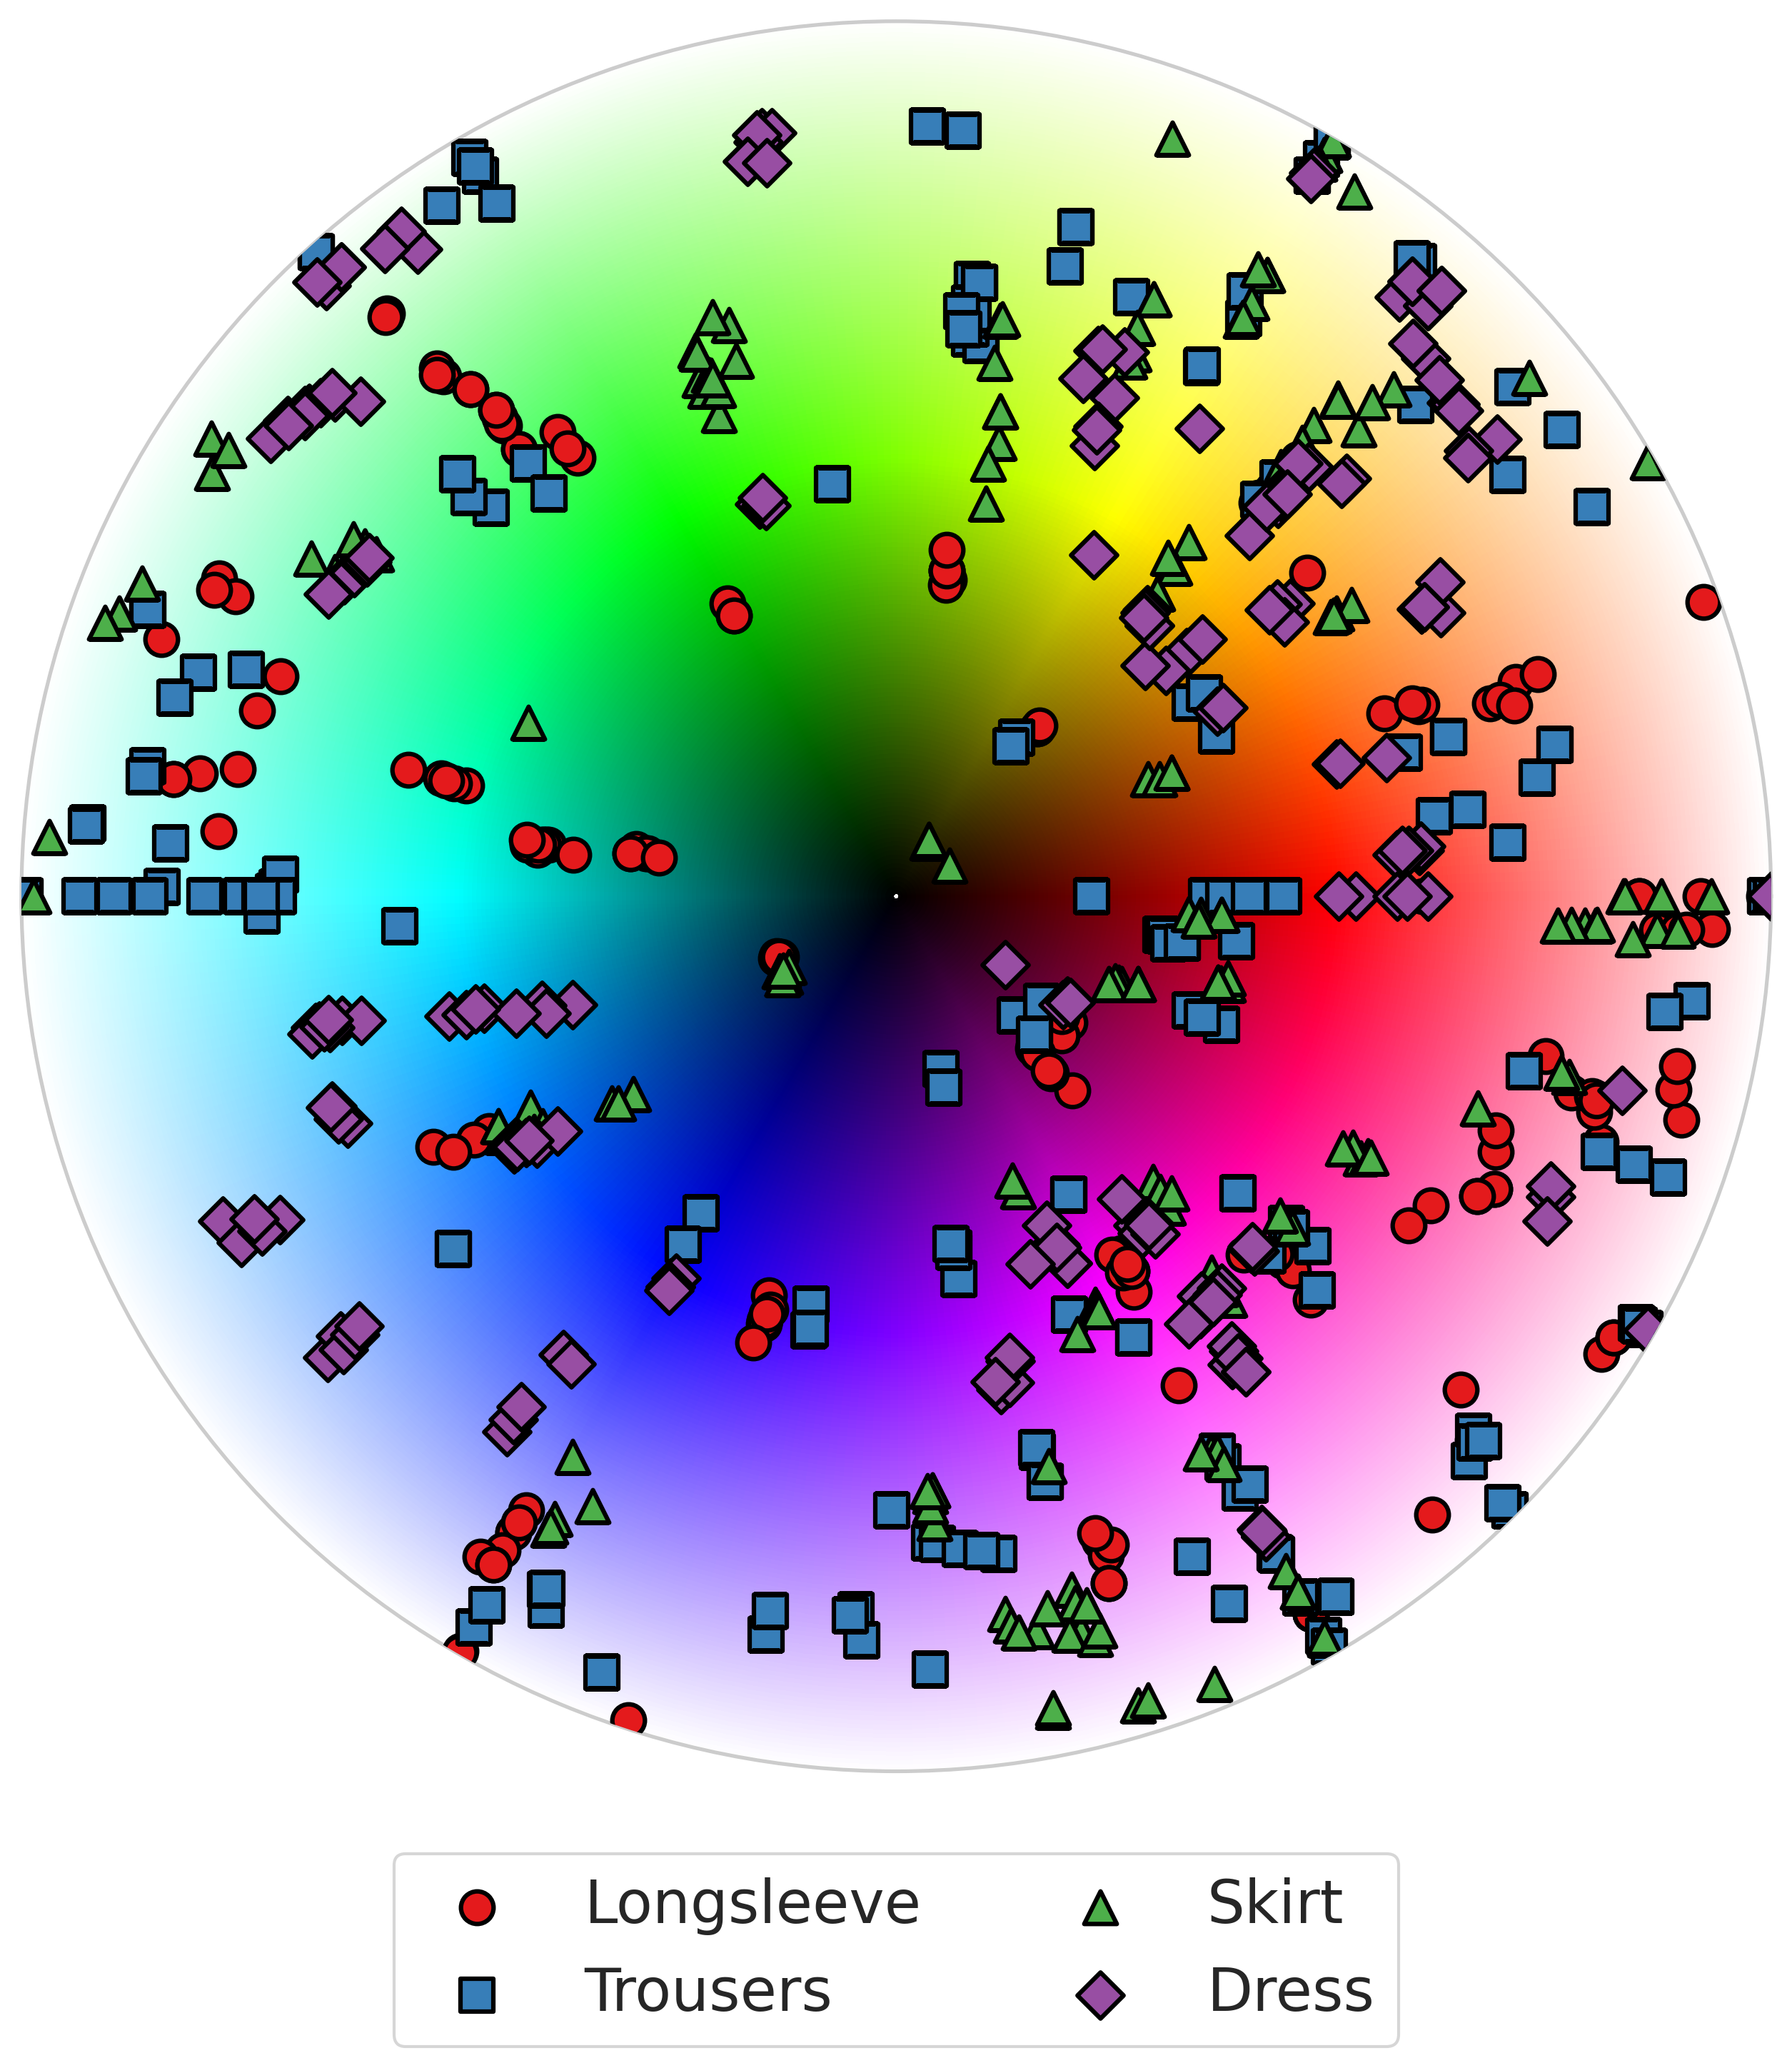
\includegraphics[width=\linewidth]{plots/colour_distribution.png}
        \caption{Colour Distribution}
        \label{fig:colour-distribution}
    \end{subfigure}
    \caption{The initial state distribution of the simulated garments.}
    \label{fig:garment-distribution}
\end{figure*}

\section{Real Robot Setup} \label{sec:real-world-setup}

In the cloth manipulation literature, robot arms are often fixed on a table \cite{lin2022learning,lee2024learning,canberk2023cloth}, leading to a ring-shaped workspace for Pick-and-Place (PnP) primitives. Real garments are generally larger than simple fabrics, so it becomes physically impossible to flatten them within a fixed square window inside the workspace of a single robot arm---a common practice in this domain \cite{kadi2025draper, hoque2022visuospatial, lee2021learning}. This requires us to develop a transfer strategy to bridge the gap between observation and the workspace in addition to the gap between the simulation and the real robot environment.
\begin{figure*}[t!]
    \centering
    
    % --- Subpart (a): Real Robot Setup ---
    \begin{subfigure}[b]{0.3\linewidth}
        \centering
        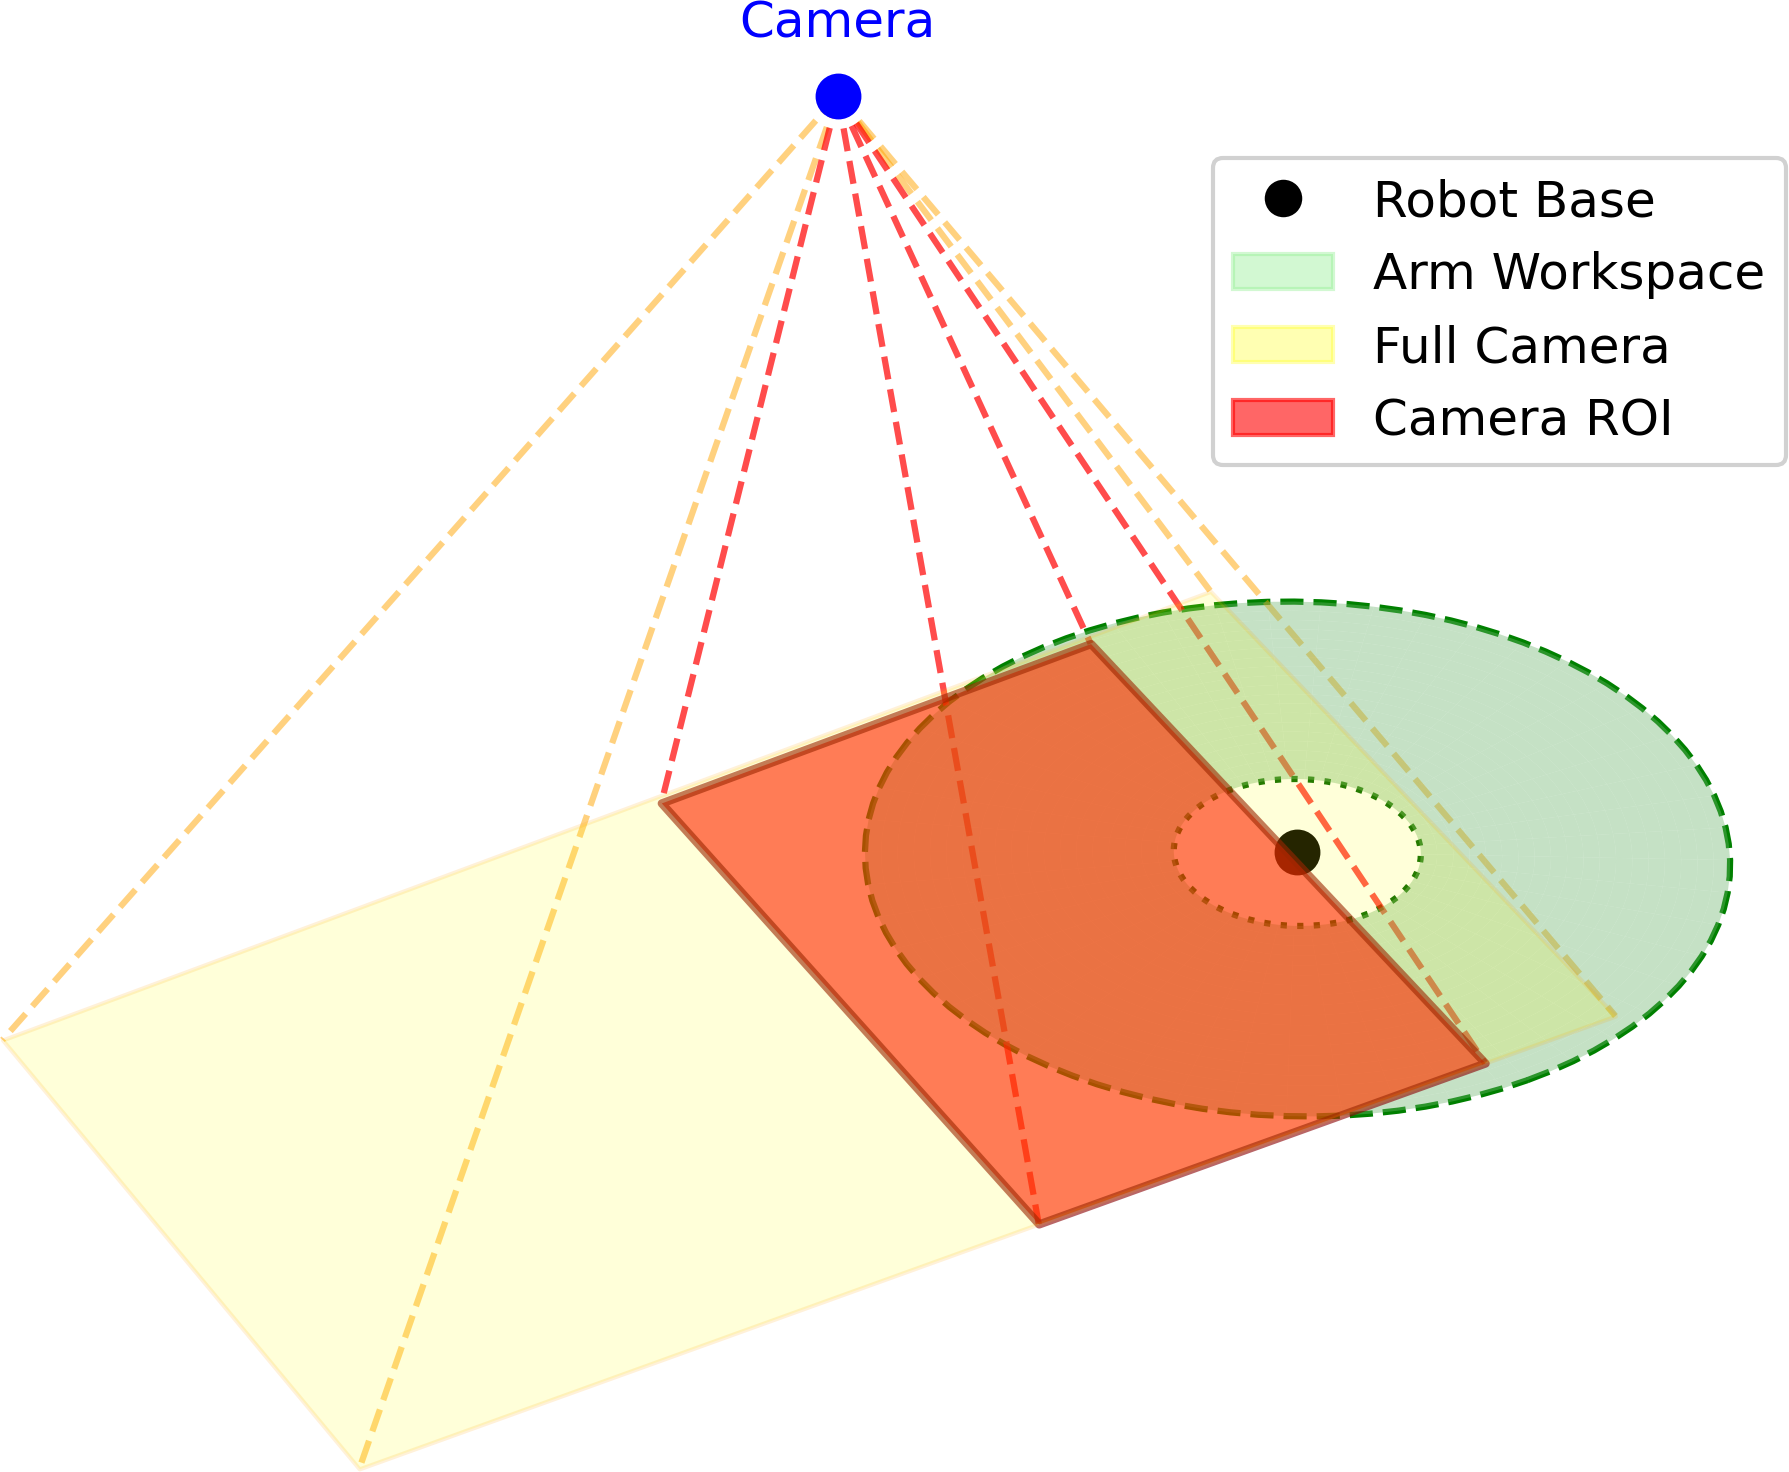
\includegraphics[width=\linewidth]{plots/tightest_cropped_plot.png}
        \caption{Camera Setup}
        \label{fig:robot-camera}
    \end{subfigure}\hfill
    % --- Subpart (b): Transfer Heuristic ---
    \begin{subfigure}[b]{0.45\linewidth}
        \centering
        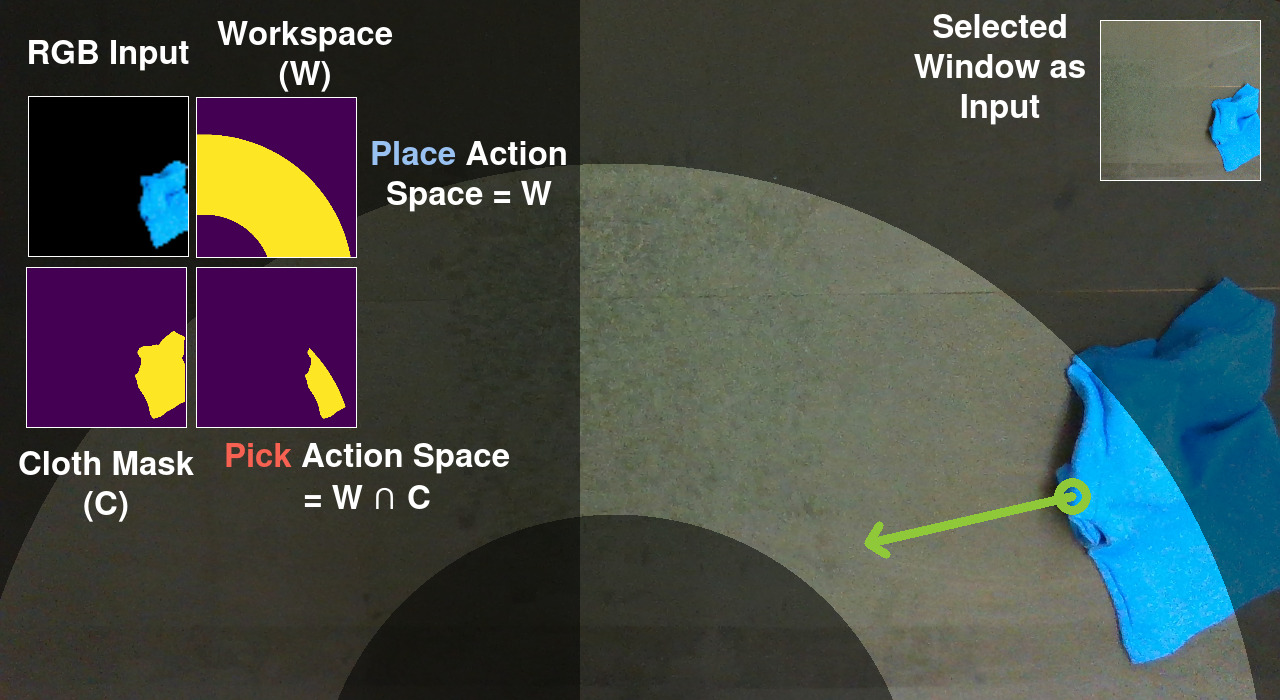
\includegraphics[width=\linewidth]{plots/transfer-hueristic-single.jpg}
        \caption{Heuristic for Transferring the Policy within the Region-of-Interest (ROI)}
        \label{fig:transfer-hueristic}
    \end{subfigure}
    % --- Subpart (c): Segmentation Parameters Table ---
    \begin{subfigure}[b]{0.24\linewidth}
        \centering
        
        \label{fig:setup_c}
        \vspace{0.5em} % Small buffer between caption and table
        \resizebox{\textwidth}{!}{
        \begin{tabular}{lc}
        \toprule
        \textbf{Camera} & \textbf{Value} \\
        \midrule
        $FoV$ & 69$^\circ$ $\times$ 42$^\circ$\\
        Camera Resolution & 1280 $\times$ 720 px\\
        RoI Resolution & 450 $\times$ 710 px\\
        RoI Start & (700, 10) px \\
        $P_c$ & (0.03, -0.86, 1.66)m \\
        $r_n, r_f$ & 0.2\,m, 0.7\,m\\
        \midrule
        \textbf{Segmentation} & \textbf{Value} \\
        \midrule
        model & \texttt{sam\_vit\_h\_4b8939} \\
        $A_{\text{min}}$  & $1,000$ \\
        $A_{\text{max}}$  & $90,000$ \\
        $\alpha_{border}$ & $0.15$\\
        $S_{\text{min}}$  & $10$ \\
        $V_{\text{min}}$ & $10$ \\
        \bottomrule
        \end{tabular}}
        \caption{Parameters \label{tab:seg-para}}
    \end{subfigure}
    
    % --- Main Overarching Caption ---
    \caption{Overview of the real-world deployment setup. (a) Camera $P_c$ is set at the front of the robot and top of the table surface; whilst the camera can capture the table view highlighted in yellow, our system operates on the Region-of-Interest (ROI) highlighted in red. (b) The heuristic approach for transferring the simulated policy to the real world; the heuristic prioritises the selection of the middle window for network inputs, but if the selected window does not contain any part of the cloth, it re-selects a window that centres around the cloth as shown; the most highlighted part of the rectangular images is the workspace of the \text{UR5e} robot for a particular action step. (c) The empirical parameters utilised in the segmentation pipeline.}
    \label{fig:real-world-overview}
\end{figure*}
As shown in Figure \ref{fig:ur5e-onrobot}, we employ a UR5e robot arm equipped with an OnRobot RG2 electric parallel gripper to conduct our real-world experiments. We position a RealSense D435i camera $P_c$ in front of the robot and above a table covered with a dark foam surface. As in simulation, we use only RGB frames with automatic exposure as input to our method in the real-world setup.

The workspace of our UR5e robot is defined by a far radius $r_{f}$ and a near radius $r_{n}$. To isolate the effective workspace, we crop the visual input to a Region of Interest (ROI) as in Figure \ref{fig:robot-camera}. Given the top-down camera perspective, we compute the spatial position $p_w$ in the world frame for each pixel $p_x$ in the camera view using the camera intrinsics and the transformation matrix. Consequently, we determine whether $p_x$ lies within the workspace by checking if $r_n \leq ||p_w - b_w||_2 \leq r_f$, where $b_w$ represents the position of the robot base in the world frame. Please refer to Table \ref{tab:seg-para} for the exact parameters of our real-robot setup. We use the UR-RTDE package \cite{urrtde2025} for conducting Cartesian planning to execute pick-and-place primitives, as it reliably produces stable trajectories.

This section first introduces the transfer heuristic, which integrates the real robot arm's workspace into LaGarNet's planning method (Section \ref{sec:transfer-hueristic}). Next, we discuss how we conduct our hand-eye calibration (Section \ref{sec:calibration}) for the transformation between the camera pixel space and robot base space. Then, we explain our approach to segmenting the physical garments from the camera observations (Section \ref{sec:real-world-cloth-seg}). Finally, we detail our grasping implementation, designed to ensure the precise and robust picking of garments (Section \ref{sec:grasping}).

\subsection{Transfer Heuristic for Robot's Ring-Shaped Workspace} \label{sec:transfer-hueristic}
Many robot manipulators face workspace constraints, such as limited reach as well as undesirable trajectories caused by inverse kinematics and joint discontinuities. These factors often make parts of the workspace unusable for smooth pick-and-place (PnP) execution. To address this general class of problems, we propose a heuristic workspace sampling method that adapts trained policies to feasible regions of a robot’s workspace without retraining. We demonstrate this method on a UR5e robot arm, whose PnP workspace resembles a ring due to both reach limitations and unstable trajectories near the base; the ring-like workspace is defined by a far radius $r_f$ and a near radius $r_n$ on the table surface.

% The \text{LaGarNet} algorithm proposed in the previous section cannot be employed directly in our real-robot setup, as the feasible square window for the pick-and-place (PnP) primitive is at most 28 cm $\times$ 28 cm for a \text{UR3e} robot arm, which is too small to flatten real garments. However, it is possible to utilise the entire ring-like workspace of the robot arm. 

% The workspace of a robot arm is often limited by its reach and the requirement to generate smooth PnP trajectories. In addition to the arm's maximum reach, we find that the workspace is also restricted by a smaller radius, within which motion planning algorithms produce trajectories that cause significant jumps in the robot arm's joint states when reaching its base. Hence, the PnP workspace of a robot arm resembles a ring

Our heuristic workspace sampling method (see Figure \ref{fig:transfer-hueristic}) builds an observation bridge between the UR5e environment and the policy's training environment. This method prioritises the central square window of the raw RGB input. If the central window does not contain any part of the cloth, it re-selects a window centred on the target cloth. The \text{LaGarNet} latent dynamics network receives observations filtered by the cloth mask in the selected window, and the model predictive control planner samples pick actions at the intersection of the cloth mask and workspace mask, and place actions within the workspace mask in the selected window. Using these two processes, we ensure that \text{LaGarNet} can be transferred to the entire visible workspace of a UR5e robot from a top-down camera for flattening real garments. Note that the dynamic cropping mechanism of the transfer heuristic is only activated at the beginning of an episode if the garment is absent from the central field of view.


\subsection{Hand-Eye Calibration} \label{sec:calibration}

To guarantee precise physical manipulation based on visual input, we conducted a rigorous eye-to-hand calibration to map the Intel RealSense camera's pixel space to the Universal Robots (UR) base frame. Our calibration target is a $5 \times 7$ ChArUco board \cite{garrido2014automatic} featuring 40~mm squares and 30.0~mm ArUco markers (Dictionary 4x4\_50) grasped by the robot's end-effector. To ensure an optimal and mathematically robust solution, we program the robot to traverse a trajectory of 50 carefully designed joint configurations. These poses explicitly sample the $SE(3)$ workspace, incorporating isolated Z-axis depth variations, lateral translations, and decoupled pitch, yaw, and roll rotations. This diverse pose generation prevents singularities and ensures the focal parameters are well-constrained. For each spatial sample, we estimate the target-to-camera transformation utilising a Perspective-n-Point solver based on the interpolated ChArUco corners. Finally, we compute the fixed camera-to-base transformation matrix by solving the standard $AX=XB$ formulation using the Park and Martin method \cite{park1994robot}.




\subsection{Real-World Garment Segmentation} \label{sec:real-world-cloth-seg}
Following standard practices in the domain \cite{canberk2023cloth, lin2022learning, kadi2025draper}, we utilise the Segment Anything Model (SAM) \cite{kirillov2023segment} to isolate the target garment. This segmentation is crucial for stripping the background from policy inputs and enabling accurate real-world evaluation. Given an RGB observation, SAM generates a set of $K$ binary candidate masks. To efficiently isolate the true garment, we convert the image to the HSV colour space and apply a multi-stage heuristic filtering pipeline. First, we apply spatial pruning: masks are retained only if their total pixel area $A \in [A_{\text{min}}, A_{\text{max}}]$. To eliminate broad background surfaces, we reject any candidate whose active border pixels exceed 30\% of the image perimeter, formalised as $P_{\text{mask}} > \alpha_{border} \times 2(h + w)$. Next, we apply chromatic and variance filters to distinguish the garment from its environment. For each mask, we compute the mean saturation $\bar{S}$ and RGB intensity variance $V$. We discard low-saturation grey areas, for which $\bar{S} < S_{\text{min}}$. We further reject grey backgrounds by ensuring $ V \geq V_{min}$. Finally, the optimal mask is selected by maximising a utility score that prioritises large, distinctly coloured objects $\text{Score}_i = A_i \cdot \bar{V}_i$. This pipeline reliably yields high-fidelity garment segmentations for downstream manipulation tasks. The specific parameters used in our real-world experiments are detailed in Table \ref{tab:seg-para}.
\subsection{Grasping} \label{sec:grasping}

Accurately grasping garments without failure remains a significant challenge for parallel grippers. We build upon the grasping protocol proposed by DRAPER \cite{kadi2025draper}, which adjusts the pick position on an eroded mask of the garment and ensures the axis connecting the two gripper fingers is perpendicular to the target mask cutline. However, while DRAPER utilises a custom pincher extension, our approach employs a standard OnRobot RG2 parallel gripper. To mitigate misgrasping errors, we initialise the gripper to a 3~cm opening width before the approach towards garments. The end-effector then executes a guarded descent, lowering gradually until the robot's force-torque sensor detects an upward reaction force of approximately 5~N. This force-based threshold ensures the garment is firmly contacted while preventing gripper faults or misgrasps caused by excessive collision resistance from the underlying workspace table.



\end{document}
